\documentclass[times, utf8, diplomski, english]{fer}
\usepackage{booktabs}
\usepackage{algpseudocode}
%\usepackage{algorithm}
\usepackage[ruled,linesnumbered]{algorithm2e}
\usepackage{subcaption}
\usepackage[mode=buildnew]{standalone}% requires -shell-escape
\usepackage{pgfplots}
\pgfplotsset{compat=newest}
\usepackage{tikz}
\usetikzlibrary{arrows,automata}
\usetikzlibrary{positioning}
\usetikzlibrary{calc}
\usetikzlibrary{patterns}
\usetikzlibrary{backgrounds}
\graphicspath{{./slike/}}
\usepackage{floatrow}
\usepackage{hyperref}
\newfloatcommand{capbtabbox}{table}[][\FBwidth]%\algtext*{EndFor}% Remove "end fot" text
\begin{document}

% TODO: Navedite broj rada.
\thesisnumber{1527}

% TODO: Navedite naslov rada.
\title{From Global to Local: Maintaining Accurate Mobile Manipulator State Estimates Over Long Trajectories}

% TODO: Navedite svoje ime i prezime.
\author{Filip Maric}

\maketitle

% Ispis stranice s napomenom o umetanju izvornika rada. Uklonite naredbu \izvornik ako želite izbaciti tu stranicu.
\izvornik

% Dodavanje zahvale ili prazne stranice. Ako ne želite dodati zahvalu, naredbu ostavite radi prazne stranice.
\zahvala{dsadsa}

\tableofcontents

\chapter{Introduction}
In applications ranging from military operations to extraterrestrial exploration, mobile manipulators present themselves as the ideal answer to many challenges being addressed by robots.
The mobile platform increases the workspace of a conventional manipulator while also enabling optimal positioning.
The increased workspace also provides the capability of performing industrial tasks that would otherwise require multiple manipulators.
A comprehensive survey on mobile manipulator systems can be found in \citep{bloch2003nonholonomic}.

The mobile manipulator can be described as a robotic system composed of a manipulator arm mounted on top of a mobile platform.
A variety of issues related to mobile manipulators have been explored in the past two decades. 
These include dynamic and static stability, force development and application, maximum payload determination, etc. \citep{papadopoulos1999framework,korayem2004analysis}.
However, a majority of the research concerning mobile manipulators deals with motion planning and state estimation \citep{yamamoto1992coordinating,korayem2012mathematical}.
 
This thesis explores the problems of state estimation and motion planning in the context of an omni-directional mobile manipulator.
Chapter \ref{chapter:thing} introduces the "Thing" mobile manipulator used in this work.
Each major component is described in appropriate detail, keeping in mind the context of research presented.

Chapter \ref{chapter:State estimation} deals with the challenge of state estimation for a mobile manipulator.
Assuming accurate mobile base pose data, it is possible to estimate the state of the manipulator to a reasonable degree of accuracy using only a forward kinematics model described in section \autoref{section:Kinematics}.
The primary interest thus lies in obtaining the end effector pose estimate, as other estimates can be derived from it if necessary.
Finding the base position relative to the starting position is explored in section \autoref{section:Localization} by fusing local odometry estimates in a probabilistic framework.

Finally, two approaches two motion planning are described in chapter \autoref{chapter:motion planning}.
A classical approach enables defining priorities for kinematics tasks assigned to the robot, which are then applied in a classical optimization scheme.
The more contemporary \textit{sequential convex optimization} is also explored, which enables defining non-linear inequality and equality constraints. 
These two approaches offer a powerful framework for local motion planning and trajectory optimization.


\chapter{Thing mobile manipulator}\label{chapter:thing}
The Thing mobile manipulator (\autoref{figure:thing}) is composed of a Ridgeback omni-directional platform and a UR10 manipulator arm with a Robotiq 3-Finger Adaptive Robot Gripper in place of the end-effector.
The three systems are essentially separate on the lower level: the Ridgeback, UR10 and Robotiq gripper local hardware interfaces are electronically independent self-contained systems.
These local interfaces are unified by the Ridgeback's computer, which operates as a server under the Robot Operating System (ROS).
This interfacing strategy provides all the advantages of distributed computing, such as networked control or information sharing.
\begin{figure}[h]
\centering
\includegraphics[scale=0.045]{thing_segmented_trans}
\caption{The Thing mobile manipulator}
\label{figure:thing}
\end{figure}
This platform is also equipped with a vast array of sensors, making it ideal for autonomous robotics research.
The Ridgeback platform is outfitted with a Hokuyo laser range finder (LIDAR) and Kinect2 camera , extending both planar and spatial perception capabilities.
The omni-directional drive enables field-of-view (FOV) control independent of both end-effector pose and base position, making it an interesting platform for active perception research.
The UR10 manipulator is equipped with the FT300 force-torque sensor and an Intel Realsense camera mounted on the gripper, further increasing perception capabilities.
\section{Ridgeback} 
The Ridgeback (\autoref{fig:ridgeback}) is a midsize indoor robot platform that uses an omni-drive to move manipulators and heavy payloads with minimal constraints. 
The omnidirectional base provides precision positioning in constrained environments and comes fully integrated with on-board computer, front laser range finder and an IMU. 
Ridgeback offers native ROS and Gazebo integration and is compatible with a wide range of robot accessories.
\begin{figure*}[h]
    \centering
        \begin{subfigure}[t]{0.34\textwidth}
        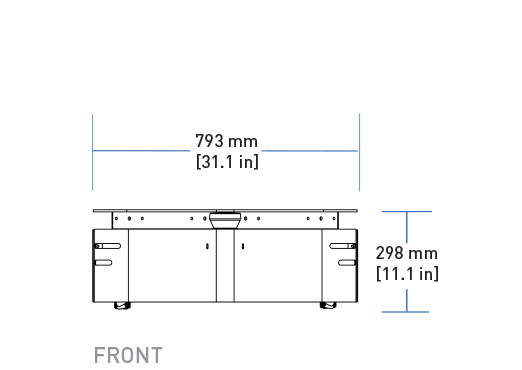
\includegraphics[width=\textwidth]{rb_front}
        \caption{Front}
        %\label{fig:gull}
    \end{subfigure}
    ~
    \begin{subfigure}[t]{0.34\textwidth}
        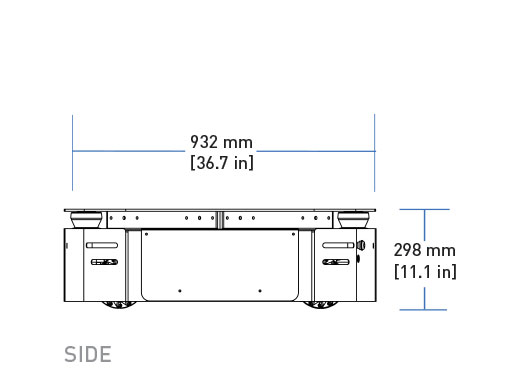
\includegraphics[width=\textwidth]{rb_side}
        \caption{Side}
        %\label{fig:gull}
    \end{subfigure}
     %add desired spacing between images, e. g. ~, \quad, \qquad, \hfill etc. 
      %(or a blank line to force the subfigure onto a new line)
    \begin{subfigure}[t]{0.34\textwidth}
        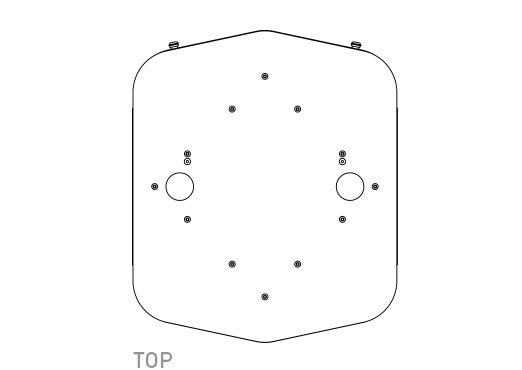
\includegraphics[width=\textwidth]{rb_top}
        \caption{Top}
        %\label{fig:tiger}
    \end{subfigure}
     ~%add desired spacing between images, e. g. ~, \quad, \qquad, \hfill etc. 
    %(or a blank line to force the subfigure onto a new line)
    \begin{subfigure}[t]{0.34\textwidth}
        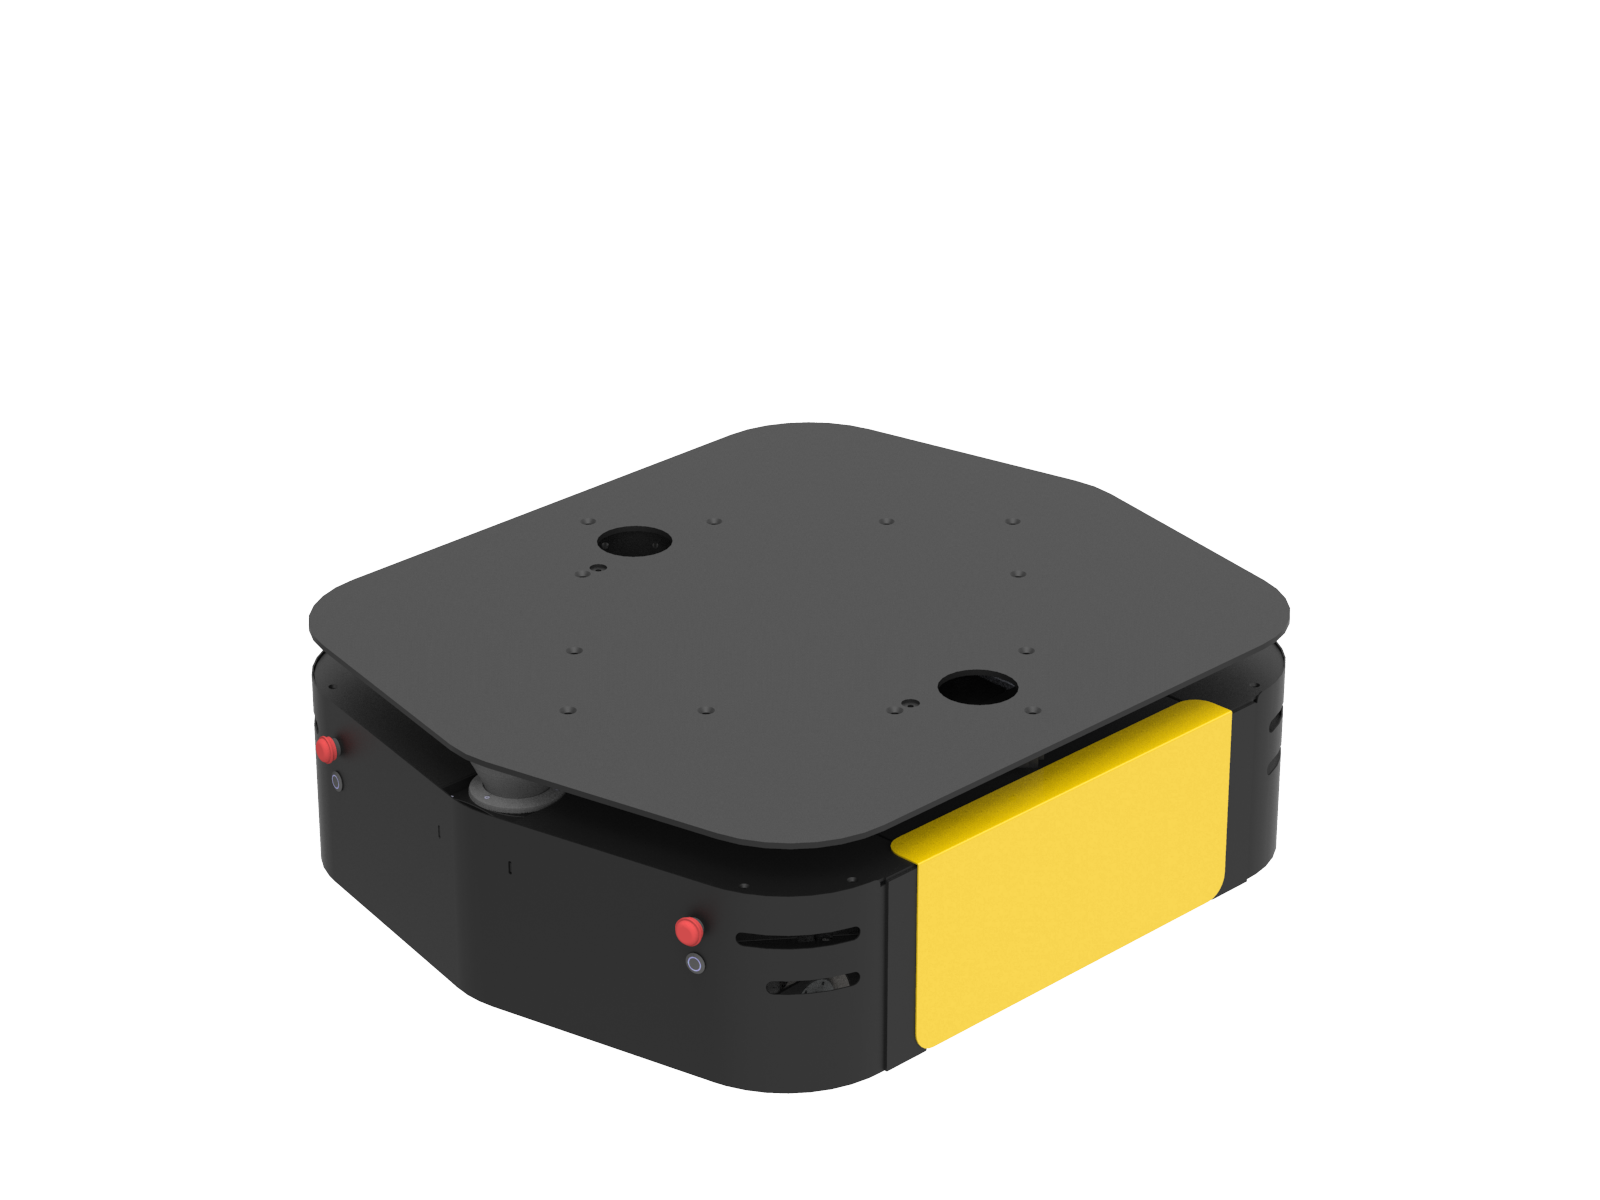
\includegraphics[width=\textwidth]{ridgeback}
        \caption{Render}
        %\label{fig:mouse}
    \end{subfigure}
    \caption{The Ridgeback mobile platform}\label{fig:ridgeback}
\end{figure*}
It is primarily designed for warehousing applications as it is highly flexible in a controlled flat environment.
The built in wheel odometry provides accurate local position estimates, with pose drift accumulating very slowly.
For improved localization and obstacle avoidance, the navigation stack ROS package provides SLAM capability using the on-board LIDAR and IMU.

In a controlled laboratory setting, this platform enables a high degree of flexibility in research.
The high load bearing capability enables the platform to carry manipulators (such as the UR10) and large sensor arrays.

\newpage
\section{UR10} 
The UR10 is Universal Robotics largest collaborative industrial manipulator.
It is a full 6DOF robotic arm capable of mimicking human arm movements.
During operation it can handle weights up to 10 kg, making it viable for a wide range of tasks.
The provided drivers enable performing collaborative tasks alongside human operators, allowing for easy positioning of the arm through compliant movement and preventing use of excessive force on impact.
\begin{figure}[h]
\begin{floatrow}
    \ffigbox{
        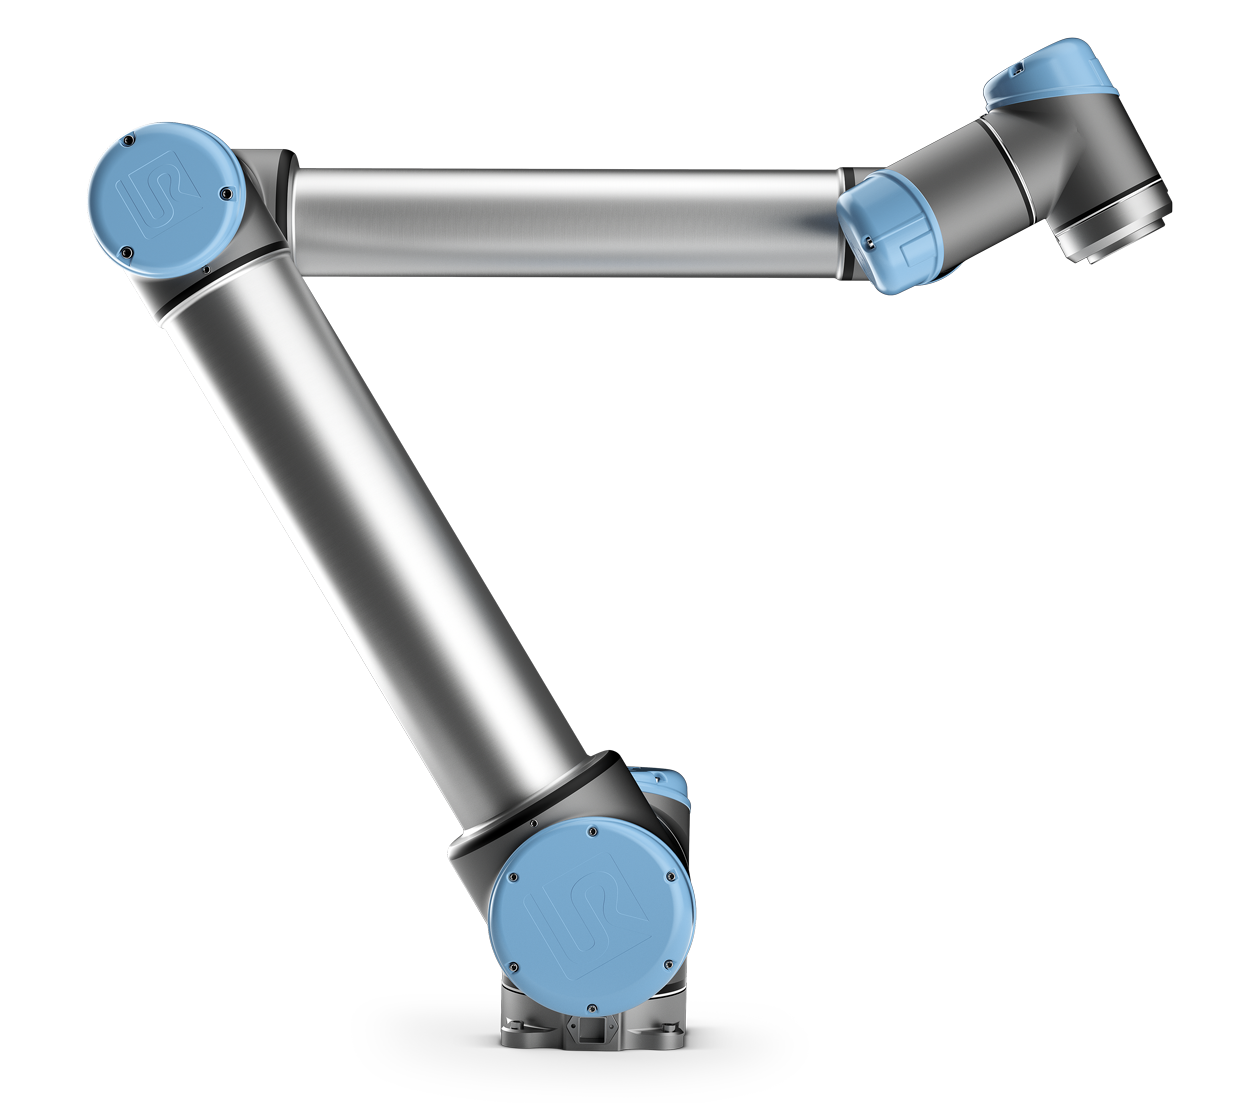
\includegraphics[width=0.34\textwidth]{ur10_right}
        }{
    \caption{The UR10 manipulator}\label{fig:ur10}
    }
    \capbtabbox{
\begin{tabular}{@{}lll@{}}
\toprule
\textbf{{ Weight}}&  28.9 kg& \\ \midrule
\textbf{{Payload}}&  10 kg&  \\ \midrule
\textbf{{Speed}}&  {\footnotesize Large joints: Max 120$^{\circ}$/s}&  \\
&  {\footnotesize Wrist joints: Max 180$^{\circ}$/s}&   \\
&  {\footnotesize Tool: approx 1 m/s}& \\ \midrule
\textbf{{\small Repeatability}}& $\pm0.01$ mm& \\ \midrule
\textbf{Power}& average 350 W& \\ \bottomrule
\end{tabular}
}{
\caption{UR10 specifications}
\label{tab:ur10 specs}
}
\end{floatrow}
\end{figure}

The data in table \autoref{tab:ur10 specs} clearly shows that the UR10 manipulator is meant for tasks involving high precision and light payloads. 
The repeatability value of $0.01$ mm shows that the UR10 can reach the same pose multiple times with a high degree of accuracy, which is important in industrial applications.
Additionally, it's light weight and high end-effector modularity make it ideal for research purposes.

\section{Hokuyo LIDAR}
The Hokuyo UST-10LX Scanning Laser Rangefinder is a small, accurate, high-speed device for obstacle detection and localization of autonomous robots and automated material handling systems. 
This model uses Ethernet interface for communication and can obtain measurement data in a wide field of view up to a distance of 10 meters with millimeter resolution.
%\begin{figure*}[t!]
%    \centering
%        \begin{subfigure}[t]{0.2\textwidth}
%        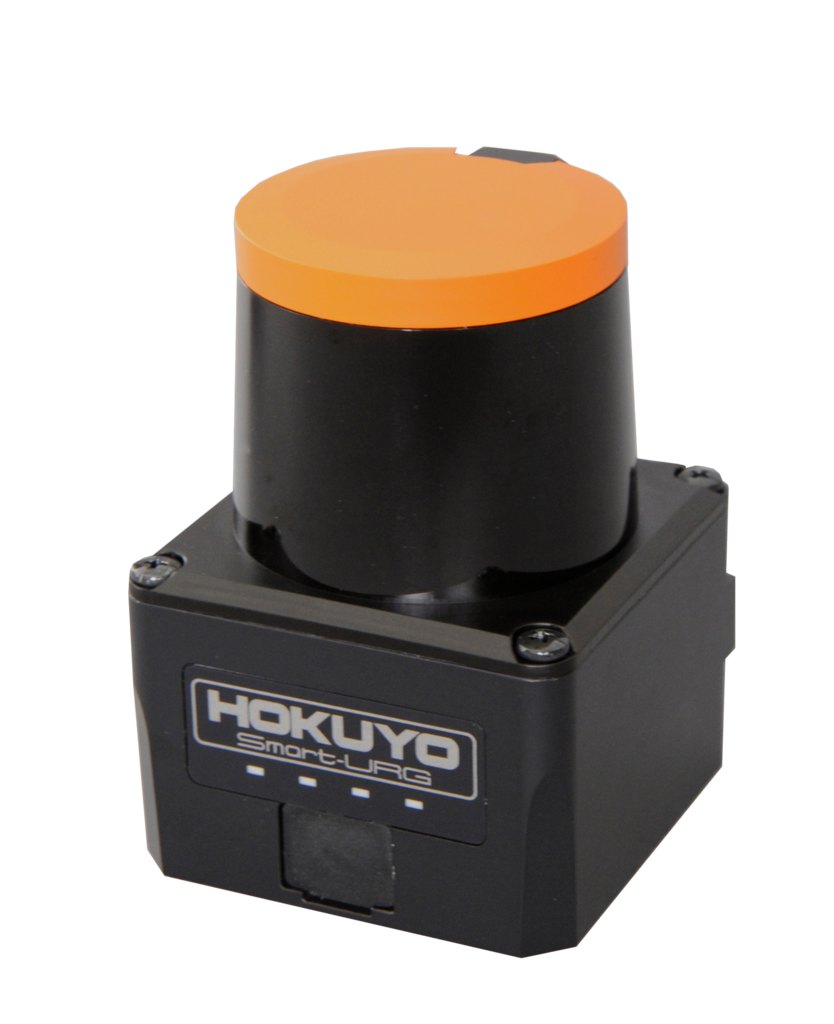
\includegraphics[width=\textwidth]{hokuyo_pic}
%    \end{subfigure}
%    \caption{The Hokuyo UST-10LX LIDAR}\label{fig:ur10}
%\end{figure*}
This sensor uses a laser source to scan 270$^\circ$ field of view. Positions of objects in the range are calculated with step angle and distance. Sensor outputs these data through communication channel.

\section{FT300}
\begin{figure*}[t!]
    \centering
        \begin{subfigure}[h,t]{0.34\textwidth}
        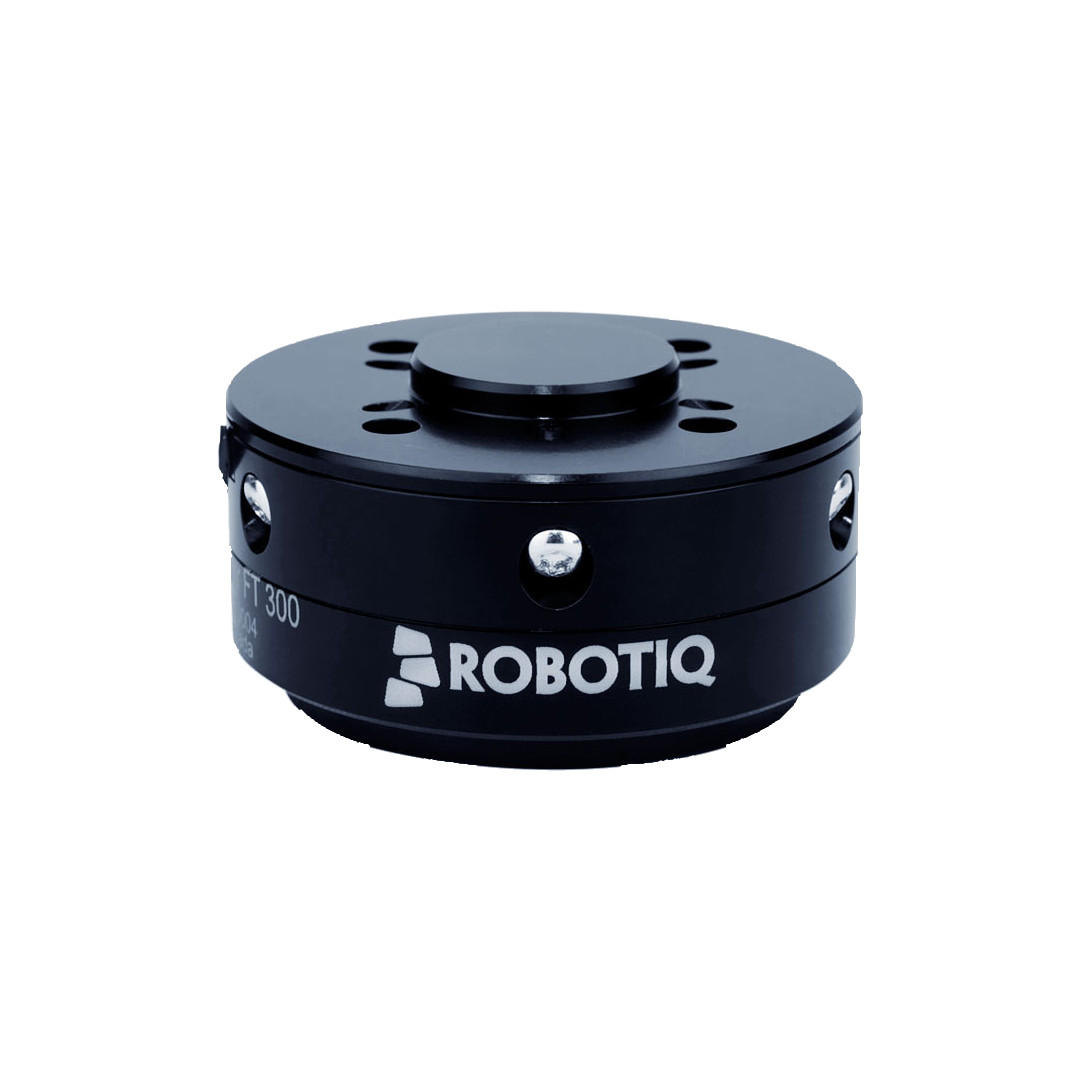
\includegraphics[clip, trim=0cm 5cm 0cm 5cm, width=\textwidth]{FT300_pic}
        \caption{Front}
        %\label{fig:gull}
    \end{subfigure}
    ~
    \begin{subfigure}[h,t]{0.34\textwidth}
        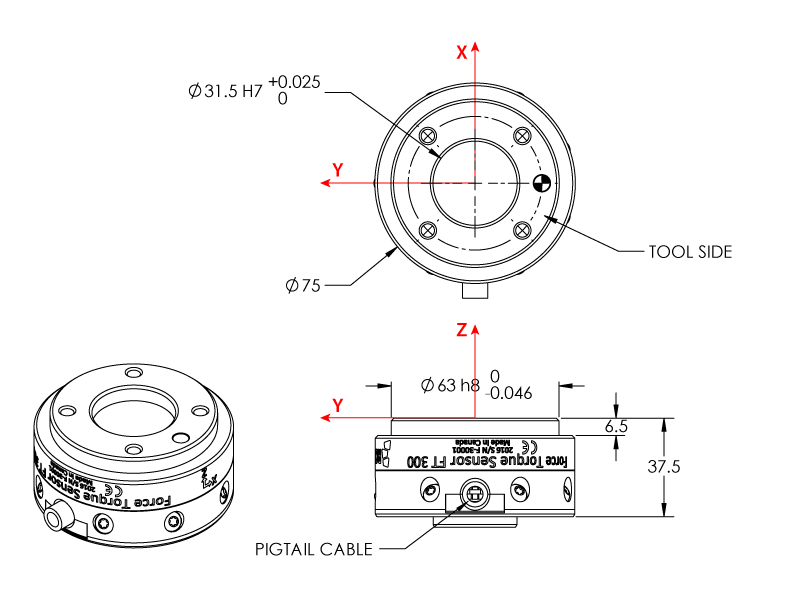
\includegraphics[width=\textwidth]{FT300}
        \caption{Side}
        %\label{fig:gull}
    \end{subfigure}
    \caption{The FT300 force-torque sensor}\label{fig:FT300}
\end{figure*}
The UR10 on the Thing mobile manipulator has a variety of sensors built-in for use in various tasks.
One such sensor is the FT300 force-torque sensor by Robotiq.
In terms of mechanical fit, the Sensor has an embedded coupling to fit directly on the UR wrist. The tool side of the Sensor matches the UR bolt pattern. 
It-s application range from impedance control to perception and contact calibration of the manipulator.


\section{Robotiq Gripper}
\begin{figure}[h]
\centering
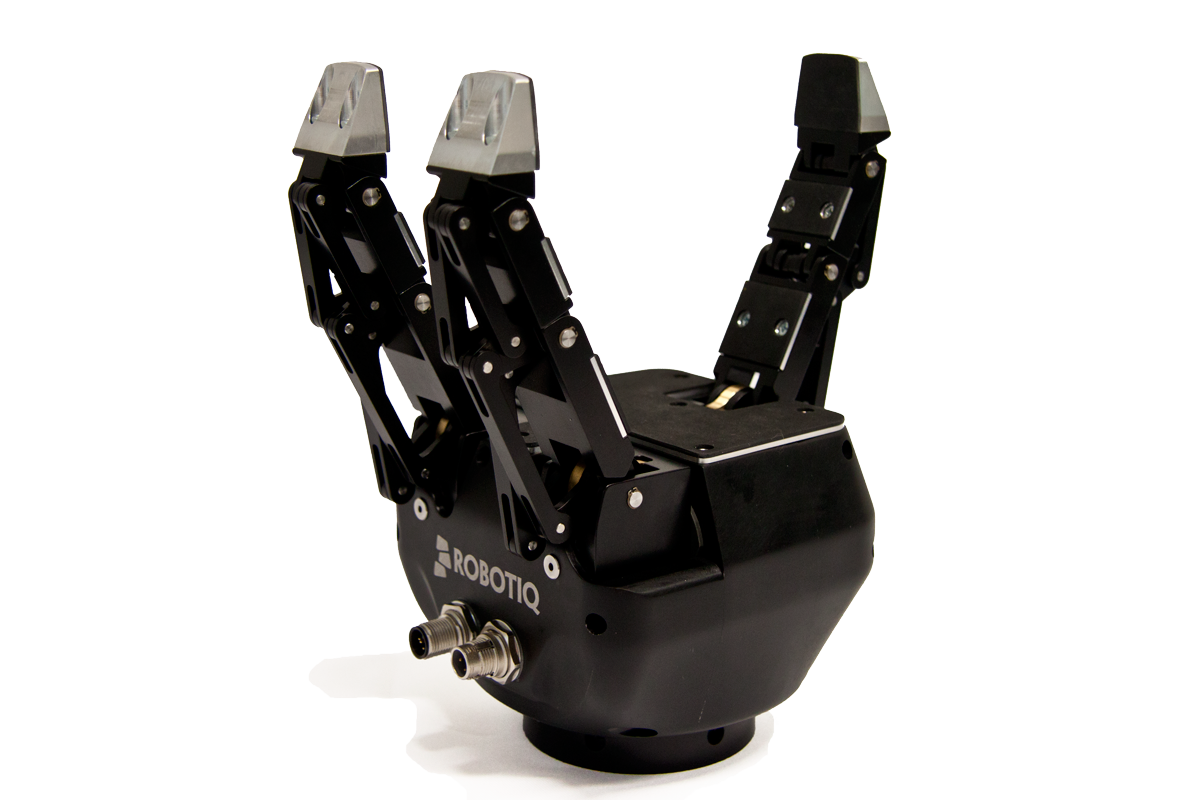
\includegraphics[width=0.3\textwidth]{robotiq}
\caption{The Robotiq gripper}
\end{figure}
The Robotiq gripper is a three-fingered adaptive gripper used as the end effector on the UR10 manipulator.
It is created for applications in advanced manufacturing and robotics research. 
All the fingers can be independently position,velocity and force controlled and can exert forces from 50 to 60 $N$ at the finger tips.




\chapter{State estimation}\label{chapter:State estimation}
State estimation is an often encountered challenge when working with autonomous systems.
Most autonomy schemes require accurate information on the current state of the system in order properly modify the system behaviour.
This type of system can be generalized as a non-linear system described by a difference equation and observation model with additive noise \footnote{we leave out separate expressions for input variables as they can be integrated within the functions $f$ and $h$}
\begin{subequations}\label{eq:state_space_nl}
\begin{gather}
x_k = f\left(x_{k-1}\right) + w_{k-1} , \ x \in \mathbb{R}^n \\
z_k = h\left(x_k\right) + v_k, \ z \in \mathbb{R}^k
\end{gather}
\end{subequations}
Finding the state estimate $\hat{x}_k$ given the measurements $z_0 \dots z_k$ subject to measurement noise $v$ and past states $x_0 \dots x_{k-1}$ subject to process noise $w$ is the state estimation problem.
Various algorithms have been developed using different mathematical frameworks to find the best estimate according to some optimality criterion (\cite{thrun2005probabilistic}).  
\begin{figure}[h]
\centering
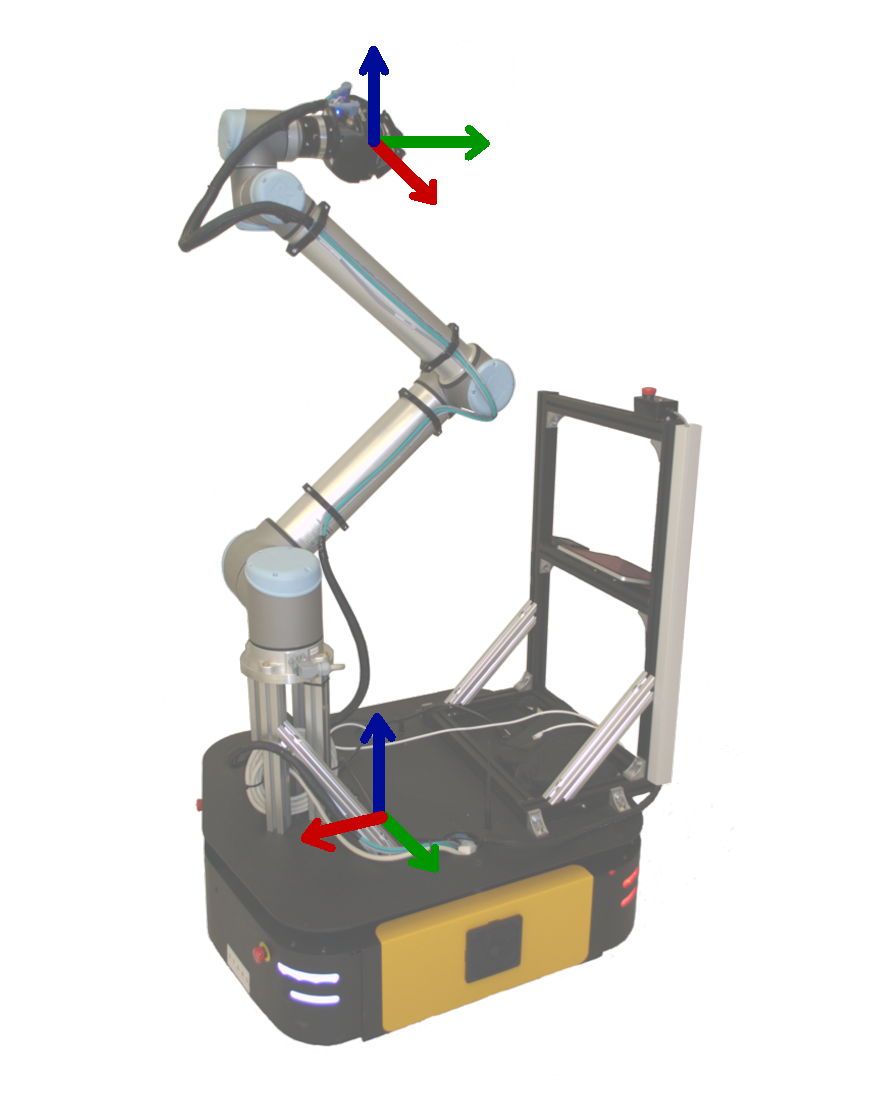
\includegraphics[scale=0.4]{Thingtr}
\caption{The Thing mobile manipulator and the frames subject to estimation}
\label{figure:thing states}
\end{figure}

The problem of state estimation for a mobile manipulator is twofold: it is necessary to estimate the state of the end-effector in the local workspace while also placing it in the global context of a map or starting position.
The local state of the end-effector is successfully estimated using a deterministic kinematic model.
Joint position values are used to provide a state estimate, ignoring various dynamic and environment effects.
Estimating the base state (\textit{localization}) is a more complex problem; the dynamic and environment effects on base movement significantly affect the steady-state.
Consequently, in addition to kinematic models we have to rely on movement estimates from sensor data which is inherently noisy.
The imperfect model and sensor data are fused in a single estimate using a probabilistic framework.

In this chapter, we first define our state of interest (as seen in \autoref{figure:thing states}) in \autoref{section:State}. 
Section \ref{section:Kinematics} contains details on the derivation of the kinematic model used in end-effector state estimation assuming sufficient knowledge of the base pose. 
The probabilistic framework used for estimating the base state is described in \autoref{section:Localization}, where wheel and LIDAR odometry are fused to provide an accurate estimate.
%The focus of this chapter is estimating the pose of the end-effector and mobile base, but the methods are extendable to any frame on the platform.

\section{State}\label{section:State}
Control and task algorithms frequently require information on the pose of the mobile manipulator frames in Cartesian space. 
A frame pose represents complete information about a frames position and orientation in a given reference frame.
The pose is often represented by a \textit{homogenous transformation matrix}
\begin{align}
T_{k-1}^k =
\begin{bmatrix}
R & p\\
0 & 1\\
\end{bmatrix}\,.
\label{eq:transform}
\end{align}
The rotation matrix $R \in \mathbb{R}^{3x3}$ represents the orientation of the frame $k$ relative to the frame $k-1 $, while translation is represented by the vector $p \in \mathbb{R}^3$.
Estimating the matrix $T$ for the end-effector is a 9-dimensional problem which can be further reduced. 
It is possible to fully define it the vector $r$ consisting of the translation vector $p$ and a \textit{quaternion} $q$
\begin{align} 
r_{EE}\left(T_{0}^{EE}\right) = 
\begin{bmatrix}
x& y& z& q_w& q_x& q_y& q_z
\end{bmatrix}^T\, .
\label{eq:pose}
\end{align}
The number of dimensions can also be reduced for the base, as it moves on a 2D plane and thus only rotates alongside one axis and has a constant $z$ coordinate
\begin{align}\label{eq:pose base}
r_{B}\left(T_{0}^{B}\right) = 
\begin{bmatrix}
\hat{x}& \hat{y}& \hat{\theta}
\end{bmatrix}^T\, .
\end{align}
The estimated state consists of end-effector and base poses comes in the form of a 10-dimensional \textit{task vector} $s$
\begin{align}\label{eq:task_vector}
s = 
\begin{bmatrix}
r_{EE}& r_B
\end{bmatrix}^T
\end{align}
Using this representation, the state estimation problem has been reduced from 24 down to 10 dimensions.
Reducing the dimensionality of the problem makes it computationally less expensive, which is vital for real-time operation.
Considering that the global state estimate in this work is derived exclusively from base odometry data, it is possible to infer the base pose knowing the end-effector pose.
However, to maintain generality the formulation in \eqref{eq:pose} and \eqref{eq:pose base} is kept.

\section{Kinematic model}\label{section:Kinematics}
Disregarding the various dynamic and environment effects, the Thing can be modelled as manipulator.
The Ridgeback platform is system with holonomic constraints and it's global position and the orientation can be viewed as a chain of two prismatic and a rotational joint. 
These three joints make up the base upon which we add the kinematic model of the UR10 manipulator.
This results in a system kinematically indistinguishable from a redundant manipulator.

The UR10 joint position measurements are reasonably accurate and thus this model can be used to produce a valid local end-effector state estimate.
Assuming valid estimates for the base position and orientation, this model will accurately represent the global state of the mobile manipulator.
\subsection{Forward kinematics}\label{subsection:FK}
Forward kinematics are defined as a set of equations that express the pose of a certain frame on a kinematic chain as a function of configuration-space values
\begin{align}\label{eq:config_matrix}
q = 
\begin{bmatrix}
q_0& q_1& q_2& q_3& q_4& q_5& \hat{x}& \hat{y}& \hat{\theta}
\end{bmatrix}^T \quad .
\end{align}
The equations are commonly derived using the transforms defined in \eqref{eq:transform}.
The transform between two frames can be defined as a function of only four parameters using the Denavit-Hartenberg notation \citep{uicker1964iterative}.
\begin{align}
T_{k-1}^k(d, \ \theta, \ a, \ \alpha)
=
\begin{bmatrix}
\cos\theta_{k}& -\cos\alpha_{k}\sin\theta_{k} & \sin\alpha_{k}\sin\theta_{k} & a_k\cos\theta_{k}\\
\sin\theta_{k}& \cos\alpha_{k}\cos\theta_{k} & -\sin\alpha_{k}\cos\theta_{k} & a_k\sin\theta_{k}\\
0 & \sin\alpha_{k} & \cos\alpha_{k} & d_{k}\\
0 & 0 & 0 & 1\\
\end{bmatrix} \quad .
\label{eq:homogenous}
\end{align}
The parameters $a, \alpha$ are usually constant and represent the structure, while $d, \theta$ represent the prismatic and rotational joint values and biases.
Using the DH parameters as defined in \autoref{DH}, we derive all the transforms \eqref{eq:homogenous} from global frame to the end effector frame.
Multiplying these transforms gives us the transform from the global frame to any frame of the mobile manipulator
\begin{equation}
T_{0}^{EE} = \prod_{k=1}^{N_{EE}} T_{k-1}^{k} \quad .
\label{FK}
\end{equation}
The forward kinematics model is subject to various joint angle and link length biases, as it is possible the given DH parameters do not exactly correspond to the physical manipulator.
However, the estimate provided has a significantly lower error than that of base localization and thus can be disregarded in the current analysis.

It is also interesting to note that the forward kinematics equations are non-injective surjective functions: 
every $q$ corresponds to a single pose $T$, even though a given $T$ might correspond to multiple or infinite values of $q$.
The analytic formulation of the transform from the global frame to the end-effector can be found in the appendix.

\subsection{Differential forward kinematics}
Equations defined in \autoref{subsection:FK} provide an estimate of the mobile manipulator state \eqref{eq:task_vector} using the configuration vector $q$. 
However, algorithms used in motion planning and trajectory optimization require an estimate on how configuration change affects the state.
This information is contained within the manipulator Jacobian $J$.
We define the Jacobian $J$ as the derivative of the function $f\left(x\right) \ : \mathbb{R}^n \rightarrow \mathbb{R}^k $ with respect to the vector $x$.
\begin{align}\label{eq:jacobian}
J =
\begin{bmatrix}
    \dfrac{\partial {f_1}}{\partial x_{1}}      & \dfrac{\partial {f}_{1}}{\partial x_{2}}  & \dots & \dfrac{\partial {f}_{1}}{\partial x_{n}}  \\
    \dfrac{\partial{f_2}}{\partial x_{1}}      & \dfrac{\partial {f}_{2}}{\partial x_{2}}  & \dots & \dfrac{\partial {f}_{2}}{\partial x_{n}} \\
    \vdots \\
    \dfrac{\partial {f_k}}{\partial x_{1}}      & \dfrac{\partial {f}_{k}}{\partial x_{2}}  & \dots & \dfrac{\partial {f}_{k}}{\partial x_{n}}
\end{bmatrix}
\end{align}
Now $\dot{f}$ can be calculated by multiplying the matrix with $\dot{x}$
\begin{align} \label{eq:jacobian_identity}
\dot{f} = J \dot{x}
\end{align}
For a sufficiently small $\Delta$, \eqref{eq:jacobian_identity} can be extended to produce a first order approximation $\hat{f}_k$ 
\begin{align} \label{eq:jacobian_estimate}
\hat{f}_k = f_{k-1} + J\left(x_{k} - x_{k-1}\right)
\end{align}
This framework can be employed in various state estimation and motion planning algorithms.
\newpage
\subsubsection{End-effector Jacobian}
For motion planning applications, an estimate on how configuration change affects the end-effector pose $\Delta r_{EE}$ is vital.
The end-effector Jacobian is defined as the derivative of the end-effector pose \eqref{eq:pose} with respect to the configuration vector $q$.
While it can be derived analytically, it is often advantageous to derive it using the geometry of the chain.
Here the Jacobian takes the form 
\begin{equation}
J =
\begin{bmatrix}
J_{v} \\ 
J_{\omega}
\end{bmatrix}\, ,
\label{jacob1}
\end{equation}
where the matrix $J_v$ is the position Jacobian and $J_{\omega}$ matrix is the orientation Jacobian.
In this case, the components representing orientation change are equal to the rotation axes of the joint $q_j$
\begin{align}
J_{\omega_j} = \dfrac{\partial o}{\partial q_j} = z_{j}\, .
\end{align}
The components representing position difference for rotational joints are
\begin{equation}
J_{v_j} = \dfrac{\partial p}{ \partial q_{j}} = z_j \times (w - p_j)\, .
\end{equation}
For prismatic joints the orientation component is $J_{\omega_j} = 0$, while the translational component lies on the $z$ axis
\begin{equation}
J_{v_j} = \dfrac{\partial p}{ \partial q_j} = z_j\, .
\end{equation}
As seen in \autoref{algorithm:jacobian calc}, the geometric derivation is suitable for software implementation as it does not require symbolic calculations and relies only on matrix operations.
\begin{algorithm}[h]
 \KwData{Kinematic chain transforms $T_{i}$ and joint type flags $rev_i$} 
 \KwResult{End-effector Jacobian matrix $J$}
 $T=I$\;
 \For{$i = 1, 2, ..., N$}{
 $T = TT_{i}$\tcc*[r]{get next transform}
 $R_i = R(T)$\;
 $O_{i} = O(T)$\;
 \eIf(\tcc*[h]{element corresponding to the base joint}){$i = 1$}{
 	$z_i = (rev_i)\mathbf{1}$\;
 	$v_i = (rev_i)z_i \times w + (1-rev_i)z_i$\;
 }(\tcc*[h]{all subsequent joints}){
  	$z_i = (rev_i)R_{i-1}\begin{bmatrix}0& 0& 1\end{bmatrix}^T$\;
 	$v_i = (rev_i)z_i \times (r - O_{i-1}) + (1-rev_i)z_i$\;
 }
 }
 $J = \begin{bmatrix}v &z \end{bmatrix}^T$ \tcc*[r]{compose the Jacobian}
 \caption{Geometric Jacobian calculation}
 \label{algorithm:jacobian calc}
\end{algorithm}
The \textit{twist} vector $w$ is defined as the composition of translational and rotational velocities.
For a sufficiently small pose difference $\Delta r$, the vectors are approximately equal
\begin{align}\label{eq:pose_diff}
w  = 
\begin{bmatrix} 
v \\ \omega 
\end{bmatrix} 
\approx 
\begin{bmatrix}
\Delta p \\
\Delta o
\end{bmatrix}
= 
\Delta r \, .
\end{align}
Calculating the position difference is straightforward and comes down to subtracting the goal and current positions
\begin{align}
\Delta p = p - p_{goal}\, .
\end{align}
The orientation difference is calculated as follows \citep{sciavicco2012modelling}
\begin{subequations}\label{eq:pose difference}
\begin{gather}
\Delta o = 0.5 L^{-1} \left( n_c\times n_d + s_c\times s_d + a_c\times a_d \right)\, , \\
L = - 0.5 \left(\left[n_c\right]_{\times}\left[n_d\right]_{\times} + \left[s_c\right]_{\times}\left[s_d\right]_{\times} 
+ \left[a_c\right]_{\times}\left[a_d\right]_{\times} \right)\, .
\end{gather}
\end{subequations}
Plainly stated, this is the equivalent of angular velocity defined by two different orientations.
\section{Localization}\label{section:Localization}
When using the kinematic model in \autoref{section:Kinematics} sufficiently accurate base pose estimates $\hat{x},\hat{y},\hat{\theta}$ are assumed.
In reality, obtaining accurate pose estimates is non-trivial and often requires fusing sensor data while taking in to account the probabilistic nature of measurements.

Localization of the Thing mobile manipulator employs a motion model of the omni-directional drive on the Ridgeback and data provided by the LIDAR.
The wheel and LIDAR odometry provide Cartesian velocity estimates with covariance data.
This data is fused using an extended Kalman filter and the resulting estimate is more accurate (in theory) than simply integrating wheel odometry data.
\subsection{Wheel odometry}
In classical mechanics a system may be defined as \textit{holonomic} if all constraints of the system are holonomic. For a constraint to be holonomic it must be expressible as a function:
\begin{align}
f(x_1,\ x_2,\ x_3,\ \ldots,\ x_N,\ t)=0
\end{align} 
i.e. a holonomic constraint depends only on the coordinates $x_j$ and time $t$. It does not depend on the velocities or any higher order derivative with respect to time $t$.
Decoupled translational and angular velocities make the estimation process less prone to error, as angular velocities are usually much more difficult to estimate.
Having wheel encoder velocity readings $w_0,w_1,w_2,w_3$, a base twist estimate $\hat{\xi}$ can be calculated
\begin{align}
%\begin{bmatrix}
%\dot{\hat{x}} \\
%\dot{\hat{y}} \\
%\dot{\hat{\theta}}
%\end{bmatrix}
\hat{\xi}
= 
\frac{R}{4}
\begin{bmatrix}
1 &1 &1 &1 \\
-1 &1 &-1 &1 \\
-\frac{1}{k} &-\frac{1}{k} &\frac{1}{k} &\frac{1}{k}
\end{bmatrix}
\begin{bmatrix}
w_0 \\
w_1 \\
w_2 \\ 
w_3
\end{bmatrix} \quad .
\label{eq:base vel estimate}
\end{align}
Integrating the velocities from \eqref{eq:base vel estimate} makes it possible to localize the base relative to the starting position.
Odometry estimates are assumed to have a normal distribution, accounting for measurement noise and kinematic nature of the model that ignores dynamic effects.
\begin{equation}\label{eq:wheel_sigma}
\xi \sim \mathcal{N}(\mu_\xi,\,\Sigma)\,.
\end{equation}
The covariance matrix $\Sigma$ in \eqref{eq:wheel_sigma} is set to a constant value empirically found to sufficiently represent estimate uncertainty
\begin{align}
\Sigma 
=
diag\left(0.001,0.001,0.001,100000,100000,0.03\right)\,.
%\begin{bmatrix}
%0.001& 0& 0& 0& 0& 0 \\
%0& 0.001& 0& 0& 0& 0 \\
%0& 0& 0.001& 0& 0& 0 \\ 
%0& 0& 0& 1000000& 0& 0 \\
%0& 0& 0& 0& 1000000& 0 \\
%0& 0& 0& 0& 0& 0.03 
%\end{bmatrix}
\end{align}
\subsection{LIDAR odometry}\label{subsection:lidar_odometry}
A velocity estimate can also be obtained using 
The Hokuyo LIDAR presents itself as a rich source of information on the environment which can be used to estimate base velocity.
Various algorithms exist that implement LIDAR odometry, they are mostly based on Iterative Closest Point matching (ICP).
In this work we use the a range flow-based approach available in the form of the \verb|rf2o_laser_odometry| ROS package.

While this work does not cover the details of this algorithm, the formulation is relatively straightforward.
Given a base twist $\mathbf{\xi}$, for every point sensed by the LIDAR a geometric residual $\rho\left(\mathbf{\xi}\right)$ is defined 
\begin{equation}
\begin{split}
\rho\left(\mathbf{\xi}\right) &= R_t + \left(x\sin\theta - y\cos\theta - R_\alpha k_\alpha\right)\omega + \left(\cos\theta + \frac{R_\alpha k_\alpha \sin\alpha}{r}\right)v_x \\
 &+ \left(\sin\theta + \frac{R_\alpha k_\alpha \cos\alpha}{r}\right)v_y\, .
 \end{split}
\end{equation}
To obtain an accurate estimate, the sensor motion is computed by minimizing all geometric residuals within the cost function $F$:
\begin{align}
F\left(\rho\right) &= \frac{k^2}{2}\ln{\left(1 + \left(\frac{\rho}{k}\right)^2\right)}\, , \\
\hat{\xi} &= \min\limits_{\xi} \sum\limits_{i=1}^{N} F \left(\rho_i \left( \mathbf{\xi} \right) \right)\, .
\end{align}
Details on parameters and minimization procedure can be found in \citep{jaimez2016planar}.

\subsection{Extended Kalman filter}
The wheel and LIDAR odometry data is fused using an Extended Kalman Filter \footnote{EKF in rest of text}\citep{MooreStouchKeneralizedEkf2014}.
A process and observation model is used to represent the movement of the Thing mobile manipulator:
\begin{subequations}\label{state_space_nl2}
\begin{gather}
x_k = f\left(x_{k-1}\right) + w_{k-1} , \ x \in \mathbb{R}^n\, , \\
z_k = h\left(x_k\right) + v_k, \ z \in \mathbb{R}^k\, .
\end{gather}
\end{subequations}
Without going in to detail on the derivation of the EKF algorithm, it can be described as having two steps.\:
the model forecast step uses the motion model and last estimated state $\hat{x}_k^+$ to produce an \textit{a priori} estimate of the next state $\hat{x}_k^-$ and covariance $P_k^-$
\begin{subequations}\label{eq:nl_forcast}
\begin{gather}
\hat{x}_k^- = f\left(\hat{x}_{k-1}^+\right) \\
P_k^- = J_f\left(\hat{x}_{k-1}^+\right)P_{k-1}^+J_f^T\left(\hat{x}_{k-1}^+\right) + Q_{k-1}
\end{gather}
\end{subequations}
The correction step makes use of local sensor odometry to calculate the \textit{Kalman gain} $K_k$ and produce \textit{a posteriori} estimates $\hat{x}_k^+$ and $P_k^+$ 
\begin{subequations}\label{eq:nl_correction}
\begin{gather}
\hat{x}_k^+ \approx \hat{x}_k^- + K_k\left(z_k - h\left(\hat{x}_k^-\right)\right) \\
P_k^+ = \left(I - K_kJ_h\left(\hat{x}_k^-\right)\right)P_k^- \\
K_k = P_k^-J_h^T\left(\hat{x}_k^-\right)\left(J_h\left(\hat{x}_k^-\right)P_k^-J_h^T\left(\hat{x}_k^-\right) + R_k\right)^{-1} 
\end{gather}
\end{subequations}
The $J_f$ and $J_h$ matrices in \eqref{eq:nl_forcast} \eqref{eq:nl_correction} represent the process and measurement model Jacobians, while the process and measurement noise covariance is represented by the $Q$ and $R$ matrices.
Estimates provided by \eqref{eq:nl_forcast} \eqref{eq:nl_correction} are first-order estimates, higher order estimators of this type exist but are computationally infeasible for real-time applications.

It is also important to note that the EKF assumes white Gaussian noise and thus can only be successfully applied when the actual process and measurement noise have a near-Gaussian distribution.


\chapter{Motion planning}\label{chapter:motion planning}
As mentioned in \autoref{chapter:State estimation}, the primary motion planning objective consists of reaching the desired pose with the end-effector and mobile base.
However, moving the mobile manipulator safely and efficiently in the workspace is more involved and significantly constrains the primary objective. 
For instance, it is important to maintain distance from obstacles both with the platform and the manipulator.
Additionally, various other performance metrics exist which may need to be maximized or maintained above a certain value.
These objectives and constraints can be formalized in a way that fits the motion planning problem.

In \autoref{section:inverse kinematics} the \textit{inverse kinematics} problem is considered for mobile manipulator.
This involves finding an configuration $q$ that corresponds to a given end-effector pose $r$.
Section \ref{section:redundancy resolution} explores the problem of utilizing the extra degrees of freedom of the system to optimize movement, also referred to as \textit{redundancy resolution}.
The remaining sections explore two different approaches to redundancy resolution: \textit{task-priority} and s\textit{equential convex optimization}. 
The classic task-priority algorithm is computationally efficient extension to the optimization approach for inverse kinematics, but also highlights the drawbacks of a purely linear optimization algorithm.
A more contemporary approach of sequential convex optimization provides a more general and powerful optimization infrastructure that is highly modular, at the cost of computational efficiency.
\section{Inverse kinematics}\label{section:inverse kinematics}
Regulating kinematic tasks that are configuration dependent reduces to the problem
\begin{align}
f\left(q\right) = 0 \, . %% TODO check this
\end{align}
where $q \in \mathbb{R}^{n} $  is the configuration vector. 
The classical approach to inverse kinematics would have us find the inverse of the function $f$
\begin{align}
q = f^{-1}\left(0\right)\, . \label{eq:inverse}
\end{align}
However, this inverse can only exist in non-redundant configurations, otherwise the number of solutions is infinite.
Even in cases where the configuration is non-redundant , the inverse function is still occasionally impossible to derive.
In order to solve this problem, an optimization approach which avoids dealing with complicated analytical expressions is employed.
\subsection{Differential inverse kinematics}
In an inverse differential kinematics scheme used for redundant kinematic chains, $f\left(q\right)$ is regulated to the target value using
\begin{align}
\label{diffik_1}
\frac{\partial}{\partial q}f = -\lambda_{f}f\left(q\right), \lambda_{f} > 0 \, .
\end{align}
The solution to \eqref{diffik_1} is often rank-deficient, so a least squares formulation is employed
\begin{align}
\label{diffik_2}
\min\limits_{\dot{q}} & \frac{1}{2}\left\Vert\frac{\partial f}{\partial q} \dot{q} + \lambda_{f}f\left(q\right)\right\Vert^2, \lambda_{f} > 0 \, .
\end{align}
Letting $J = \frac{\partial f}{\partial q}$ and $a = -\lambda_{f}f\left(q\right)$, the solution to \eqref{diffik_2} that minimizes the $L_{2}$ norm is given by finding the pseudoinverse of the $A$ matrix
\begin{align}
\label{diffik_4}
\dot{q} = J^{\dagger}a  \, .
\end{align}
\subsection{The Jacobian pseudoinverse and numerical filtering}
In \eqref{diffik_1}-\eqref{rresolution_2}, the pseudoinverse operation denoted by $\dagger$ is defined as 
\begin{align}
J^{\dagger} = J^T\left(JJ^T\right)^{-1}\, .
\end{align}
While more numerically stable than the classic inverse operator in \eqref{eq:inverse}, this method is also subject to \textit{kinematic singularities} in the manipulator.
These are configurations where the linear system requires a large configuration change in order to accomplish a given task space change.
The components of the task Jacobian $\frac{\partial f}{\partial q}$ then approach 0, resulting in loss of rank.
Implementing the pseudo-inverse in a numerically stable way is very important for robustness and non-trivial.
\subsubsection{Damped psudoinverse}
We often use the more numerically stable \textit{damped pseudoinverse} \citep{chan1988general}
\begin{align}
J^{\#} = J^T\left(JJ^T + \lambda I\right)^{-1} ,  \lambda \in \mathbb{R}\, .
\end{align}
There are also various contemporary approaches to implementing the pseudoinverse \citep{chiaverini1994review}. 
In this work we use the \textit{selectively damped pseudoinverse} \citep{buss2005selectively}, alongside with \textit{singular value filtering} described in \citep{colome2015closed}.
\subsubsection{Selectively damped pseudoinverse}
The matrix pseudoinverse operation can be performed using an SVD decomposition of the Jacobian
\begin{align}
& \ \ \ \ \ J = \sum\limits_{i}{\sigma_{i}u_iv_i^T}\, , \\
J^T&\left(JJ^T\right)^{-1} = \sum\limits_{i}{\frac{1}{\sigma_{i}}v_iu_i^T}\, .
\end{align}
The pseudoinverse would in this case have the form 
\begin{align}
J^T\left(JJ^T + \lambda I\right)^{-1} = \sum\limits_{i}{\frac{\sigma_{i}}{\sigma_{i}^2 + \lambda}v_iu_i^T}\, ,
\end{align}
this \textit{selectively damped pseudoinverse} \citep{buss2005selectively} equates to choosing a specific value $\lambda_i$ for each singular value $\sigma_i$
\begin{align}\label{eq:sdp}
J^{\#} = \sum\limits_{i}{\frac{\sigma_{i}}{\sigma_{i}^2 + \lambda_i}v_iu_i^T}\, .
\end{align}
\subsubsection{Singular value filtering}
The singular values of a Jacobian determine it's stability with respect to inversion.
Lower singular values indicate that the matrix is closer to being singular.
A proposed approach to solving this problem prior to using a specific inversion technique is \textit{singular value filtering} \citep{colome2012redundant}. 
This technique sets the lowest singular value of a given jacobian matrix $J$ to $\sigma_0$
\begin{align}\label{eq:svf}
h_{v,\sigma_0}\left(\sigma\right) = \frac{\sigma^3 + v\sigma^2 + 2\sigma + 2\sigma_0}{\sigma^2 + v\sigma + 2}\,.
\end{align}
In \eqref{eq:svf} the shape factor $v$ determines the difference between modified and original singular values $h_{v,\sigma_0}(\sigma)-\sigma$, a higher $v$ results in lower differences. 
This results in a new Jacobian matrix
\begin{align} \label{eq:svf jacobian}
\hat{J}= \sum\limits_{i}{h_{v,\sigma_0}(\sigma_i)u_iv_i^T}\, .
\end{align}
Authors report that combining this filtering method with any of the above pseudoinverse approaches results in higher stability.
\section{Redundancy resolution}\label{section:redundancy resolution}
Given that the valid set of solutions to \eqref{diffik_2} is in an affine subspace $\mathcal{F} \in \mathbb{R}^n$, the minimization scheme for solving a lower priority set of tasks would be
\begin{align}
\label{diffik_3}
\min\limits_{\dot{q} \in \mathcal{F}} & \frac{1}{2}\left\Vert\frac{\partial g}{\partial q} \dot{q} + \lambda_{g}f\left(q\right)\right\Vert^2 , \lambda_{g} > 0\, .
\end{align}
The process of defining additional constraints for a redundant system, thus reducing the affine subspace $\mathcal{F}$ is called \textit{redundancy resolution}.
The general solution to \eqref{diffik_3}, which minimizes the $L_2$ norm of the primary task while making redundant DOFs available to other inputs $z$ has the form
\begin{align}
\label{rresolution_0}
\dot{q} = J^{\#}a + \left(I - J^{\#}J\right)z ,  z \in \mathbb{R}^n\, .
\end{align}
The operator $\left(I - J^{\#}J\right)$ is an orthogonal projector, thus the effect of the control $z$ will not affect the outcome in a way that cancels out the first term. 
\section{Task-prioity kinematics}\label{section:task priority}
In \citep{nakamura1987task,nakamura1990advanced}, \textit{null-space optimization} is utilized to achieve execution of a secondary task $B$ given a primary task $A$
\begin{subequations}
\begin{gather}
\label{rresolution_1}
\dot{q}  = A^{\dagger}a + \left(I - A^{\dagger}A\right)\tilde{B}^{\dagger}\left(b - BA^{\dagger}a\right) + 
\left(I - A^{\dagger}A\right) \left(I - \tilde{B}^{\dagger}\tilde{B}\right)z\, ,\\
\tilde{B}  = B\left(I - A^{\dagger}A\right)\, .
\end{gather}
\end{subequations}
This \textbf{task-priority} approach to inverse kinematics can be extended to any number of tasks \citep{slotine1991general}.
The main weakness of task-priority lies in the fact that lower-priority tasks will often become infeasible, causing the occurrence of an \textit{algorithmic singularity} \citep{baillieul1985kinematic}.
In \citep{chiaverini1997singularity}, a modified approach is introduced , which guarantees robustness 
\begin{align}
\label{rresolution_2}
\dot{q} = A^{\dagger}a + \left(I - A^{\dagger}A\right)B^{\dagger}b + 
\left(I - \left(A \atop B\right)^{\dagger}\left(A \atop B\right)\right)z\, .
\end{align}
Here the trade-off is lower accuracy and slower convergence because the expression is only an approximation of \eqref{rresolution_1}.
\subsection{Motion planning scheme}
The motion planning scheme implemented using the task priority formulation is focused on simplicity and robustness rather than optimal movement.
The primary task is reaching a goal pose with the end effector, which is vital for most mobile manipulator applications. 
The secondary task handles mobile base trajectory following.
As mentioned in \autoref{section:task priority}, this framework can be extended to any number of tasks, but the increasing numerical instability results in diminishing returns.
\begin{align}
\label{rresolution_3}
\Delta q \approx J_{EE}^{\dagger}\Delta r_{EE} + \left(I - J_{EE}^{\dagger}J_{EE}\right)J_{B}^{\dagger}\Delta r_{B}\, .
\end{align}

\subsection{Drawbacks}\label{subsec:tp drawbacks}
The main drawback to task-priority kinematics in \eqref{rresolution_1} and \eqref{rresolution_2} is that they cannot natively handle nonlinear inequality constraints \citep{moe2016set} and equality constraints. 
Having the ability to define this type of constraint in motion planning is important for more complex systems such as mobile manipulators.

There are currently no open-source implementations for task-priority schemes , as the parameters and structure of the 
scheme vary greatly depending on the tasks and kinematic chain structure.
A more general definition of the problem as a non-linear constrained optimization problem would allow us to utilize the vast array of open-source solvers, implementations and solution schemes developed for a wider range of problems.

\section{Sequential convex optimization}\label{section:sqp}
Performing tasks with a kinematic chain can also be formulated as a bounded non-linear optimization problem $P$. 
The non-linear objective function $f$ is minimized subject to non-linear inequality and equality constraints $g , h$, while keeping the parameter vector $x$ within bounds. 
\begin{align}
\label{optik_1}
\begin{array}{rl}
\min\limits_{x} & f(x) \\
\mbox{s.t.} & x \in \left[x_{min}, x_{max}\right] \\
  & g(x) \le C_{g} \\
  & h(x) = C_{h}
\end{array}
\end{align}
We can solve this problem iteratively, by repeatedly constructing and minimizing a convex approximation of the problem $\tilde{P}$ until constraints are satisfied. With $\tilde{f}$ being the quadratic approximation of the objective function $f$,
\begin{align}
\label{optik_2}
\tilde{f}\left(x\right) = f\left(x^k\right) + \nabla f\left(x^k\right)\left(x - x^k\right) + \frac{1}{2}\left(x - x^k\right)^T Hf\left(x^k\right)\left(x - x^k\right)\, .
\end{align}
 and $\tilde{g}, \tilde{h}$ being local affine approximations of constraint functions
 \begin{eqnarray}
 \begin{split}
 \label{optik_3}
\tilde{g}\left(x\right) = g\left(x^k\right) + \nabla g\left(x^k\right)\left(x - x^k\right)\, , \\
\tilde{h}\left(x\right) = h\left(x^k\right) + \nabla h\left(x^k\right)\left(x - x^k\right)\, . 
\end{split}
\end{eqnarray}
Using quadratic programming (QP) techniques, we solve $\tilde{P}$
\begin{align}
\label{optik_4}
 \begin{array}{rl}
\min\limits_{x} & \mathcal{L}\left(x,\mu\right)\\
\mbox{s.t.} & x \in \left[x_{min}, x_{max}\right]\, .
\end{array}
\end{align}
Where $\mathcal{L}\left(x,\mu\right)$ represents the problem Lagrangian
\begin{align}
\label{optik_5}
\mathcal{L}(x,\mu) = \tilde{f}\left(x\right) + \mu\sum\limits_{i = 1}^{i_{max}}{\tilde{g}_{i}\left(x\right)}
+ \mu\sum\limits_{j = 1}^{j_{max}}{\tilde{h}_{j}\left(x\right)}\, .
\end{align}
The Lagrange multiplier $\mu > 0 \in \mathbb{R}$ is a large positive value that regulates the priority of constraints over the objective function. Setting a sufficiently large value for $\mu$ turns the problem into a constraint satisfaction problem
\begin{align}
\label{optik_6}
\mathcal{L}(x,\mu) \approx \sum\limits_{i = 1}^{i_{max}}{\tilde{g}_{i}\left(x\right)}
+ \sum\limits_{j = 1}^{j_{max}}{\tilde{h}_{j}\left(x\right)}\, ,
\end{align}
ignoring main objective function minimization in lieu of satisfying constraints.
\subsection{Modeling objective and constraint functions}
The objective function $f\left(x\right)$ can include various terms relating to kinematic and dynamic behaviour of the kinematic chain.
An important thing to keep in mind is that these constraints
\subsubsection{Minimizing state change}
In kinematic planning $f\left(x\right)$ is often employed to keep the chain in a configuration close to the seed configuration $x_{seed}$
\begin{align}
\label{optik_7}
f\left(x\right) = \left(x - x_{seed}\right)W\left(x - x_{seed}\right)^{T}\, .
\end{align}
This results in more predictable solutions to the problem, often avoiding non-modelled dynamic constraints resulting from large changes in configuration.

\subsubsection{Pose control}
We regulate the execution of a pose goal $r$ using equality constraint functions of the type
\begin{align}
\label{eq:optik_8_aux}
\Delta r = 0\, .
\end{align}
Convexifying \eqref{eq:optik_8_aux} results in the familiar linear equation
\begin{align}
\label{eq:optik_8}
h\left(x\right) = \left\vert J\left(x - x_{k}\right) - \Delta r \right\vert = 0\, .
\end{align}
In the case of a Cartesian task-space, the error between target pose and current pose in \eqref{eq:optik_8} can be represented in the form of a 6D vector
\begin{align}
\Delta r = \log\left(T_{target}^{-1}\left(a\right) T_{current}\left(x\right)\right)\, .
\end{align}
The $\log$ operator here is the matrix $\log$ operator.
This vector can also be obtained using identities \eqref{eq:pose difference}.

\subsubsection{Obstacle avoidance}
Obstacle avoidance can be handled as an inequality constraint in the NL optimization problem.
The simplest way of implementing this is using the constraint function
\begin{align}
g\left(x\right) = \left\vert p_{base} - p_{obstacle} \right\vert \leq Rq, .
\end{align}
This can in turn be extended to any number of obstacles.
Collision checking libraries are often used to find a set of closest points for which to optimize.
\subsubsection{Manipulability maximization}
Having a metric $M$ that describes the distance from singularity of the system Jacobian, we could use the scheme in \eqref{optik_1} to optimize task execution.
The manipulability metric of a kinematic chain has a couple of different definitions, the one used here is
\begin{align}
M = \sqrt{\det{\left(JJ^T\right)}}\, .
\end{align}
Here $J$ is the kinematic chains Jacobian with respect to the Cartesian (although not necessarily) task-space.
Through matrix manipulation it is possible to obtain a closed-form expression for the manipulability Jacobian
\begin{align}
\frac{\partial M}{\partial x} = \frac{1}{2\sqrt{\det{\left(JJ^T\right)}}} Tr\left(\left(JJ^T\right)^{-1}\frac{\partial \left(JJ^T\right)}{\partial x}\right)\, .
\end{align}
It might be possible to get this expression in symbolic form, but can be inefficient for real-time applications.
Even though maximizing the manipulability measures increases the product of singular values, it does not mean that the smallest singular value will be sufficiently large. 
Another metric which minimizes size difference between singular values is the \textit{condition number} $\kappa$
\begin{align}\label{eq:condition number}
\kappa = \frac{\sigma}{\sigma_0}\, .
\end{align}
This value will ideally be close to $1$, which means all the singular values are roughly the same magnitude.
However this does not maximize the magnitude of singular values itself.
The objective function to maximize a combination of these two metrics
\begin{align}
\label{mnptik_1}
f\left(x\right) = \sqrt{\frac{\kappa}{M}}\, .
\end{align}
In the context of the mobile manipulator following both an end effector and base trajectory, this means that the optimization will utilize the mobile base orientation $\theta$ to maximize manipulability while ensuring that all the singular values are roughly the same magnitude.
\subsection{Motion planning scheme}
The full motion planning scheme can now be presented as an non-linear optimization problem. 
The parameter vector is in the case the configuration vector of the mobile manipulator as defined in \eqref{eq:config_matrix}
\begin{align}
\begin{array}{rl}
\label{mnptik_2}
\min\limits_{q} &  \sqrt{\frac{\kappa}{M}}\\
\mbox{s.t.} & \Delta r_{EE} = 0, \\ 
& \left(q_{x} - x_{goal}\right)^2 + \left(q_{y} - y_{goal}\right)^2 \le R^2 , \\
& q_{arm} \in \left[q_{min}, q_{max}\right] , \\
& q_{\theta} \in \left[-\theta , +\theta \right]\, .
\end{array}
\end{align}
The objective function is the modified manipulability metric from \eqref{mnptik_1}, minimizing this function drives the manipulator away from singular configuration.
The end-effector pose trajectory is introduced as a convex constraint function, alongside with the base position and orientation tolerances used for optimization.
Additionally, we limit the search space to within the joint limits $[q_{min}, q_{max}]$.
%\begin{figure}[H]
%    \centering
%        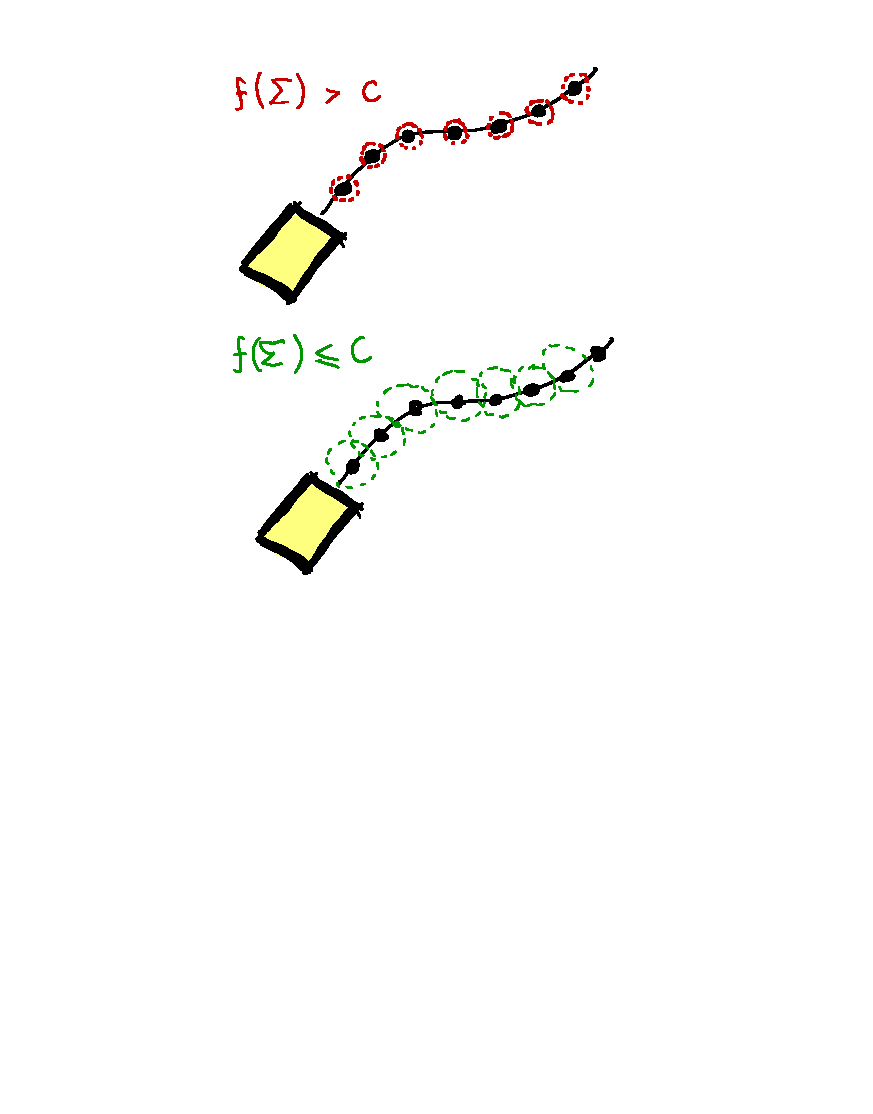
\includegraphics[clip, trim=0cm 8cm 0cm 1cm, width = 0.75\textwidth]{Thing.pdf}
%    \caption{Relaxing the Ridgeback pose constraints depending on the localization covariance, lower covariance gives more space to optimize for manipulability}
%    \label{fig:somthing}
%\end{figure}
\subsection{The SQP algorithm}
Sequential convex optimization optimization can be tackled using sequential quadratic programming (SQP) \citep{schulman2013finding, xu2010two}, a powerful algorithm which repeatedly constructs and minimizes a convex approximation of the problem $\tilde{P}$ until constraints are satisfied.
\paragraph*{Initialize}
The cost and constraint functions can be picked at runtime or compile time.
An advantage of picking the functions at runtime lies in having the ability to parametrized generic versions of commonly used constraints such as collision avoidance or field of view maintenance.
\paragraph*{Convexify}
For each point in the desired trajectory and the penalty value $\mu$, we form convex cost and constraint functions at the operating point.
The cost function is convexified to a second-order approximation while the constraints are linearized at the current configuration.
\paragraph*{Minimize}
The convexified problems are minimized, where the parameter values being considered are subject to the trust region $\delta$.
This prevents the minimization process from taking large steps when the changes in the convex cost and constraint models do not reflect the changes in the non-linear models to a sufficient degree.
\paragraph*{Trust Region}
At each iteration of the innermost for loop, a trust region $\delta$ for the QP problem is updated depending on how well the change proposed by the minimization algorithm translates to the change in non-linear models of the cost and constraint functions.
If the change is deemed sufficient, the step size for the next iteration is increased by modifying the parameter search area of the optimization algorithm.
\paragraph*{Check constraints} 
Once the convexify loop converges (the changes in $q$ become sufficiently small) or reaches a maximum number of iterations, the result is checked against constraints.
If the constraints are satisfied, the algorithm concludes.
Otherwise, the penalty $\mu$ is increased (usually by a degree of magnitude) and the algorithm is repeated.

\begin{algorithm}[h]
 \KwData{$q_{init}\,$}
 \KwResult{Configuration $q$ satisfying $f,g,h$}
 $f,g,h \leftarrow$ Initialize()\tcc*[r]{Initialize problem}
 \For{PenaltyIteration = 1,2,\, \dots}{
  \For{ConvexifyIteration = 1,2,\, \dots}{
  $\tilde{f}, \tilde{g}, \tilde{h} \gets$ Convexify($f,g,h$)\tcc*[r]{convexify problem}
   \For{TrustRegionIteration = 1,2,\, \dots }{
   $\begin{array}{rl} \min\limits_{q} & G(\tilde{f}, \tilde{g}, \tilde{h}) \\
    \mbox{s.t.} & q \in \left[q - \delta, q + \delta \right] \end{array}$\tcc*[r]{minimize}
   \If{TrueImprove / ModelImprove $\ge$ c}{
   $\delta \gets \tau^+ \delta$\tcc*[r]{expand trust region and proceed}
   \textbf{break}\;
   }
   $\delta \gets \tau^- \delta$\tcc*[r]{shrink trust region and repeat}
 }
   \If{Converged()}{
   \textbf{break}\;
   }
 }
  \eIf(\tcc*[h]{Check nonlinear constraints}){$SatisfiesConstraints$}{
 \textbf{return} $q$\;
 }{
 $\mu = k*\mu$\;
 }
 }
 \caption{The SQP algorithm}
 \label{algorithm:sqp}
\end{algorithm}










\chapter{Software architecture}
With the theoretical framework for state estimation and motion planning established in \autoref{chapter:State estimation} and \autoref{chapter:motion planning}, this chapter describes the software implementation of these ideas.
Developing code that is intuitively structured is key in a research context, where it is often maintained and expanded by multiple parties.
Maintaining a heavily tested core code-base which allows modular drop-in components for high level functions is an optimal development strategy for such cases.
Such a structure expedites testing and data gathering procedures, as it enables quick start-up, user safety and damage prevention.

In \autoref{section:overview} development considerations are explained in more detail and a high-level overview of the software architecture is presented.
Next, in \autoref{section:code state estimation} and \autoref{section:code motion planning} state estimation and motion planning pipelines are presented in more detail.%, focusing on the modularity aspect.
Lastly, \autoref{section:control} describes the control pipeline that relays user commands to the API and internal control loops. %%Due to closed-source control code being used in the robots internally, we omit the details of the algorithms themselves in lieu of explaining interfacing strategies with the low-level APIs.

\section{Overview}\label{section:overview}
Developing software for a complex system such as the Thing mobile manipulator is a time-consuming process, as each change requires extensive testing before it can be applied safely.
Aside from maintaining a strict version control strategy with tools such as \textit{git}, the developer needs to have an idea of what interaction a given change can have with the rest of the code-base as it is often inefficient to test every change in detail.
Structuring the code in a way that decouples most of the heavily-tested core functionalities from specific user tasks is of great importance since it helps the developer maintain an idea of what certain changes can affect.

The testing procedure on the real robot suffers from a high set-up cost, which can be reduced by having start-up procedures stored in the form of ROS launch files.
Having a simulation that reasonably models the robots behaviour also expedites testing, as some concepts remain largely unaffected by dynamic effects occurring in reality.
Furthermore, platform-agnostic code is maintained, meaning that the software does not differentiate between the simulated and real systems, drastically reducing implementation time.
\subsection{Architecture}
The network-based nature of ROS systems allows a distributed software architecture.
This enables keeping real-time dependent functionalities on the robot while running high level algorithms on a separate machine.
Specifically, the control algorithms implemented in \verb|ros_control| interface with the local UR10 and Ridgeback drivers and are ran on the robot's local machine which acts as a server.
Task-specific programs are ran on a separate machine or client which connects to the Thing's ROS core via WiFi or ethernet.
\begin{figure}
\includestandalone[width=\textwidth]{slike/software_tikz}
\caption{Overview of the software architecture. White rounded rectangles represent ROS packages, while cross-hatched rectangles represent individual libraries/headers/executables.}
\label{fig:overview}
\end{figure} 

\subsubsection{Client}
\autoref{fig:overview} shows how the \verb|thing_control| package forms a robust core of the code-base.
It acts as a central node which processes trajectories and commands sent by the user, which includes:
\begin{itemize}
  \item Receiving and processing data streams from the robot
  \item Sending joint-level commands to the lower-level control architecture
  \item Processing (solving) Cartesian trajectories sent by the user
  \item Monitoring incoming data streams and implementing security procedures
\end{itemize}
Receiving and sending data is done through the ROS topic interface; subscribers fetch structured data from network locations called topics which are populated using publishers.

At compile time, the user can choose a motion planner developed specifically for the Thing mobile manipulator.
These planners inherit from a core part of the code-base, the \verb|thing_kinematics| library.
This library contains the common mathematical framework for the motion planners as well as various useful kinematics functions:
\begin{itemize}
  \item Forward kinematics and Jacobian functions
  \item Pose error calculations
  \item Angle representation conversions
  \item Various matrix operations
\end{itemize}
Keeping this part of code in library form allows for easy transfer of these useful functionalities to other packages.
The motion planners (also referred to as \textit{solvers}) represent different approaches to the problem of solving a given Cartesian trajectory.
Both the methods presented in \autoref{section:task priority}, \autoref{section:sqp} are implemented as motion planning libraries.

\subsubsection{Server}
The computer located on the robot itself or server maintains the control and estimation pipeline on the robot and takes care of publishing the current state and status to the network.

Direct communication with the base and manipulator is achieved through their respective APIs, but in order to connect these libraries to our networked software structure the \verb|ros_control| package is used. 
It provides a valuable set of tools that abstract the notion of a robot interface and enable quick and easy integration of APIs into ROS-based system architectures.

The transforms representing all of the chains located in the robots URDF\footnote{\textit{Unified Robot Description Format} - Standard file format used for semantic robot descriptions.} file resulting from state estimation are published thorugh the \verb|robot_state_publisher| package. The package publishes the transforms in the form of standardized \verb|\tf| ROS messages.
The package is launched on the robot's local machine since the standardized structure of the control pipeline relies on the transforms published by this package.

\section{State estimation}\label{section:code state estimation}
The EKF algorithm described in \autoref{section:Localization} is available as a component of the \verb|robot_localization| package \citep{MooreStouchKeneralizedEkf2014}.
This package fuses odometry estimates provided by various sources, ideally resulting in a higher-accuracy estimate.
The estimates need to be published to a ROS topic in the form of a \verb|nav_msgs/odometry| message.
Each state estimation node in \verb|robot_localization| begins estimating the vehicle’s state as soon as it receives a single measurement. If there is a holiday in the sensor data (i.e., a long period in which no data is received), the filter will continue to estimate the robot’s state via an internal motion model.

\section{Motion planning}\label{section:code motion planning}
Two motion planning algorithm have been developed, one implementing the \textit{task-priority} (\autoref{section:task priority}) scheme and the other implementing the scheme in \eqref{mnptik_2} via the SQP (\autoref{section:sqp}) algorithm.

Unifying the implementations is a common linear algebra framework, the Eigen3\footnote{http://eigen.tuxfamily.org/index.php?title=Main\_ Page} library.
The Eigen3 library is a powerful linear algebra toolbox capable of handling a vast array of dense and sparse matrix calculations.
It is also templated and heavily optimized for reducing redundant value copying and memory management, making it the basis of many algorithm implementations across a range of fields.

\subsection{Task-priority}
Unlike the SQP implementations, task-priority is implemented using only the Eigen3 and C++ standard libraries.
It relies on \textit{singular value filtering} \eqref{eq:svf} and the \textit{selectively damped least squares} \eqref{eq:sdp} formulation to maintain numeric stability in the pseudoinverse operation.
These functions have been developed from scratch in highly abstracted template form for the purposes of this work and are publicly available.

\subsection{Sequential convex optimization}
Implementation of the sequential convex optimization algorithm is done using Google Ceres\footnote{http://ceres-solver.org/} solver as the underlying convex optimization subprogram.
The objective and convexified constraint functions are implemented as classes in order to be compatible with the solver.
Ceres is configured to run using the Levenberg-Marquardt trust-region strategy with the Broyden–Fletcher–Goldfarb–Shanno algorithm being used for performing line search.

\section{Control}\label{section:control}
The underlying control architecture of the Thing mobile manipulator relies heavily on the internal APIs of both the UR10 and Ridgeback.
Thus, the main challenge in implementing the software architecture lies integration of control inputs and outputs rather than parametrization of a control loop.
The \verb|ros_control| package functions as an integration tool for robot APIs into the networked structure of ROS-based systems.
\begin{figure}
\centering
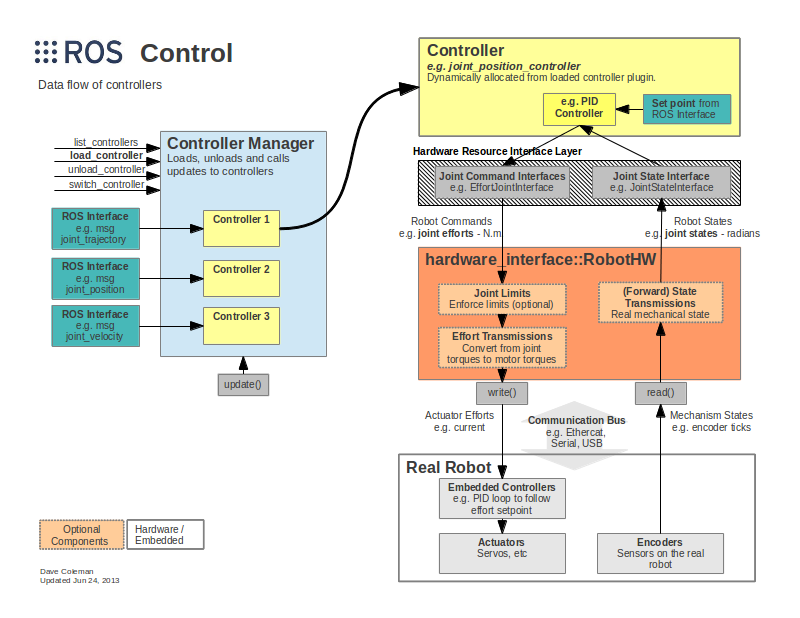
\includegraphics[width=0.9\textwidth]{ros_control}
\caption{Scheme of ros\_ control functionalities}
\label{fig:ros control}
\end{figure}
The \verb|hardware_interface| (\autoref{fig:ros control}) class is used to wrap the read and write methods of the respective APIs in to function handles. 
These handles can then be used by a selection of controllers within the package to either forward commands or implement a control loop.
A ros controller has many types and is configured using a yaml file. 
Depending on the interface, this controller will forward commands or actually control the signal using tunable PID parameters.
Additionally, we use the joint trajectory controllers which can handle and interpolate multiple timed trajectory points.



\chapter{Results}
This chapter covers the results of the presented state estimation and motion planning approaches.
Since motion planning was considered on a purely kinematic level, it is extensively tested in both simulation and on the real robot.
State estimation testing proved more difficult as dynamic effects such as slip are not easily simulated.
For this reason state estimation was only explored in data sets collected from the real robot.
\begin{figure*}[h]
    \centering
    \begin{subfigure}[t]{0.45\textwidth}
        \includegraphics[trim={35cm 0cm 0cm 0cm},clip,width=\textwidth]{lidar_test1}
        \caption{Tests in the VICON laboratory}
        \label{figure:VICONtest}
    \end{subfigure}
    \begin{subfigure}[t]{0.45\textwidth}
        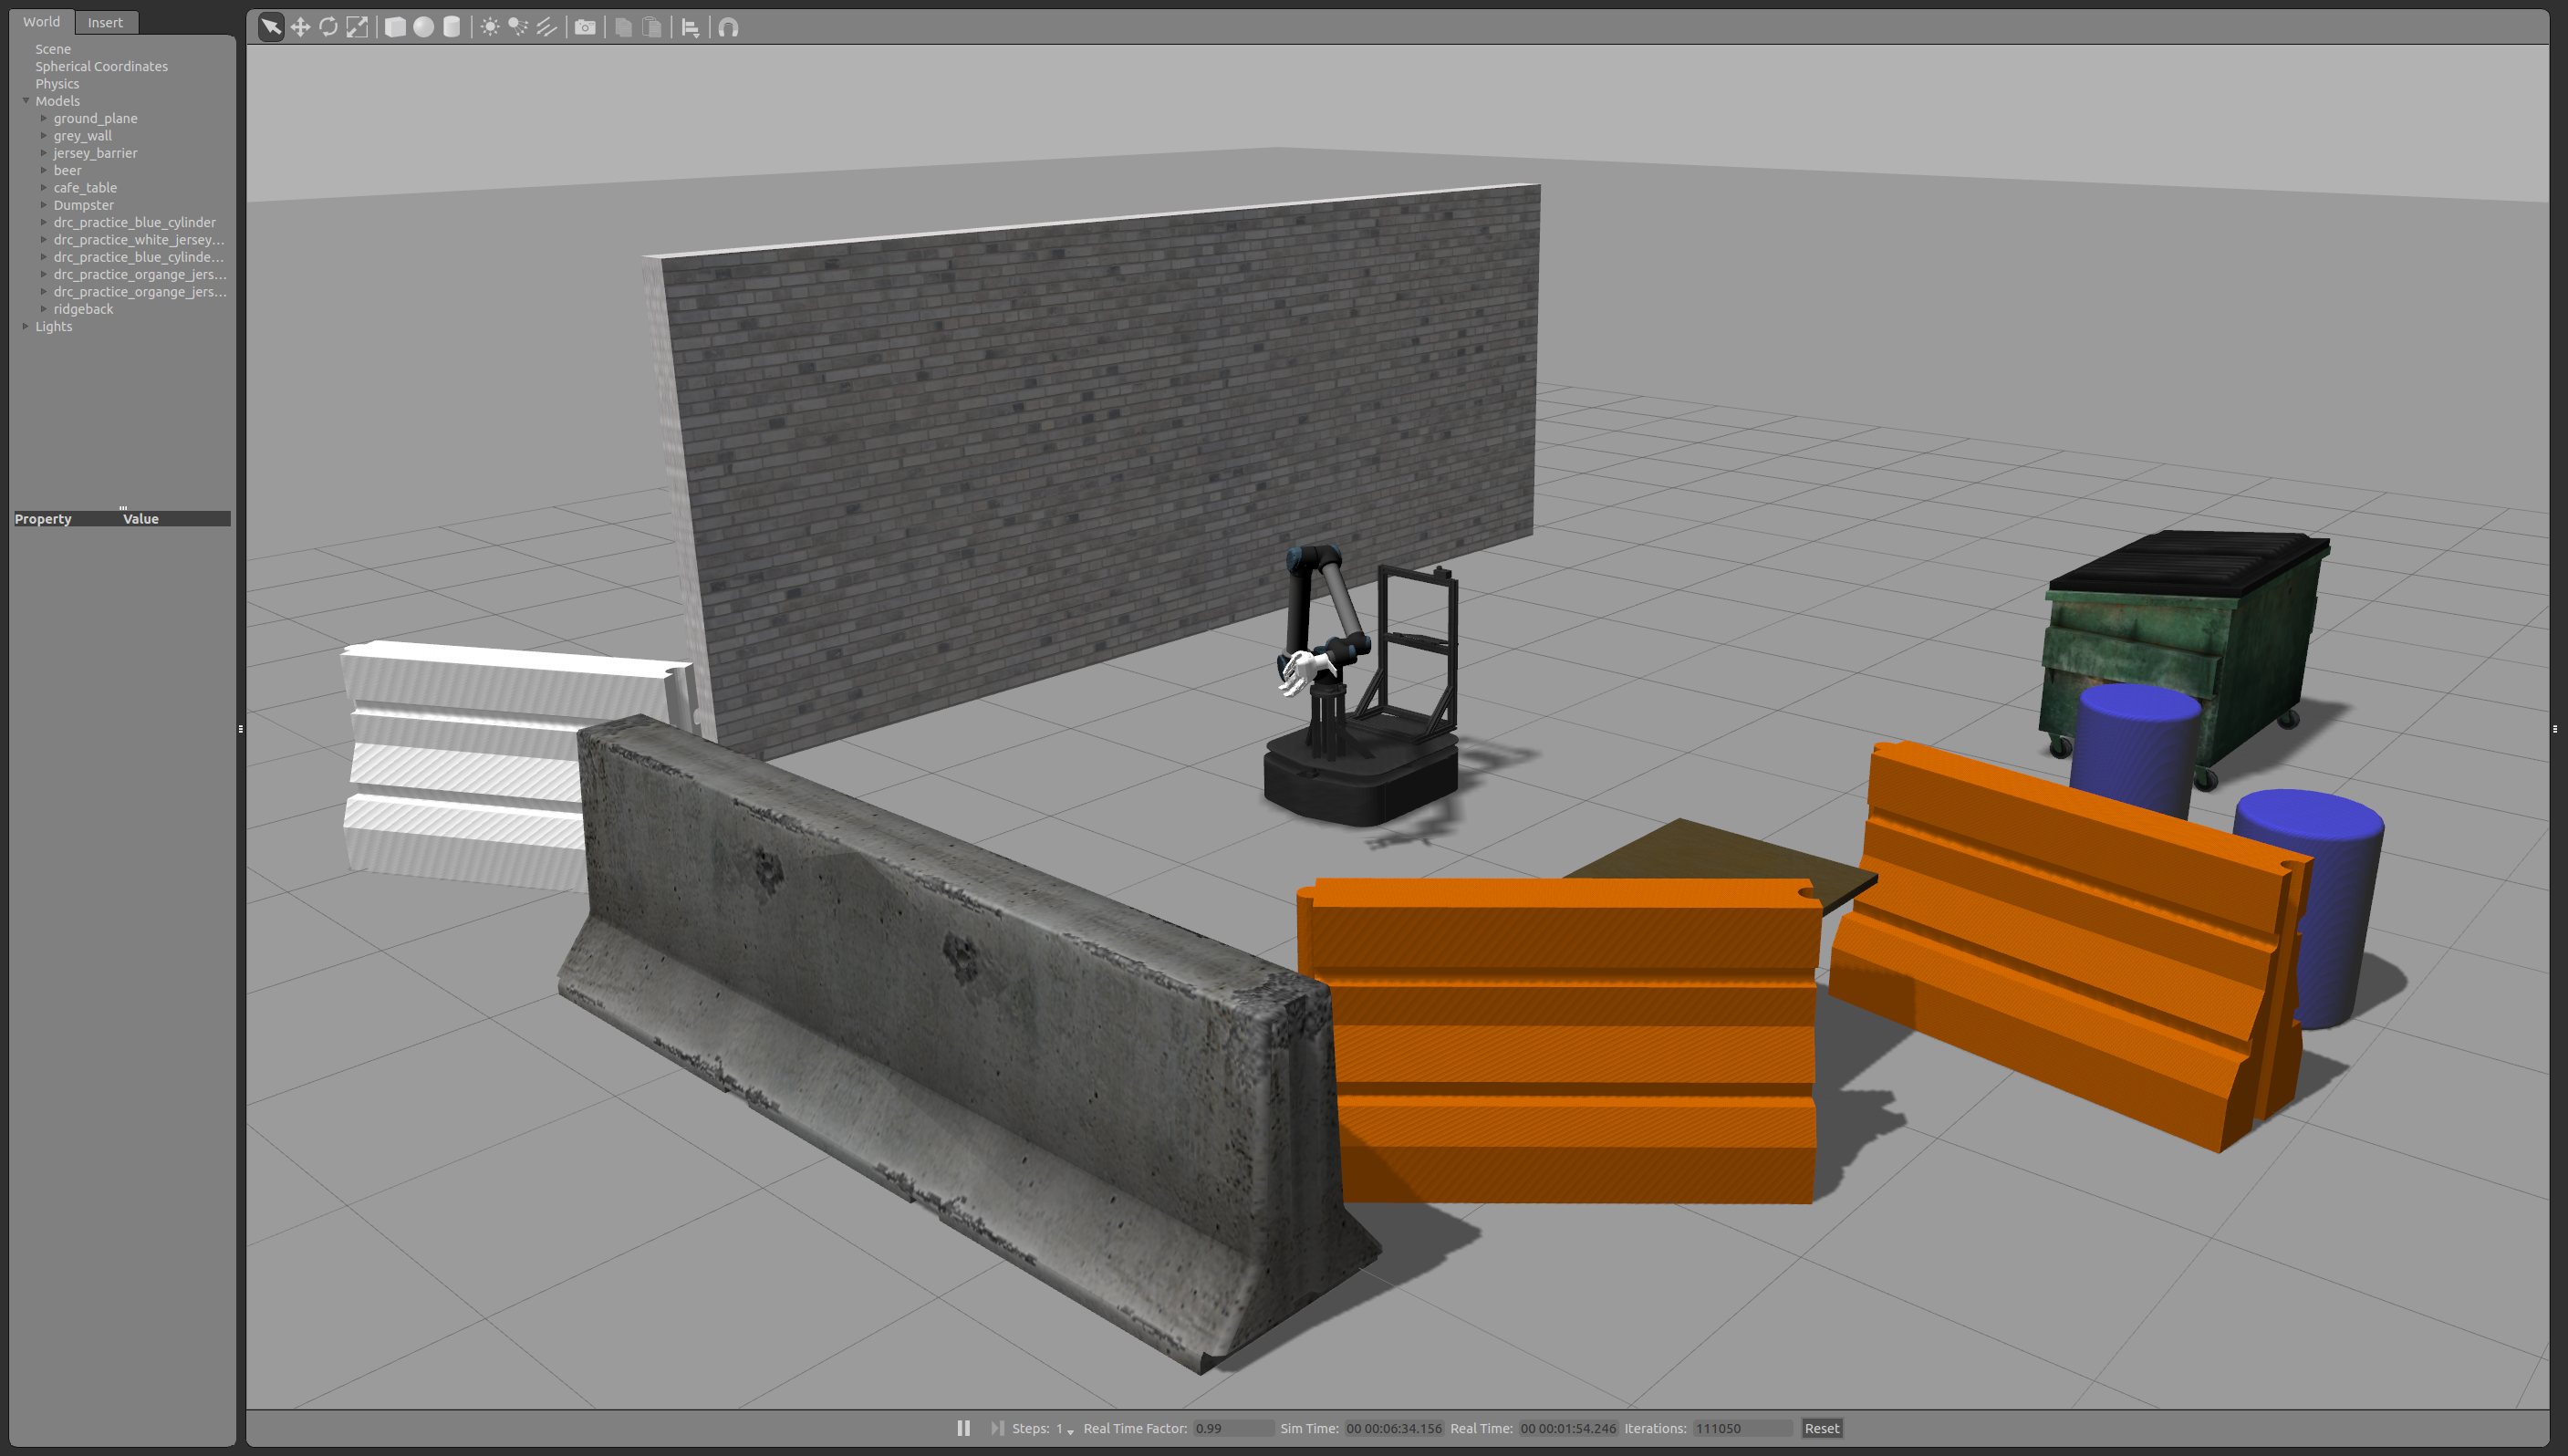
\includegraphics[trim={25cm 2.5cm 10cm 8cm},clip,width=\textwidth]{gazebo_screenshot1}
        \caption{Simulation testing setup}
        \label{figure:simulationtest}
    \end{subfigure}
    \caption{Example of some real and simulated test setups.}\label{fig:resultsphotos}
\end{figure*}
Localization tests were performed in the VICON laboratory at the University of Toronto Institute for Aerospace Studies (UTIAS).
VICON is a commercial motion capture system ideal for the purposes of setting ground-truth values for state estimation tests and is used as such in all of the tests in this chapter. 
\section{Simulation}
The Thing mobile manipulator is simulated using the Gazebo simulator.
Aside from being open-source, the main advantage of this simulator is that it is fully integrated within the ROS ecosystem.
Furthermore, the \verb|ros_control| controllers used on the actual robot are also integrated in the Gazebo simulation, expediting the implementation procedure.

\section{Real}
%\begin{figure}[h]
%\centering
%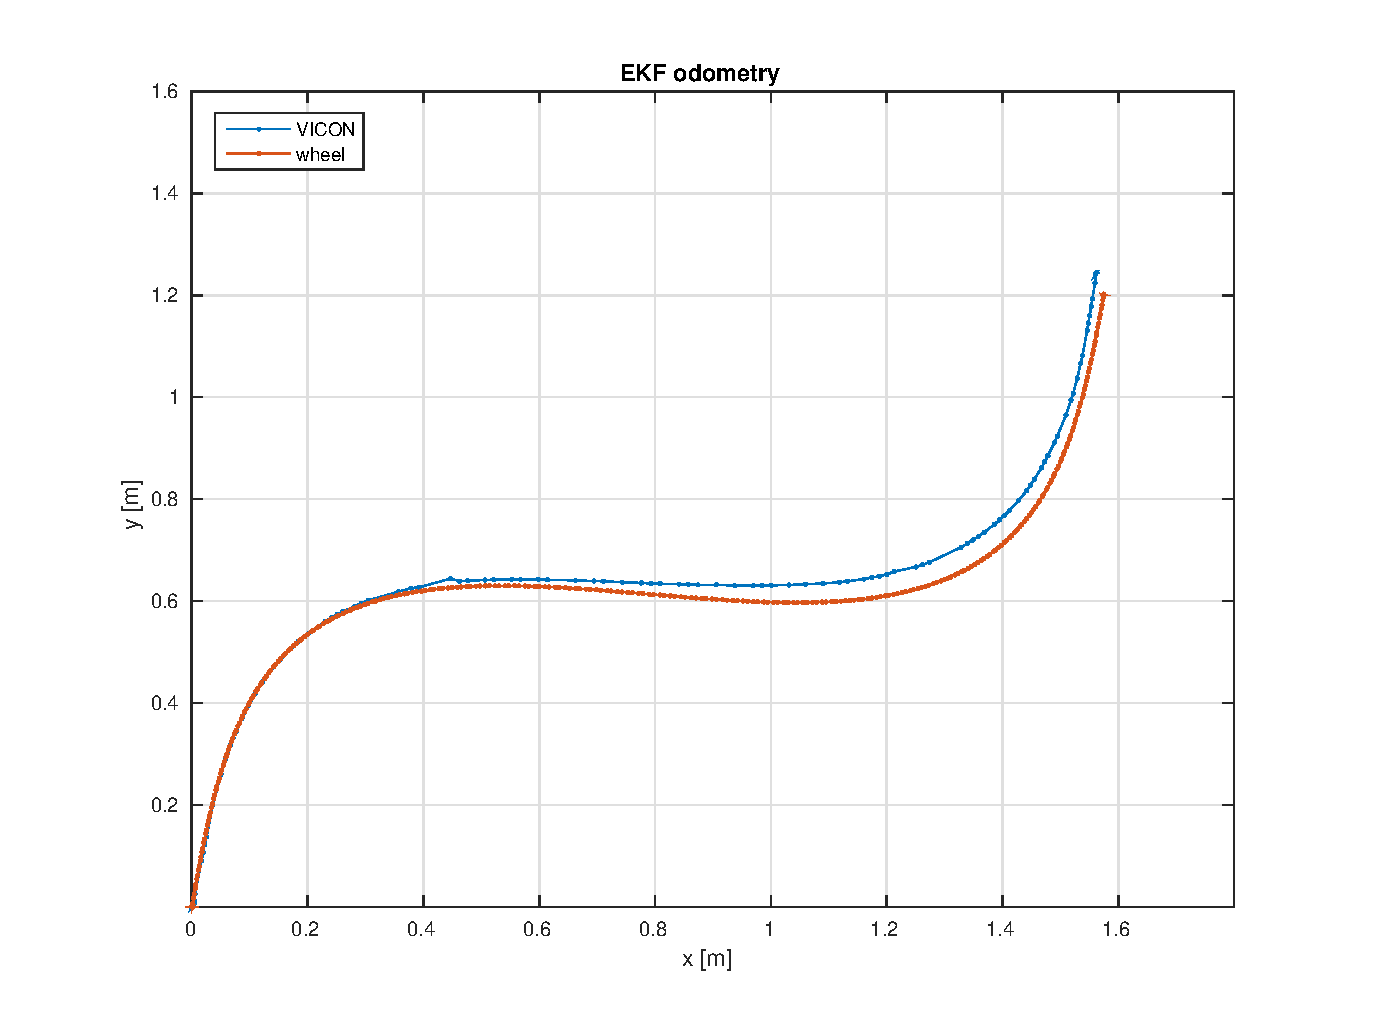
\includegraphics[width=.75\textwidth]{localization1}
%\caption{Simulated localization}
%\end{figure}

\subsection{Localization results}
\autoref{fig:ekf_localization} shows the results of base localization on  a dataset consisting of manual Ridgeback movement inputs.
Two variants are compared: the first variant  uses an EKF to achieve fusion of both the wheel and LIDAR odometry, the second variant integrates wheel odometry alone using the EKF only to account for measurement noise.
\begin{figure}[h]
\centering
% This file was created by matlab2tikz.
%
%The latest updates can be retrieved from
%  http://www.mathworks.com/matlabcentral/fileexchange/22022-matlab2tikz-matlab2tikz
%where you can also make suggestions and rate matlab2tikz.
%
\definecolor{mycolor1}{RGB}{ 38, 166, 91}%
\definecolor{mycolor2}{rgb}{0.85000,0.32500,0.09800}%
\definecolor{mycolor3}{RGB}{75, 119, 190}%
%
\begin{tikzpicture}

\begin{axis}[%
width=4.682in,
height=3.6in,
at={(0.785in,0.486in)},
scale only axis,
xmin=-0.5,
xmax=1,
xlabel style={font=\color{white!15!black}},
xlabel={x [m]},
ymin=-0.2,
ymax=1.4,
ylabel style={font=\color{white!15!black}},
ylabel={y [m]},
axis background/.style={fill=white},
%title style={font=\bfseries},
%title={EKF odometry},
axis x line*=bottom,
axis y line*=left,
xmajorgrids,
ymajorgrids,
zmajorgrids,
legend style={at={(0.156,0.779)}, anchor=south west, legend cell align=left, align=left, draw=white!15!black}
]
\addplot [color=mycolor1,line width=1pt]
  table[row sep=crcr]{%
6.28612846153842e-05	2.51965475542154e-05\\
9.77225408177462e-05	-4.01509786358833e-05\\
7.62616093439306e-05	0.000178726628546844\\
4.89661012158527e-05	0.000150750214168827\\
5.47246500886486e-05	0.000255191013130276\\
0.000104783497418263	0.000142188469222759\\
4.19614936356394e-05	0.000118277191405725\\
0.000162329007018028	0.000130311228559624\\
-3.10309197674163e-05	0.000242354947985898\\
0.000185622277808641	5.24663669910774e-05\\
2.81565392624208e-05	4.14027649921628e-05\\
-5.74593650044114e-05	4.24448394022031e-05\\
0.000144371103512564	5.89668849284991e-05\\
7.49571222413564e-05	2.08701473315559e-05\\
-4.72816011319044e-05	6.19806260526989e-05\\
0.000181988585342019	0.000103724692286838\\
0.000261095932502974	0.000205889236927922\\
0.000224283039116584	3.22314725013928e-05\\
6.67830391812563e-05	0.000188861252775091\\
-1.11410436451076e-05	9.8063689583136e-05\\
4.43446249952101e-05	0.000173698551394874\\
0.000151461057912715	1.57223867234962e-05\\
0.000142278028875446	5.76500301022187e-06\\
6.41867484418163e-06	4.56375516730417e-05\\
-2.6571682340687e-06	0.000124330662335012\\
0.000119134311348884	-6.38456661988807e-06\\
4.66601860236518e-05	8.84011674792268e-05\\
0.000231719014463221	-2.30754518951853e-05\\
6.65146661682839e-05	9.17372675138112e-05\\
0.000134330992549003	0.000104930983901644\\
0.000382238938425219	0.000306891615147326\\
0.000326967238680267	0.000318339466775744\\
0.000183388045270405	-2.87879080084902e-05\\
5.11818577334511e-05	0.000182742227525068\\
-8.36664870218079e-05	-2.37427709747218e-05\\
0.000205209872296878	8.66704182442418e-05\\
8.04156316759758e-05	0.000168942249172202\\
9.44069841287143e-05	-3.10635113244667e-05\\
0.000220786733376263	5.80449024394636e-05\\
0.000124030199634945	0.00011300711365296\\
0.00017132949968101	1.5434922280011e-06\\
0.000148671201525542	1.42399322252407e-05\\
0.000112275595636216	0.000152815832092201\\
0.000219006178388298	0.000334346698493776\\
0.00014265948688872	0.000127364052676798\\
0.000221768792342064	6.75067216399372e-05\\
4.01303536616271e-05	-8.34901528188603e-05\\
0.000259976569730348	0.000268255120615415\\
0.00021409894653298	4.81556634950447e-05\\
7.44519193913856e-05	-4.46168998019386e-05\\
3.92459505209192e-05	1.70492931452909e-05\\
0.0002661073566739	0.000148951107085293\\
5.67945216248117e-05	6.4491215300333e-05\\
3.09826222526927e-06	2.93349529227743e-05\\
0.000289728430289668	0.0001763313082455\\
0.000243114697029402	0.000395805360883461\\
8.5416146125783e-05	1.16630821021813e-06\\
0.000258814208288105	0.000168569948764727\\
0.000201431214361725	-5.20678231839822e-05\\
0.000100855307859832	0.000203797129412445\\
0.00017097473094458	2.01616696676732e-06\\
0.000290552198555553	0.000125288183253733\\
0.000277693047563546	0.000147905668627699\\
7.94981380952131e-05	0.00028708544150205\\
3.92327491470987e-05	0.000211183852324021\\
0.000291049824429783	7.38167974749931e-05\\
0.00109654124687748	-4.93013868643616e-05\\
0.0028660817437496	-0.000450469199983969\\
0.00714765543668146	-0.000666093254271277\\
0.0128116852730542	-0.0012495525158881\\
0.018447610864353	-0.00173587459017455\\
0.0215103988082662	-0.00193883318969383\\
0.0243886881786806	-0.00201261076049843\\
0.0309046261856262	-0.00293531001783399\\
0.0439019670059303	-0.00463928200667788\\
0.0493055712800541	-0.00509473904217238\\
0.0545511478563844	-0.00555474185610454\\
0.0592906074463817	-0.00548063919813373\\
0.0652461426101595	-0.00650205738428725\\
0.0746681023916896	-0.00727582762807115\\
0.0798863859000749	-0.00762279626649828\\
0.0898239396196476	-0.00902578000469702\\
0.0998993162370925	-0.00976308063195513\\
0.105342295247501	-0.0104104890560966\\
0.110527342507382	-0.010888990520354\\
0.131413636661927	-0.0128943089740079\\
0.138602734121672	-0.0136133475007029\\
0.147371925939373	-0.0148915994555338\\
0.163990256367886	-0.0166907805032064\\
0.1785072158231	-0.0178054257668784\\
0.185865128419791	-0.0182707603328307\\
0.193277502870887	-0.0193694114311594\\
0.207853444279779	-0.0210236428110017\\
0.222610314465006	-0.0223997407193949\\
0.229889568458062	-0.0238343127918324\\
0.239550974364359	-0.0240518740869544\\
0.267957941195967	-0.0276395128367998\\
0.27586049590226	-0.0282516994079154\\
0.283151956721414	-0.0290681639273232\\
0.297519205341832	-0.029928943875495\\
0.312832253540154	-0.0311612088270239\\
0.32103933687439	-0.0319173728600923\\
0.328693927573642	-0.0326960262450458\\
0.356356339077932	-0.0354861676591697\\
0.36020379298985	-0.0353404745629102\\
0.360162218620425	-0.0350927649959414\\
0.359240938286625	-0.0350152329292208\\
0.358460635527793	-0.0349008360095523\\
0.358112211121691	-0.034644715908509\\
0.357291788732297	-0.0349220991591322\\
0.352207838088347	-0.0342737368346668\\
0.33866589131342	-0.032586947064796\\
0.334435300452298	-0.0320559708667695\\
0.320877521661443	-0.0310089745152508\\
0.317583560038716	-0.0304811937542549\\
0.314275344007809	-0.03074943039832\\
0.311107024260542	-0.0297976220802226\\
0.307461897951356	-0.0295897798820561\\
0.298834574841521	-0.0288914148057989\\
0.295089517818131	-0.0281766620032286\\
0.291121358656109	-0.0279271158743403\\
0.279558569534313	-0.0264942292772195\\
0.276311341491443	-0.0262351450781735\\
0.26932155982021	-0.025821885498458\\
0.265620394528363	-0.0260296162609331\\
0.262195222216112	-0.0260399540571\\
0.253549089256167	-0.0255310621543474\\
0.248978688040166	-0.0258274022503611\\
0.24513023689414	-0.0250788872342128\\
0.241433809968211	-0.024133512155674\\
0.238698868964991	-0.0236696535001846\\
0.227895000481366	-0.0242525325962365\\
0.225195862310723	-0.0236003909046234\\
0.22637950338847	-0.0233671157051121\\
0.229077867295791	-0.0224954008282634\\
0.231943944475836	-0.0231676798448991\\
0.236324184839091	-0.0237314395796132\\
0.246690837095513	-0.0232244652079742\\
0.262048043659934	-0.0223356464207201\\
0.271301131123779	-0.022369245767995\\
0.2808919474571	-0.0222727945603568\\
0.297833229831412	-0.0224890164830636\\
0.313130648247603	-0.0230117188701593\\
0.32137902332886	-0.0237865270945227\\
0.329830909730791	-0.0249795658017836\\
0.345872263597224	-0.0266158989637058\\
0.361507961772114	-0.0299681026760141\\
0.36946095242451	-0.0327796677923437\\
0.377587663003732	-0.0354875505367323\\
0.393797896540926	-0.0402154516007968\\
0.406935153235934	-0.0449893519634026\\
0.410238298345305	-0.0449570398539046\\
0.40894470246925	-0.0440762247676562\\
0.407126949216951	-0.0431884667064523\\
0.405726931837354	-0.0436401493665594\\
0.405648540746113	-0.0430022632449594\\
0.401941474796102	-0.0414930351491914\\
0.392718277100795	-0.0395884066657712\\
0.384890596796872	-0.0380881501856113\\
0.381399408212141	-0.0361711680517003\\
0.377450826221075	-0.0347018499647272\\
0.367941583233143	-0.0324685663696388\\
0.352469610245219	-0.029543472554611\\
0.347075632549718	-0.0294527935420321\\
0.341013510038627	-0.0288372577087528\\
0.327972180272092	-0.0276152838628177\\
0.316821053495755	-0.0265702707342032\\
0.310032701296529	-0.025700078513333\\
0.303834130356767	-0.0256107452961515\\
0.297446144943135	-0.0250389112475715\\
0.291713905049783	-0.024974309070454\\
0.279565072590215	-0.0246595304191865\\
0.273709127950952	-0.0247580700960197\\
0.267203905257143	-0.0251931483264937\\
0.254271353075818	-0.0259386010769646\\
0.246859691243217	-0.0266919727070054\\
0.240808742577596	-0.0277062249323859\\
0.236466423098962	-0.0281944557156626\\
0.229938689987002	-0.0296395612056711\\
0.22361288131531	-0.0304270145925235\\
0.218172840477181	-0.0316256876050436\\
0.206506394025418	-0.0338384987830647\\
0.200835736950277	-0.0350608924653358\\
0.195169462599472	-0.0365117532473909\\
0.186792382354045	-0.038597583023121\\
0.187703425812109	-0.0379724139278065\\
0.188679983855162	-0.0367769529366585\\
0.189840149287617	-0.0361374939021684\\
0.193900123973449	-0.0368446681294739\\
0.210018637310082	-0.0352460320390588\\
0.219857084123977	-0.0332009128044669\\
0.23125986974507	-0.0310327276385177\\
0.265045725003034	-0.0231639484095168\\
0.275271395154172	-0.020015203333321\\
0.286770242090854	-0.0171560559261165\\
0.298071082343279	-0.0155909216032843\\
0.319456960123189	-0.0104137755773667\\
0.340457965234237	-0.00637518302732999\\
0.352116187803144	-0.00415237290182999\\
0.363077615886327	-0.00167934742893039\\
0.384615488624157	0.00291597376550863\\
0.406072441799826	0.00742843364762424\\
0.417477903560681	0.00956632047031451\\
0.428608089639532	0.0114030551637584\\
0.439326701666296	0.0141632696796062\\
0.44968512246443	0.0161802196041737\\
0.462239226250103	0.0186071972435935\\
0.471706195147192	0.0202666192225452\\
0.482588144788082	0.0226068671179561\\
0.493757878500598	0.0248383283056608\\
0.536476194225572	0.0336449299069055\\
0.547398506574837	0.03573342605077\\
0.558816118638957	0.0381115726436542\\
0.57005936454958	0.0401014676782034\\
0.58016814110501	0.0426950869239881\\
0.599648351283727	0.0466631942568587\\
0.605600122065452	0.047573026972397\\
0.608399687109754	0.0481131121783425\\
0.608928213522907	0.0488031995320393\\
0.60757436763463	0.04840225450788\\
0.60367486176951	0.0473999614973968\\
0.59685136143639	0.0456180849302568\\
0.589270185933453	0.04401795183525\\
0.582386227898013	0.0424577686920418\\
0.567695788384921	0.0398719247574827\\
0.5594586508613	0.0385499406565191\\
0.550570494561758	0.036775138066565\\
0.534216000928696	0.033262240799959\\
0.518431824563679	0.0301055218641736\\
0.508500490234295	0.0284370160566602\\
0.497180601989359	0.0264897930418665\\
0.473063667859536	0.0214339209623675\\
0.452193185077296	0.016964629862161\\
0.440935172694454	0.0152752915424393\\
0.427279580208734	0.0121574268813027\\
0.407738447882077	0.00799450799212892\\
0.386202038157625	0.0022441404867888\\
0.375119321961986	-0.00162243065568789\\
0.364601827476025	-0.00600965549602994\\
0.344607618898676	-0.013961899886629\\
0.31247624898362	-0.0249739620087866\\
0.301869902487713	-0.0304988658797771\\
0.261869663051136	-0.0478502631773903\\
0.251111877461805	-0.0528539753870355\\
0.240861121727573	-0.0591498222491548\\
0.208795250233301	-0.0771424515886309\\
0.205046251924917	-0.0787427683394001\\
0.203029288370556	-0.0803711310296449\\
0.201744913628055	-0.0812423529269169\\
0.201732988976083	-0.0815073845319842\\
0.20254438374038	-0.0815163533688026\\
0.206757629342819	-0.0793349176747538\\
0.214638257467618	-0.0751344331904739\\
0.233453614910614	-0.0657630005716207\\
0.252365251857677	-0.0579497369453807\\
0.266100100346191	-0.0513929255375459\\
0.279441438892766	-0.0431386400143316\\
0.292285259533821	-0.034883610603373\\
0.303361930907021	-0.0268104521055046\\
0.327570289707603	-0.012761669490324\\
0.340705802806785	-0.00552900780706243\\
0.353366541770234	0.00218343383246282\\
0.377240226625216	0.0160117818501072\\
0.402116098333506	0.0313270819578191\\
0.415012298844453	0.0381769701523994\\
0.427812686264559	0.0458449177157612\\
0.451601615646894	0.0605007622732265\\
0.474241270700103	0.0780156589614603\\
0.48634427639943	0.0877896375682028\\
0.498297646930422	0.0991226750207532\\
0.520253088325356	0.120462445345808\\
0.538026045702565	0.146648638254801\\
0.546679104556991	0.160366114374255\\
0.553793420888135	0.176082833982487\\
0.558896883378101	0.19437644205407\\
0.561719824884966	0.210807647861799\\
0.5613404057467	0.242659708179781\\
0.556975664223858	0.259145087182495\\
0.534481449714663	0.294080894166124\\
0.515216802415398	0.31872500592624\\
0.504243060249819	0.332867320792247\\
0.493363224044649	0.345718737229108\\
0.47112983821364	0.371358096614544\\
0.445692664045159	0.393226859769715\\
0.430196532841266	0.40519852434241\\
0.414926710123225	0.41550738158004\\
0.398949092484096	0.425050993037819\\
0.382947864493969	0.432246302899374\\
0.347350221983722	0.443933998236706\\
0.328447176297426	0.449329491908315\\
0.308919455818869	0.449887999333952\\
0.289182534513868	0.450094304854\\
0.271526973101733	0.449050011023202\\
0.237253379943222	0.440558404383752\\
0.222197908678727	0.432701171070578\\
0.209358593051554	0.423175118923385\\
0.197292819252611	0.412829022255704\\
0.185024096724126	0.402045782739784\\
0.172903762450214	0.390677880981997\\
0.156332379654119	0.37615694998703\\
0.143427039321521	0.365451326062312\\
0.128581893979577	0.353755781713909\\
0.113236586746203	0.3396210760672\\
0.092194370851399	0.316410918330267\\
0.08246617831848	0.302967174077119\\
0.0732899790504377	0.289967159661492\\
0.0625982360922262	0.262773241903605\\
0.0578691847010801	0.239602589792886\\
0.0570460615326268	0.226362201758653\\
0.0557461385945047	0.213368868527498\\
0.0547557201283617	0.201296554279208\\
0.0541826914491287	0.189466175304412\\
0.0555218694432463	0.164871034835694\\
0.0583685066584095	0.152337439572136\\
0.061760500743243	0.138656484276776\\
0.0661100701608938	0.125300898775631\\
0.0837545077325915	0.0899233878360403\\
0.0905418117374267	0.0779254985138805\\
0.0990027515275739	0.0670303229920266\\
0.135465842265411	0.0220960232980478\\
0.14564758921688	0.00998428622958096\\
0.15623621535537	-0.00167920349321957\\
0.178355809522777	-0.0210007125916101\\
0.201688283235066	-0.0399826588605275\\
0.214994124302581	-0.0502198647159798\\
0.228661815801369	-0.0602431525665456\\
0.242858351602362	-0.0689919980488917\\
0.285788443371086	-0.0907192041316134\\
0.301049084195734	-0.0981703783109016\\
0.317109453273701	-0.104620042988576\\
0.350434338556555	-0.110069194434453\\
0.384617076469293	-0.110134234782541\\
0.402835287696119	-0.10714583474708\\
0.421729364712543	-0.103633465678308\\
0.456971500651055	-0.0939392369232507\\
0.509376728297224	-0.0790874541215075\\
0.526252158263983	-0.0733957198028448\\
0.556423823139245	-0.0603906553207223\\
0.58290220742624	-0.0415540654393802\\
0.596172865018205	-0.0307376641879164\\
0.60880670294225	-0.019017129910826\\
0.633858128852045	0.00289549733864977\\
0.64820251167613	0.0138817194925842\\
0.664340819228773	0.0277156337744768\\
0.675607314622549	0.035638429843983\\
0.68093531483628	0.0407031324251546\\
0.681340288971894	0.0500351739916962\\
0.67385748537082	0.0690195998095713\\
0.676693857634549	0.0783432193465287\\
0.680655541027124	0.0887040923352886\\
0.689159415829528	0.10839129836273\\
0.699036705007335	0.126466100797437\\
0.703806833000244	0.136376173655932\\
0.708446607181879	0.145973098658979\\
0.71758479742707	0.169685143079779\\
0.729583172209113	0.199130705828507\\
0.736234826815132	0.216053147500418\\
0.742268998132153	0.231681247407795\\
0.748051062973183	0.24832280211672\\
0.757395963806358	0.29585932708008\\
0.755539393611962	0.313434512629075\\
0.739545315585099	0.365733828984034\\
0.724467181853898	0.398427639952821\\
0.715336652951402	0.414444688344442\\
0.705475243412554	0.428933257282315\\
0.683286841371614	0.453956397872347\\
0.656177326864914	0.475405904644563\\
0.639954982420856	0.485262196881063\\
0.624126738177618	0.493979245628493\\
0.593677645932786	0.511227480142502\\
0.563863955527843	0.529942184904435\\
0.548533471525985	0.53989361683683\\
0.532555139509129	0.549638403913495\\
0.516681257535581	0.559178497918375\\
0.50226900030574	0.568940086797693\\
0.456850094680992	0.59695006698559\\
0.439177184170091	0.606174980053272\\
0.403916662389391	0.615192159565907\\
0.36815407036772	0.614464568505232\\
0.350682910985651	0.609891011700076\\
0.334738589989116	0.603287243152323\\
0.318773324040274	0.596380154666604\\
0.304082665449876	0.591259586688075\\
0.275356365867807	0.571777653479648\\
0.262015562584946	0.559848811336779\\
0.248850163581698	0.547218526184512\\
0.221102185640807	0.51712758442835\\
0.203222005920541	0.494695171439548\\
0.192285252874094	0.48009788301931\\
0.18321887682852	0.462199471463191\\
0.168929079428955	0.426740915122156\\
0.157056934160513	0.387769710082362\\
0.151532498513112	0.366802297682438\\
0.14607057182678	0.344319378649408\\
0.135291447658248	0.303928787659297\\
0.120461688675172	0.244003963274651\\
0.115024670550702	0.223737087444704\\
0.103498280590888	0.184319162212474\\
0.0915581537735694	0.146023275891418\\
0.0839419695314668	0.120872776827456\\
0.0785155555511597	0.105433212462887\\
0.0670573247488072	0.0679190703794076\\
0.0604424161773288	0.0348024012820389\\
0.0594835412510319	0.0200176714095271\\
0.0609905809778125	0.00635666543518013\\
0.0937571065139277	-0.035831455061472\\
0.108209981775033	-0.0460982849589981\\
0.123299160331522	-0.0561288890874564\\
0.157029780699598	-0.0719686085870865\\
0.194632031409641	-0.080701335546497\\
0.215973751933634	-0.0830599354811917\\
0.236032014103148	-0.0850561346924013\\
0.273466371516483	-0.0913705135254235\\
0.32953163789238	-0.101192208666506\\
0.349096364335847	-0.102885929242368\\
0.384942597589393	-0.108326096226094\\
0.420727481979765	-0.114005829174487\\
0.43984489675921	-0.118000901280031\\
0.458447410403415	-0.121366432108583\\
0.493047183004798	-0.126229393768772\\
0.545682457801335	-0.126219886155825\\
0.56382330831093	-0.124091243489717\\
0.598165522428741	-0.118140181039471\\
0.63185724356535	-0.105351316185889\\
0.649021001196347	-0.0958938394822101\\
0.663300941629587	-0.0852000506036881\\
0.678986429126395	-0.0642885261892824\\
0.685077790359855	-0.0389017968744044\\
0.688141698754004	-0.0240544695512933\\
0.69206631157834	-0.00918446634039101\\
0.696319622577628	0.00602067191501135\\
0.699764477957931	0.020588726958475\\
0.707176832561674	0.0505820222102212\\
0.711748861390417	0.0663164531114992\\
0.716094448772355	0.0817840086845452\\
0.725057226280493	0.109703448045825\\
0.733460107675357	0.139088891366235\\
0.736931864100973	0.155445230837888\\
0.740366919721991	0.17305518513513\\
0.748187888072442	0.205720667839059\\
0.757095100410827	0.238273426279905\\
0.762068967107072	0.255923028345193\\
0.766935836940054	0.273069672256073\\
0.776515166770155	0.305018802123397\\
0.787540188506515	0.336950868169015\\
0.79329149249912	0.353604225907223\\
0.799746426082103	0.370639043588076\\
0.804393168929195	0.387546463444441\\
0.808744337246589	0.40272234538322\\
0.818972115636513	0.434616531669944\\
0.83005097538382	0.468341202106197\\
0.841179575822202	0.499859733460238\\
0.853263129145776	0.531204122939196\\
0.859739429316205	0.547658713698133\\
0.866507930807621	0.563911995897395\\
0.878712365532215	0.593926451302149\\
0.889273945254113	0.626249060558344\\
0.894070540644891	0.642788367101886\\
0.899379204733247	0.660057490391776\\
0.891890822972882	0.731171453209521\\
0.882882014447169	0.749241617335719\\
0.873343747662604	0.766734584028801\\
0.863843443666778	0.784281529581533\\
0.854953040815281	0.79928644963528\\
0.836476375887513	0.831291767601515\\
0.827176702620739	0.84864764955487\\
0.817861030536733	0.866530661215824\\
0.800537626448714	0.900138510871834\\
0.783003536505373	0.932794051997179\\
0.773848500764036	0.950411354283741\\
0.764749350034612	0.967855249367207\\
0.729820531498434	1.03357407087732\\
0.720608026756842	1.05110318626157\\
0.711325984264934	1.06816534454777\\
0.70211735689565	1.08539659017289\\
0.676082160366833	1.13520255295336\\
0.668057519439708	1.15045744706749\\
0.659065756820485	1.16742383866162\\
0.641897319511678	1.2002266743653\\
0.625108074727974	1.23282008512337\\
0.616185705213215	1.24905104688901\\
0.609381407921154	1.2621021191838\\
0.605234315256755	1.27046086521171\\
0.604838323587375	1.27313128445863\\
0.605317236814657	1.27381385655186\\
0.605181450559572	1.27199220138264\\
0.604982540418936	1.27081806548229\\
0.605450379268485	1.27078227935926\\
0.605125923992745	1.27081380451842\\
0.605189456543017	1.26843714373721\\
0.604361635490643	1.2649042710951\\
0.601804551357506	1.25617295669274\\
0.598709918780368	1.24588029066024\\
0.59706120656712	1.23965919871265\\
0.59492787139856	1.23223872377962\\
0.5928334901129	1.22535785149654\\
0.585696161910123	1.20320616505038\\
0.583395631365979	1.19540917528686\\
0.581122691696816	1.18760893331961\\
0.578830015867391	1.17881500115355\\
0.575672984290804	1.16806746202327\\
0.56911509557275	1.14683510269779\\
0.56492147912936	1.13379366152206\\
0.561366762425497	1.12080624483059\\
0.553884774677183	1.09625625506817\\
0.547124071418035	1.07231487737956\\
0.543237625420905	1.05866128060988\\
0.539772232761728	1.04470989383328\\
0.536379744363877	1.03115274967145\\
0.533722967821789	1.01972157308084\\
0.525578319965435	0.981512524246738\\
0.522577768914539	0.967440233401381\\
0.518716213589979	0.929360789314369\\
0.517793571956692	0.914841763940563\\
0.516816810538853	0.902055210478377\\
0.515854118630272	0.888639965043342\\
0.514240028114871	0.862400835586866\\
0.511601954680845	0.835946012052424\\
0.50993392378703	0.82195540307504\\
0.507631371083212	0.808753356916082\\
0.505690150922295	0.795568967699313\\
0.503786619891275	0.783483267497861\\
0.498928562404068	0.757862693450959\\
0.495889742774792	0.744474138457505\\
0.492630635102356	0.730667886731142\\
0.485662023362783	0.705147602947678\\
0.48133578454624	0.690723573240801\\
0.473066781597308	0.665578687882607\\
0.469109517771838	0.654215786436894\\
0.464108922554813	0.641350695680243\\
0.459457305438312	0.630258070733884\\
0.448671082805414	0.607550712966106\\
0.442603951970896	0.596755326381554\\
0.436962713014918	0.587822535495739\\
0.428220710269769	0.578311218286561\\
0.425185428750027	0.574642482751494\\
0.422550173950022	0.57100560481944\\
0.419401341037301	0.568114470189307\\
0.415465712568755	0.564183248770721\\
0.411798932926124	0.559558233231147\\
0.402812049764766	0.542131404639191\\
0.400694329593614	0.53595956664981\\
0.400481254474305	0.532242865648462\\
0.401155849342361	0.530549983590573\\
0.402075940578615	0.529278888366043\\
0.40614830431543	0.528562502794009\\
0.407683462676965	0.527817499759717\\
0.409293816697149	0.527049716492681\\
0.415532405527693	0.52267526774414\\
0.433961989162458	0.517797399153544\\
0.464269436731159	0.522201189846225\\
0.520952118815609	0.539280400351201\\
0.533844711678061	0.544468734896472\\
0.544721673813888	0.550185980331947\\
0.556433034135928	0.563782472948827\\
0.563906279649229	0.590877589736914\\
0.56415305420153	0.601233464184468\\
0.564219821058095	0.620956633531273\\
0.5596835018705	0.644199741018544\\
0.554393310173065	0.656098996945924\\
0.546716799440354	0.666959803073887\\
0.531237545388558	0.688552953949212\\
0.513643547628969	0.706045496860537\\
0.502495484520611	0.713110781191887\\
0.489511504932351	0.718571155848731\\
0.43649371264111	0.729769708828797\\
0.422700604467714	0.730982972110195\\
0.409098809570474	0.733242403455476\\
0.394388286624475	0.734813451887431\\
0.381786499441922	0.735825014014498\\
0.35578733414955	0.737620112854436\\
0.341568036510429	0.737818000934942\\
0.32754845282808	0.737911862457832\\
0.301625382438595	0.737339419665682\\
0.259674400020074	0.735280003934151\\
0.245259267680657	0.733866024490798\\
0.188265375031551	0.724545970035058\\
0.172653730644891	0.721563403255129\\
0.157199244261477	0.718258895094629\\
0.128051558673005	0.712830725385933\\
0.114889578929251	0.710120640257625\\
0.100034293870594	0.707024100399014\\
0.0845933916129405	0.703097409932887\\
0.0687522617325256	0.699327590046349\\
0.0391652453745106	0.691670436691776\\
0.00825983511302837	0.683985419041257\\
-0.00552946483634788	0.680361330652638\\
-0.0213234328681754	0.676226195692358\\
-0.0369060161743291	0.672325768121802\\
-0.0507000067637324	0.668311439891372\\
-0.0662620284729349	0.66428493017971\\
-0.0800203109109617	0.659827856249162\\
-0.0954867610298954	0.655628604142909\\
-0.110727217332444	0.650786808402458\\
-0.139837207028407	0.641654844270877\\
-0.168598664019576	0.632164779317156\\
-0.183954157577794	0.627385587482969\\
-0.199020538716856	0.622200998843638\\
-0.256558551424748	0.603597385977375\\
-0.271747261314123	0.598691212118681\\
-0.287230456045608	0.5939972248601\\
-0.344878689921999	0.575023318153748\\
-0.360384623991989	0.569843756333745\\
-0.375207742754786	0.56541126801335\\
-0.402399199378869	0.555994152620247\\
-0.428483476394759	0.547630859655561\\
-0.440781201658335	0.543365951518403\\
-0.448186840816224	0.540232354410894\\
-0.451222051017898	0.539680948282534\\
-0.450798969810301	0.539793407934621\\
-0.45007559594859	0.540191724719203\\
-0.44947789250386	0.539995839677654\\
-0.448800683662256	0.540046627323954\\
-0.435694447138457	0.545836443840785\\
-0.413723567287576	0.554657631716801\\
-0.401461066036831	0.56002150784318\\
-0.389666125552482	0.564340142937613\\
-0.347298609454773	0.577753522943437\\
-0.335839267983358	0.581797238414146\\
-0.323805775396563	0.585251444697385\\
-0.278646625403388	0.596669175322448\\
-0.267512517361622	0.599680917048543\\
-0.256221530333625	0.603270960682459\\
-0.235885950090206	0.611020520453392\\
-0.204427578566732	0.621356965056162\\
-0.19332965310773	0.624670621842476\\
-0.172659093844248	0.63206951961549\\
-0.153152268267175	0.64045743998454\\
-0.142650903441352	0.644846047688486\\
-0.132652532308634	0.649541526222449\\
-0.113556725833616	0.659019287877015\\
-0.0943197746951488	0.668929933326587\\
-0.0848626012386164	0.674558615662379\\
-0.0783059991580794	0.678830745555852\\
-0.0772828909124928	0.677458683954466\\
-0.0802918897429675	0.675345621244211\\
-0.0799054805377853	0.6770073547276\\
-0.0792526327632425	0.677584882763582\\
-0.078350176521319	0.677494924282652\\
-0.0783332447165719	0.677402621311627\\
-0.0783795385726993	0.677433203206849\\
-0.0783601843288821	0.677541071658168\\
-0.0788375089050447	0.677305808802063\\
-0.0787048953700905	0.677323083029225\\
-0.0788241859845144	0.677157628596025\\
-0.0786362700732006	0.677253664193303\\
-0.078608381731392	0.677186195762411\\
-0.078710820661994	0.677134132052638\\
-0.0787955951107194	0.677109228069834\\
-0.0784846003252062	0.677407331725955\\
-0.0786739472454718	0.677181616576669\\
-0.0787490997334515	0.677107655047036\\
-0.0787557868206546	0.677057657786571\\
-0.0786614435446224	0.677113253935402\\
-0.0784819211086613	0.677240033531485\\
-0.0788048031386305	0.67708398258824\\
-0.0789820753806595	0.676951917186423\\
-0.0787405821101106	0.677087272192247\\
-0.0787022612156907	0.677135942401276\\
-0.0786845916104833	0.677266634883926\\
-0.079170136091374	0.676890956241635\\
-0.0785302046625269	0.677259052028825\\
-0.0785373829514164	0.677164276219582\\
-0.0786431834098641	0.67727578500625\\
-0.0787238249125267	0.677102878099133\\
-0.0786081873678274	0.677200014218428\\
-0.0787106969756212	0.67705397947044\\
-0.0785569612896544	0.677270692295153\\
-0.0783640884649641	0.677374314164766\\
-0.0785807006031921	0.677195295607327\\
-0.0787236866260353	0.677113666124526\\
-0.0785861440280686	0.677188009502713\\
-0.0786939386419647	0.677253572695628\\
-0.0785486608054548	0.677220275023\\
-0.0786499274507412	0.67719102868193\\
-0.0785045650311178	0.677291492023546\\
-0.0786812306811794	0.677215027166863\\
-0.0786648436855314	0.677186200900966\\
-0.0786343672189499	0.677230698721271\\
-0.0786262607409965	0.677150687270351\\
-0.078783158353247	0.677129996927948\\
-0.0786489535654821	0.677177762451846\\
-0.078522328132935	0.677264235957855\\
-0.078575761535286	0.677227861470696\\
-0.0786485907818766	0.677258323431234\\
-0.0785970121889962	0.677286861187465\\
-0.078528696052535	0.677216605300852\\
-0.078755727639519	0.677099956846069\\
-0.0786046592099085	0.677245274934877\\
-0.0786447666532124	0.677219765915076\\
-0.0787136484593966	0.67712320790816\\
-0.0786388158971671	0.677243893615388\\
-0.0786515964360549	0.677182719063889\\
-0.0786436505755041	0.677245930550969\\
-0.0785683773492861	0.677325474978808\\
-0.0787667361288674	0.677043030584916\\
-0.0785112127692652	0.677251174040911\\
-0.0786325611056556	0.677162788101771\\
-0.0786428830946528	0.677164351504709\\
-0.0786097565495508	0.677255353920587\\
-0.0787783357625814	0.677095357707459\\
-0.0786473824361791	0.677142188314823\\
-0.0786123205790217	0.677303953426069\\
-0.0786591228129657	0.67722638519854\\
-0.0787457582192395	0.677198786571409\\
-0.0784861048775446	0.677212290864446\\
-0.078788882513134	0.677082122002274\\
-0.0784738854137895	0.677204533525007\\
-0.0786876609984467	0.677166289129769\\
-0.0787187936608539	0.67714090984218\\
-0.0787128566762811	0.677139832661356\\
-0.07864950722354	0.677110887895389\\
-0.0786513563235656	0.677206863090919\\
-0.0785559549312498	0.677284549675446\\
-0.0786945889819485	0.67708292748404\\
-0.0785430175285081	0.677142715535717\\
-0.0785679169449301	0.677236914667118\\
-0.0787288454191961	0.677031019619416\\
-0.0787021397183507	0.677123585474011\\
-0.0786850566630561	0.677190820677587\\
-0.0786844127975463	0.677117880535361\\
-0.0786856762026537	0.677214769689881\\
-0.0785668743838701	0.677283437977744\\
-0.0787467980966695	0.677126770451706\\
-0.078567548046631	0.677137059363791\\
-0.0787141281719764	0.677106844113876\\
-0.0786966913239829	0.677187499484106\\
-0.0786731728978836	0.677190570542624\\
-0.0786675554461671	0.677182890460174\\
-0.0788062377510047	0.677052252841143\\
-0.0787657927614054	0.677013729272621\\
-0.0786825993543552	0.677091597216503\\
-0.0786566669325291	0.677220770087902\\
-0.0786080732139157	0.67719537576986\\
-0.0786844857765491	0.67716819887227\\
-0.0786044425086921	0.677236507996768\\
-0.0786390040971007	0.677181071497661\\
-0.0785910370588299	0.677198201031986\\
-0.078549660964186	0.677262685431293\\
-0.0786464965422206	0.677155598062325\\
-0.0775449393944228	0.678529369922512\\
-0.0770036492085343	0.679016106887541\\
-0.0761575835431063	0.679608378373867\\
-0.0739990278212206	0.681660141926624\\
-0.0690271559556185	0.686261501974052\\
-0.0674758256960488	0.688164797733945\\
-0.0657642576985088	0.689228641083201\\
-0.0592916942689659	0.693511952449284\\
-0.0577023250308681	0.696038252638847\\
-0.0564203954383609	0.697538426621606\\
-0.0533295508606033	0.700518187389037\\
-0.0509076998017385	0.703209994376875\\
-0.0497936455559488	0.70415056427301\\
-0.0481865767620657	0.705638474122917\\
-0.0460162353817735	0.708415651764177\\
-0.0435176760466434	0.711236627637593\\
-0.0416690950757122	0.713619414806339\\
-0.0392760868023567	0.715605278328745\\
-0.0364150102300163	0.719495377225788\\
-0.0332681038515151	0.722281027429667\\
-0.0320103486515255	0.723740348476099\\
-0.0306573297347716	0.724919900060841\\
-0.0270351594020694	0.728654999483883\\
-0.0230659571702347	0.731921313983841\\
-0.0220002489424598	0.733485362259679\\
-0.0205458377580501	0.734811298832593\\
-0.0136818591574796	0.739808077804034\\
-0.0118646385700985	0.741246774326853\\
-0.00992250832335897	0.74258655049768\\
-0.00601357558364422	0.745600562914853\\
-0.003114499664982	0.747349619985272\\
-0.00114893068526344	0.74808618272186\\
0.00138941726551847	0.749233986031728\\
0.00557745728468079	0.751632771745045\\
0.0092553168933621	0.753517419694981\\
0.0109888697131701	0.754120001287876\\
0.0130199814814959	0.755042329734844\\
0.0219054375016017	0.757915327068524\\
0.0235019218796005	0.758716020462121\\
0.0256151872751024	0.759501402929326\\
0.0280848533108297	0.760185772037149\\
0.030622574789051	0.760223929677311\\
0.0347951782110734	0.761617769617541\\
0.0372457180542789	0.762021785382714\\
0.0392431868525912	0.762244240584311\\
0.0476745491408256	0.762713279559107\\
0.0505552477667817	0.763286901928353\\
0.052098065408685	0.763464397024439\\
0.0568281097516399	0.763781592982424\\
0.0600046264523035	0.763059889087037\\
0.0639529035322745	0.762611429625348\\
0.0665459642933213	0.762696606613467\\
0.0685606688472219	0.762107839146627\\
0.0704335167347627	0.761736964954989\\
0.0741912796969738	0.762227301723463\\
0.076466960403067	0.762019900579365\\
0.0789483554508019	0.761773750011466\\
0.0876317059569748	0.758510463434382\\
0.0899020128077555	0.757805036524545\\
0.0919766503608547	0.756983818041608\\
0.0958333939425292	0.755996388783254\\
0.0978982950424596	0.755227687502043\\
0.0995647710728263	0.754890171049502\\
0.102131001954116	0.75488485542745\\
0.104367140692997	0.754596367648356\\
0.108621476220038	0.754148684283947\\
0.112121893008786	0.752265843873661\\
0.114011755957449	0.751373741342665\\
0.115954935234572	0.750353324774553\\
0.117969888932946	0.749620072483441\\
0.120159491464271	0.748945568175953\\
0.124346863050892	0.748236488032053\\
0.128044523007529	0.747715509183268\\
0.133376448962278	0.745981008670193\\
0.141909053075932	0.74305658844788\\
0.159662104006863	0.738039700297308\\
0.166139019914449	0.736082200864083\\
0.173621757136601	0.734018325462176\\
0.181017194667042	0.73122030205782\\
0.188201051584689	0.728628389768385\\
0.194762278075845	0.726816505043092\\
0.201394705964218	0.724942503487914\\
0.209109999427735	0.722672621695959\\
0.217016151070367	0.720291287247658\\
0.224761094470368	0.718068205534788\\
0.257648157922535	0.707852802721751\\
0.266320584292342	0.704871452466026\\
0.274998191835402	0.702412698141792\\
0.291772515179447	0.697799278972853\\
0.318294338032827	0.689539586190498\\
0.327283693677887	0.686705204799739\\
0.361870390744567	0.676133191536951\\
0.371163264280958	0.673478844326317\\
0.3805097875336	0.670633002811178\\
0.397316470127537	0.665242972296452\\
0.424191176760506	0.657186821587068\\
0.435415037372594	0.653983603970201\\
0.450577937439036	0.649332580999381\\
0.476927251612921	0.641185672208375\\
0.486039885883033	0.638351967771727\\
0.52002267824772	0.627863365048898\\
0.529818700915868	0.624960813926484\\
0.537884823269122	0.622207919553972\\
0.549049521208684	0.619199148506665\\
0.550854419260787	0.61877237969606\\
0.550337506548057	0.61853230526727\\
0.550006456184568	0.618685688272454\\
0.54931001721113	0.619168988618417\\
0.549638195344179	0.618942447895414\\
0.547844768394351	0.619835751178622\\
0.543869433597908	0.620983413475204\\
0.533807585592973	0.623800866888476\\
0.519301565748624	0.628657935260967\\
0.511838549125693	0.631029353645412\\
0.504456918439394	0.632877871203889\\
0.478997037504617	0.641031513610702\\
0.472587555461974	0.643448869881813\\
0.466223517546308	0.645182610412016\\
0.440299292605638	0.653000550670008\\
0.433154213285445	0.65508461872618\\
0.426223221550314	0.657793939462205\\
0.413068055134452	0.661135868966206\\
0.3999815407228	0.664850477214777\\
0.392915126133157	0.666947458408476\\
0.385729285765659	0.669082492347967\\
0.353259061053248	0.678349637839412\\
0.346379151109557	0.67935544801573\\
0.339305571525104	0.680564622114444\\
0.332564732711783	0.681872376271906\\
0.319683623389994	0.684328131366895\\
0.31337590319549	0.685688870248821\\
0.30703628471892	0.687210820627064\\
0.294508969855398	0.689005831889276\\
0.282383530263529	0.690691587324274\\
0.276294185409296	0.69173705474304\\
0.270202327250344	0.692234082709886\\
0.260353056330585	0.693064894253796\\
0.253677393502831	0.694501440673817\\
0.251044966543965	0.694884927171708\\
0.249359126086418	0.694542130472651\\
0.249107116822834	0.694464763672169\\
0.250426773691116	0.693916760062886\\
0.250476373188103	0.694135262661333\\
0.250406272172866	0.694287817306403\\
0.25106510976845	0.694384530070969\\
0.259659739373051	0.694737619075135\\
0.265956071180723	0.695258061941332\\
0.272509536454893	0.695839287379285\\
0.281710033475134	0.695485598234686\\
0.316513979369939	0.696181962802878\\
0.330712362447974	0.697436562412833\\
0.345205181695	0.697964094952778\\
0.372234944944367	0.69988763543697\\
0.39883550453165	0.700813552567926\\
0.412927170037668	0.701193598280162\\
0.426983506843309	0.702146311066915\\
0.467097212642049	0.704018162895137\\
0.495792781175047	0.705644785196386\\
0.509693775837952	0.706050597746221\\
0.53487352198664	0.707859699256149\\
0.53481814046363	0.707619787099615\\
0.534418020454942	0.70772943505003\\
0.532319536409328	0.707703417282771\\
0.532372474470259	0.707870787959002\\
0.53237395339608	0.707873027927466\\
0.532463532487247	0.707802951703923\\
0.532348913978842	0.707568729277022\\
0.531455816030187	0.707764031914481\\
0.528044926225905	0.707992386048546\\
0.522997641327157	0.707904543436752\\
0.503306436263143	0.707584527636792\\
0.495139805351532	0.707699820058249\\
0.486902791627214	0.707266547991447\\
0.466351804172441	0.706207968284615\\
0.459686379836258	0.705868096561597\\
0.452453741635753	0.705561378172597\\
0.445072466293288	0.705567854644328\\
0.417924528281768	0.704126788312938\\
0.410802469072457	0.703105732873545\\
0.403451772681428	0.702102661905469\\
0.392940639659723	0.700447060627912\\
0.395923164154724	0.701373383869435\\
0.396699739819728	0.701785167951327\\
0.397750753827768	0.701944553720015\\
0.397771228813291	0.702037911537714\\
0.397910964875977	0.702068012574066\\
0.397732333979983	0.702289148522006\\
0.397742859845092	0.702305453900967\\
0.397553219453267	0.702011017727508\\
0.397390326641392	0.702077360963287\\
0.397610973883458	0.7022355531623\\
0.397629491750719	0.7022323408561\\
0.39759400485576	0.702222928518264\\
0.397766593900471	0.702196895477916\\
0.397503565144966	0.702201962037146\\
0.397650679325334	0.702092865929615\\
0.397563880609665	0.702073842673924\\
0.397687219768296	0.70222545295058\\
0.397506392723852	0.702195548498858\\
0.397533943042172	0.702322556744023\\
0.397590398752967	0.702167947460471\\
0.397762221732969	0.702184363252614\\
0.397661496716651	0.702246771789175\\
0.397622576116425	0.702030502037484\\
0.397519047287283	0.701999855009459\\
0.397587115835077	0.702067246686752\\
0.397790165118985	0.702358909831754\\
0.397724522317353	0.702232482169777\\
0.397596407102984	0.702035632614071\\
0.397664388030772	0.702078414412348\\
0.397580848445054	0.702081226813864\\
0.397586499510816	0.701988152261876\\
0.397665658666943	0.702125908480197\\
0.397725163363262	0.702189664442779\\
0.397710005443338	0.702258543876365\\
0.397825073656266	0.702166065252384\\
0.397702506373434	0.70233851983219\\
0.397625210644695	0.702229781671633\\
0.397580065531265	0.702145540360984\\
0.397734631667765	0.702341857096923\\
0.397719700183551	0.702151576074245\\
0.39776167914564	0.702209208186774\\
0.397680744093007	0.702115124415335\\
0.397726646441204	0.702192734651514\\
0.397683954742944	0.702197338205804\\
0.397745188539222	0.702233203723887\\
0.397774296956651	0.702220937544207\\
0.397579161556322	0.702144945760835\\
0.397743837134382	0.702048782982528\\
0.397811490767267	0.702253855341211\\
0.397640322995027	0.7020410550433\\
0.397614539602401	0.702134466638883\\
0.397732349986167	0.702174391148966\\
0.397653949660763	0.702017541488606\\
0.397649671391662	0.702175584223114\\
0.397657779590348	0.702225246939136\\
0.397570638156421	0.702106562398968\\
0.397598201339867	0.702000023612764\\
0.397648254993198	0.702246008974649\\
0.397654516576693	0.702251316306808\\
0.397686534464045	0.702211803374891\\
0.397638822509804	0.702182405729645\\
0.397556117538969	0.702129474648993\\
0.397737807292378	0.702202663355009\\
0.397736102478096	0.702179381048616\\
0.397609875333636	0.70205096627274\\
0.39777436651158	0.702126275630367\\
0.397595581944134	0.702051966556512\\
0.397703216551076	0.702154770256994\\
0.397598249530468	0.702163548768373\\
0.397741407860683	0.702128873128105\\
0.397701973345639	0.702252418781801\\
0.397692985347504	0.702181210523797\\
0.397818924578979	0.702247089852343\\
0.397539950538776	0.702119767443229\\
0.397756851593594	0.702335955537987\\
0.397610545873791	0.70208116797768\\
0.397621854722469	0.702238232943112\\
0.397652914627079	0.70214527007078\\
0.397699053213536	0.70225331943633\\
0.397610840036854	0.702157580809494\\
0.397375093641224	0.702139132929607\\
0.397691053995096	0.702067290064495\\
0.39757570999237	0.701946985248708\\
0.397582778911206	0.702064483488149\\
0.397560152101257	0.702021650916691\\
0.397900113137702	0.702165679359853\\
0.397613172296524	0.702089691154929\\
0.397558537764743	0.702073930625736\\
0.39769742173911	0.702115572658143\\
0.397481338266077	0.702050226781497\\
0.397662004046609	0.702270261203301\\
0.397627149870188	0.702138191605926\\
0.397675800882488	0.702159737237438\\
0.397662016233087	0.7021650775187\\
0.397633143544027	0.702294992951994\\
0.39764535310136	0.702226453372658\\
0.397908170415214	0.702317671029309\\
0.39761327774598	0.702091520002169\\
0.397599429763552	0.702126651731429\\
0.397811530669824	0.70226524269449\\
0.397718951216844	0.702228442392342\\
0.397820893926114	0.702203764777966\\
0.397507485570986	0.702180889362092\\
0.397462605253661	0.702264426690004\\
0.397612333546197	0.702310443632997\\
0.397746331922877	0.702148855717995\\
0.397661612595645	0.702291265660892\\
0.397515022894687	0.702176153310686\\
0.397533494454082	0.702057330412192\\
0.397555666262428	0.702144676208571\\
0.39771443701024	0.702232591671841\\
0.39756021099738	0.702013563529028\\
0.397633130284045	0.702234343979369\\
0.397782001398531	0.702314891041064\\
0.39769058402365	0.702163126110777\\
0.39768122887389	0.702214128303689\\
0.397574832562546	0.702175332623648\\
0.397616576064504	0.702072484764614\\
0.397603848857042	0.702198246767339\\
0.397574113525582	0.70198122641957\\
0.397658364680331	0.702133992302978\\
0.397645498057553	0.702266265325424\\
0.39748195523714	0.702079963797561\\
0.39761786380122	0.702086622279188\\
0.397579561977658	0.702098727668937\\
0.397548919680498	0.702025117643949\\
0.397797535118009	0.702261592313786\\
0.397621779111356	0.702333684085813\\
0.397774912706378	0.702369573538991\\
0.397710232557829	0.70224106712212\\
0.39768587969331	0.702131803924151\\
0.397704565136443	0.702301417148509\\
0.397731981673153	0.702293260074471\\
0.397783869878815	0.702268239464816\\
0.397573264061483	0.702147582785909\\
0.397695982731908	0.702199279452197\\
0.397607427962167	0.70204080783139\\
0.397659772198098	0.702213512153198\\
0.397664580778973	0.702113014899774\\
0.397646811062471	0.702121652274172\\
0.397734142670089	0.702240611200434\\
0.397794767553114	0.702302076337318\\
0.397632964776583	0.702134562498\\
0.39761220227299	0.702049369473634\\
0.397788607040001	0.702212205762347\\
0.397708250082627	0.702300103728756\\
0.397619068510202	0.702177594715101\\
0.397648403258459	0.702149979840725\\
0.397725118146261	0.702208792997477\\
0.397648940574504	0.701959030119666\\
0.397790249099251	0.702068066996904\\
0.397723471576436	0.70227999827975\\
0.397678592009479	0.702065152603031\\
0.397750939889774	0.702194748633244\\
0.397687795096654	0.702214158900267\\
0.397593840829015	0.701996178082351\\
0.397719536869263	0.702175599111478\\
0.397751364193465	0.702184200225126\\
0.39758917845354	0.702151673707734\\
0.397760210577623	0.702163065178682\\
0.397601709436479	0.702157866890046\\
0.397796070117285	0.702242824616742\\
0.397625174737559	0.702003331970209\\
0.397563142863447	0.702033555147393\\
0.397527075730226	0.701973626278773\\
0.397791123122858	0.702345459584677\\
0.3977455505245	0.702142674568237\\
0.397678932189217	0.702147428597017\\
0.397785175203966	0.702210424736376\\
0.397650329849238	0.702096396401033\\
0.397804602225434	0.702202748432885\\
0.39763592085368	0.702048786949669\\
0.397571014372288	0.702020998324158\\
0.397748360250106	0.70220844436716\\
0.397812163040453	0.702244382663713\\
0.397685703750787	0.702095160230923\\
0.397721575802559	0.702244290031171\\
0.397755427398367	0.702184238868475\\
0.397770481454675	0.702236968452528\\
0.397640883502471	0.70226363638372\\
0.397802106570235	0.702355325064613\\
0.397783351481499	0.702142056152298\\
0.397743141653728	0.702265098625289\\
0.397454459698506	0.70202652353751\\
0.397727829393852	0.702269995639428\\
0.397838635961151	0.7022905767878\\
0.3976230131899	0.701999071471699\\
0.397603550153338	0.701977650291994\\
0.397605619271558	0.702082988883004\\
0.397642204062214	0.702130821763299\\
0.397849435119325	0.702217923346027\\
0.397639511135857	0.702194582636843\\
0.397590316504752	0.701961582778695\\
0.397611209863492	0.702064599315444\\
0.397702400743226	0.702066330342043\\
0.397789311678481	0.702019638881938\\
0.39765367861595	0.702006546570004\\
0.397695473494176	0.702166078096273\\
0.397563092279191	0.702024901135893\\
0.397711487454003	0.702033134689908\\
0.397706068344705	0.702171899954069\\
0.397630269712479	0.702211341380913\\
0.397815838212554	0.702370701097763\\
0.397571194702882	0.702023459773895\\
0.397662604741953	0.702142925320532\\
0.397600244956032	0.701949984554157\\
0.397722899681614	0.702095054939877\\
0.397601107746181	0.702024544801802\\
0.397644903315071	0.702115422372217\\
0.397589116539559	0.702022052161204\\
0.39764599220609	0.702084995035707\\
0.397615391147801	0.702123769090909\\
0.397777659537474	0.702080517301878\\
0.397792039610391	0.70222972289612\\
0.397595175043036	0.702067048946387\\
0.397695683629048	0.702111732545017\\
0.397616718096786	0.702031669086046\\
0.397648325238321	0.70212488663242\\
0.397811821939061	0.702070403811761\\
0.397724845097444	0.702250131620544\\
0.397715404082434	0.701922040515153\\
0.397750955664643	0.702189369493201\\
0.397709696504835	0.702079244842072\\
0.397873551483743	0.702278599003899\\
0.397622496086926	0.702090295841245\\
0.397700975996436	0.70199408527655\\
0.397612361433922	0.702206207885768\\
0.397618328011604	0.70198664583804\\
0.397708444421156	0.701961025331341\\
0.397651399872811	0.702089201269069\\
0.397578124477179	0.702230446415194\\
0.397799831626419	0.702283195149228\\
0.39769704465085	0.702109488922575\\
0.397671458345442	0.702003734163323\\
0.397625512754297	0.702118167570354\\
0.397629459724832	0.702269973407003\\
0.397800418848131	0.702149214977565\\
0.397784464039236	0.702271330517106\\
0.397817956461724	0.702365214398315\\
0.397639037198411	0.702071577959321\\
0.397688603800431	0.702045217878354\\
0.397739220268024	0.702117445969346\\
0.397711379444693	0.702168519992468\\
0.397641666163491	0.702050926184201\\
0.397622450176664	0.702210475987925\\
0.397728671987751	0.702171028163738\\
0.397626185204104	0.701985474728572\\
0.397660990460976	0.70214205088172\\
0.397579998530477	0.702037778894555\\
0.397648588444637	0.702185994693472\\
0.397901773534991	0.702396149019478\\
0.397674085886404	0.702019477040129\\
0.39765277110541	0.701989244999596\\
0.397681389489548	0.702003043946912\\
0.397718941577538	0.702033762107818\\
0.397740682696842	0.702156811586131\\
0.39778488409085	0.702180373273356\\
0.397739337571118	0.702108179998577\\
0.397821245586108	0.702256600111928\\
0.397640426109494	0.702199568605226\\
0.397632477032679	0.702050037543248\\
0.397656746738318	0.702068241458941\\
0.397638634400737	0.702159890498416\\
0.397735826961882	0.702124711328027\\
0.397723181554881	0.701991511831024\\
0.397740039645567	0.702199190220616\\
0.397579832779547	0.702099853818366\\
0.3976445791839	0.702059372788433\\
0.397612630310726	0.702066205013605\\
0.39768030553233	0.701998682127227\\
0.397594416943032	0.7019747409406\\
0.397784590397116	0.70224578501977\\
0.397666569265197	0.702231949487769\\
0.397673798985741	0.702188493789105\\
0.397638252375021	0.70208571265939\\
0.397914059584895	0.702332647704995\\
0.39770301903915	0.70198267533249\\
0.397722284330994	0.702069461337457\\
0.39769428976254	0.701988964363374\\
0.397738138466898	0.702149675172014\\
0.39772542376207	0.702106531733481\\
0.397703146466623	0.702171035594815\\
0.39770231805484	0.702148183887069\\
0.397673407676137	0.702144600153397\\
0.397598774538445	0.702071903975949\\
0.397786383394708	0.702108596498004\\
0.397746104949001	0.702212330316296\\
0.397752801468368	0.702228008420098\\
0.397724482313037	0.702288682598706\\
0.397806585105858	0.702008079258862\\
0.397753574051864	0.702149796734008\\
0.397787358874239	0.702147531936483\\
0.397671936650372	0.702179256327979\\
0.3977437773476	0.70227995345153\\
0.397766327541348	0.702128129405414\\
0.397765915102395	0.702251518852678\\
0.39775602599232	0.70215895237778\\
0.397690026704696	0.702168538926447\\
0.397692356246196	0.702027583742376\\
0.397763962264293	0.702135340594173\\
0.39767117362996	0.702241145374513\\
0.397650314221247	0.702080125974225\\
0.39767299365727	0.702279408892238\\
0.397762706085256	0.70224184710999\\
0.397829444240739	0.70208280352029\\
0.397750744906256	0.702173435070325\\
0.397595263312746	0.701973728403813\\
0.397735887181001	0.702219658018855\\
0.397659317642775	0.702156051383351\\
0.397794484335982	0.702245705540261\\
0.39769500185391	0.702050068203339\\
0.39763311193348	0.702195420981706\\
0.39773838740482	0.702177093764879\\
0.397768416936392	0.702086079990789\\
0.397785784280487	0.702147967478424\\
0.397720096552753	0.702055675535963\\
0.397697000178704	0.702152221184246\\
0.397590729228633	0.702102732898579\\
0.397580895650392	0.702024070549582\\
0.397570072202228	0.702085078055165\\
0.39765433744059	0.702051450672013\\
0.397633551523761	0.702136395572489\\
0.397638649998963	0.701986383145345\\
0.397674108640628	0.702122851972342\\
0.397723650859221	0.702110998208994\\
0.39763857088134	0.702094781446487\\
0.397613279039914	0.701991723727335\\
0.397771596813606	0.702177097767427\\
0.397726435199167	0.702086048384564\\
0.397597244646644	0.702035622928215\\
0.397673756163656	0.702264755968732\\
0.397847040891509	0.70218000266106\\
0.39777881212082	0.702217328292086\\
0.397719082365476	0.702215622820432\\
0.397730904937252	0.702238671595312\\
0.397718177430092	0.702111532552276\\
0.3977105251696	0.702091455976049\\
0.397642373774231	0.702265675539179\\
0.397634988263692	0.702184952752052\\
0.397603006013929	0.702115441549993\\
0.397606439099442	0.702051578287121\\
0.397719801459158	0.702058419145943\\
0.397681340787086	0.702201091785091\\
0.397661410622578	0.702006190509824\\
0.397682850885577	0.702149500666092\\
0.397690123196511	0.702153770372285\\
0.397686435071197	0.702093956790377\\
0.397754171581214	0.702020455736026\\
0.397603031498227	0.702074842576573\\
0.397833374465444	0.702243527007734\\
0.397720934954358	0.702103573768139\\
0.397587644026823	0.702183556399988\\
0.397679766164019	0.701987951646106\\
0.397639232773217	0.701914954475928\\
0.397747844642901	0.702113758355269\\
0.397752135879462	0.701957377428361\\
0.397608619262932	0.702112665867411\\
0.397685610330318	0.702044265524171\\
0.397787850207492	0.702049400042888\\
0.397695588472344	0.702028185913182\\
0.397646044083953	0.702169882651235\\
0.397637496638992	0.702065076234701\\
0.397929963504827	0.70209331192137\\
0.397664363041321	0.702152355447356\\
0.397826404383733	0.702356605595213\\
0.397659403410375	0.702173101367488\\
0.397705026820804	0.7020447346552\\
0.397898296534732	0.702140679675107\\
0.397697762615231	0.702142881599974\\
0.397720334292165	0.702162450542857\\
0.397651930356625	0.702191691639145\\
0.397622075123599	0.702093124816308\\
0.397599468343201	0.702007493107458\\
0.397846136258228	0.702157075385546\\
0.397604184944337	0.702062530452154\\
0.397555308517555	0.702033259719385\\
0.397753932247203	0.702202320376605\\
0.397766767302817	0.702180337785534\\
0.397746144888658	0.702233778314129\\
0.397643444236917	0.702075065674067\\
0.397744829272261	0.702130230978227\\
0.397647915711974	0.702164355271614\\
0.397621170833755	0.702156655001806\\
0.397648021347594	0.701989526509697\\
0.397561220037293	0.702031589379166\\
0.397686663935046	0.701875175482843\\
0.397821857007644	0.702092819687368\\
0.397740961337065	0.702257557612793\\
0.39777105124975	0.702069594715475\\
0.397834073425613	0.70203997895388\\
0.397691477781092	0.702103725021279\\
0.397702376353357	0.702038962706382\\
0.397798992635921	0.702122597228768\\
0.397705904823373	0.702122677199596\\
0.397771247472044	0.702166897111124\\
0.39789822580697	0.702238127856794\\
0.397570322363796	0.701980519736635\\
0.397727261795125	0.70212689465145\\
0.397581344509068	0.702021029279987\\
0.39763717657093	0.701993850551036\\
0.397658477528769	0.702110773538157\\
0.397587879396192	0.702024907385035\\
0.397677949238176	0.702088354460404\\
0.397597416295477	0.702152443636641\\
0.39786414329257	0.702172687907009\\
0.397604680183576	0.701902160848464\\
0.39770775555109	0.702102254716482\\
0.397603676696865	0.701979544633318\\
0.397725373159157	0.702078927000547\\
0.397650234973569	0.70210297528844\\
0.397701885287556	0.702102068902033\\
0.397716569662406	0.702121710528141\\
0.397769397047336	0.702091157607184\\
0.397810834121797	0.702271816111104\\
0.397778485794295	0.70214580591621\\
0.397771236038489	0.702143275008755\\
0.397798269846985	0.702063568028591\\
0.39769062459201	0.701950419779801\\
0.397707849647587	0.702306991827556\\
0.397637308005461	0.702047462486541\\
0.397642002282179	0.702097115396653\\
0.397645888347734	0.702105652234774\\
0.397592580538346	0.701985052019995\\
0.397705141651862	0.70197492772917\\
0.397625791419293	0.702029323154365\\
0.397610984468112	0.702022136430986\\
0.397632917491546	0.702065130611352\\
0.397559197247704	0.702051416214346\\
0.397627791293607	0.70206957021518\\
0.397645859088077	0.702190051782862\\
0.39758119166375	0.702025540484967\\
0.397620647999639	0.701974394010491\\
0.397753228635618	0.70217770311494\\
0.397666172575569	0.70212119793602\\
0.397646337815181	0.702075325077219\\
0.397735051463424	0.702038947049516\\
0.397670758092876	0.702150187037893\\
0.397631130075906	0.702104836395416\\
0.397591550006671	0.702036901179589\\
0.397843439090761	0.702181432286188\\
0.397799623269236	0.702252049758947\\
0.39761356009043	0.702093266654671\\
0.39772930570169	0.702066811874827\\
0.397782846417576	0.702118871057633\\
0.397696358297626	0.702136955639903\\
0.397669349897981	0.701982668092749\\
0.39762833964149	0.701955669682792\\
0.397674350177851	0.702221799405544\\
0.397625138401296	0.702006507714434\\
0.397822874478541	0.702156606979616\\
0.39769038669954	0.702140589794851\\
0.397768212579734	0.70214896166171\\
0.397837741255877	0.702162011455145\\
0.397761377763988	0.702192809952379\\
0.397634290775396	0.70216496779049\\
0.397684914169008	0.702112098322358\\
0.397649588706369	0.702103875723756\\
0.397761758840374	0.702148132519613\\
0.397627911289094	0.702161399548051\\
0.397608508716674	0.701987877307948\\
0.397709478826046	0.702189750618647\\
0.397683342033661	0.702124994583047\\
0.397872346241218	0.702125236805773\\
0.397555581420658	0.701968124562207\\
0.397737235815193	0.702097841913265\\
0.397745857177622	0.702173626211681\\
0.397739654277083	0.702222614817696\\
0.397750303536682	0.702263480765485\\
0.397808245044403	0.70228281653658\\
0.397730290744385	0.702093489240025\\
0.397596304871519	0.701970298138956\\
0.39765160207719	0.702144111718337\\
0.397759717281006	0.702111476178021\\
0.397650401124903	0.702140551456051\\
0.397707343394359	0.702009999585995\\
0.397754976908944	0.702306993414341\\
0.397703925158523	0.702035512364217\\
0.397662501808583	0.702105141044173\\
0.397732150124393	0.702119904985441\\
};
\addlegendentry{GT}

\addplot [color=mycolor2,mark size=1pt, mark=*, mark options={solid, mycolor2}]
  table[row sep=crcr]{%
0	0\\
0	0\\
0	0\\
0	0\\
0	0\\
0	0\\
0	0\\
0	0\\
0	0\\
0	0\\
0	0\\
0	0\\
0	0\\
0	0\\
0	0\\
0	0\\
0	0\\
0	0\\
0	0\\
0	0\\
0	0\\
0	0\\
0	0\\
0	0\\
0	0\\
0	0\\
0	0\\
0	0\\
0	0\\
0	0\\
0	0\\
0	0\\
0	0\\
0	0\\
0	0\\
0	0\\
0	0\\
0	0\\
0	0\\
0	0\\
0	0\\
0	0\\
0	0\\
0	0\\
0	0\\
0	0\\
0	0\\
0	0\\
0	0\\
0	0\\
0	0\\
0	0\\
0	0\\
0	0\\
0	0\\
0	0\\
0	0\\
0	0\\
0	0\\
0	0\\
0.000191648286020977	6.41483568991012e-05\\
0.000929920633954874	4.44869532786694e-05\\
0.00139221401044547	1.16045948498672e-05\\
0.00367460606217476	-0.000269985086524794\\
0.00531579033896365	-0.000414912244315063\\
0.00732239605482164	-0.000618776964870271\\
0.0121702180695533	-0.00116567614460235\\
0.0147170448933204	-0.00143906040282463\\
0.0198173185388595	-0.00200727048806738\\
0.0250538231958228	-0.00258615637655522\\
0.0291140379432754	-0.00303303613023855\\
0.03477376841512	-0.00366848747974258\\
0.0386770983397101	-0.00406808001660423\\
0.0475270233515624	-0.00502078073907667\\
0.052136065991537	-0.00551802193912373\\
0.0567376523791057	-0.00599400101139511\\
0.0613431734163977	-0.00647790873742444\\
0.0706331891889788	-0.00745650500737438\\
0.0846318486492649	-0.00893373470423385\\
0.0893521478231115	-0.00943288598080266\\
0.0939294417220695	-0.00992339346725033\\
0.10350667542716	-0.0109760125751265\\
0.110886784780563	-0.0117822838292397\\
0.112944329854846	-0.0119564508622291\\
0.122511145794162	-0.012970000817338\\
0.13433011538056	-0.0142534264939113\\
0.140896278318649	-0.0149743705791313\\
0.15081130348936	-0.0160584434059259\\
0.154834497446739	-0.0164479893110703\\
0.175899865111617	-0.0186495688694577\\
0.182622781285464	-0.0194473228551626\\
0.196299308021389	-0.0209639781395501\\
0.206558818538535	-0.022070207793807\\
0.209935340702969	-0.022406620623225\\
0.223637005170409	-0.0239258515543186\\
0.230560348594683	-0.0247085980842716\\
0.237240282105683	-0.0254585987151593\\
0.251043731552812	-0.0269234878680209\\
0.2646971289231	-0.0284354339680005\\
0.278376230817954	-0.0298906822104018\\
0.285093553827074	-0.0306045842240259\\
0.291917711882471	-0.0312758547778323\\
0.305713869077591	-0.0327196437517385\\
0.319455583009914	-0.0341917422928053\\
0.326299393828676	-0.0349134177833281\\
0.336720049919081	-0.0360146699420985\\
0.343451784842262	-0.0367528363169642\\
0.353596670086543	-0.0378253425967457\\
0.360995712706519	-0.0389220688988068\\
0.359080791065651	-0.0385495848069791\\
0.35973985839488	-0.0386471046997844\\
0.358493199698754	-0.0384625877375045\\
0.357563092714952	-0.0383291331117941\\
0.355942508513995	-0.0381169591471779\\
0.351059685045707	-0.0375884897002667\\
0.344118879286204	-0.0368355784207298\\
0.344155468073605	-0.0368191695890982\\
0.337499347184469	-0.0360842980321215\\
0.334167955655977	-0.0357219351987338\\
0.327517964416476	-0.0349947619192691\\
0.320853260514702	-0.0342760521421309\\
0.315542601559364	-0.0337042456924059\\
0.310717653591855	-0.0332088041591549\\
0.303929598671147	-0.032538361127818\\
0.30409033870482	-0.0325145055527205\\
0.297224211330307	-0.0317581657317031\\
0.290405611136134	-0.0310025173759157\\
0.287031362790199	-0.030618603932508\\
0.280177591816738	-0.0298634493205257\\
0.276637093412955	-0.0294756034205697\\
0.273274987419933	-0.0290933918915451\\
0.263183904392319	-0.0284618845777118\\
0.258950856935825	-0.0280596620130634\\
0.255525118187983	-0.0279681209731752\\
0.248766548587785	-0.0275664892642154\\
0.245505482921505	-0.0275859505081331\\
0.238982273527911	-0.0274748502125679\\
0.235710012153225	-0.0275047362150611\\
0.232360042373076	-0.0274589744976521\\
0.228457768524381	-0.0284871826762165\\
0.229374673021549	-0.0280352453535801\\
0.229224273809373	-0.0278519353424517\\
0.233796720683331	-0.0278332445534442\\
0.23875051677182	-0.0278052030862414\\
0.247305297943971	-0.0278087542689215\\
0.253089732816971	-0.0278490691531122\\
0.26779312024949	-0.0281393656686004\\
0.275178905119467	-0.0285368115222572\\
0.290371833281068	-0.0294104682296619\\
0.297666497952882	-0.0302145375275773\\
0.305068331494516	-0.0313031134752647\\
0.319956461174644	-0.0335320509123043\\
0.327231304470014	-0.0350182122623683\\
0.334738976808368	-0.0362405262723551\\
0.349517149370597	-0.0394879609821615\\
0.363942803194129	-0.0432330079868042\\
0.378381359335946	-0.0472614253982818\\
0.385401650091472	-0.0490279670470493\\
0.399650243042209	-0.0529722295189906\\
0.404755033010268	-0.0542778497530752\\
0.40966847117305	-0.055079040936534\\
0.411170813287917	-0.0552259255190017\\
0.410323884708282	-0.0544308139253551\\
0.410351243662316	-0.0540446191974778\\
0.404843631013471	-0.0520088769342654\\
0.401330905766216	-0.0509412111328765\\
0.398478044986309	-0.049229807157668\\
0.391549027511984	-0.0471200321596234\\
0.384646057378546	-0.045162202721188\\
0.380740648933198	-0.0441240058617892\\
0.370226381457196	-0.0416443278600025\\
0.359017916905745	-0.0393964543328704\\
0.358954377045537	-0.039579730907625\\
0.347747789732738	-0.0376564561997944\\
0.342241886763657	-0.0369252515234882\\
0.33652564516511	-0.036086774267557\\
0.319509340547518	-0.034030294339225\\
0.308246154272756	-0.0330306697948279\\
0.302867903949988	-0.0328535711719407\\
0.297344903835739	-0.0326171503376573\\
0.286005633214804	-0.0323635652236148\\
0.280193953137311	-0.0323218883039618\\
0.26911307684461	-0.0324292493824319\\
0.263467309722695	-0.0325145051917041\\
0.257736800876277	-0.0328758313026874\\
0.252235973781312	-0.0332723188196761\\
0.235156810642575	-0.0347883318523318\\
0.223933732268174	-0.0361954707571563\\
0.218622647392294	-0.0370124207241187\\
0.21311191853214	-0.0378789851621439\\
0.205543080312764	-0.0393041375461167\\
0.192976603408365	-0.0419093948301484\\
0.193701398270333	-0.0420906890197975\\
0.194219477391355	-0.0421181166788938\\
0.193349296815003	-0.0424240052621951\\
0.194160134930571	-0.0413878175038997\\
0.199414645220596	-0.0417700803269754\\
0.206133176641189	-0.0417678044604804\\
0.226237456539592	-0.0392913463582765\\
0.245236568684941	-0.0365044547044111\\
0.255211678131357	-0.0348724462545529\\
0.265622083918183	-0.0332306733960358\\
0.285780444440512	-0.0300477935169491\\
0.30576605516973	-0.0267255610911402\\
0.305501527643383	-0.0269809434342032\\
0.325643524906729	-0.0236599938071474\\
0.346454763328381	-0.0200386853803568\\
0.350701638348115	-0.0194651980880378\\
0.365853604211998	-0.016811121881383\\
0.385905249299671	-0.013284979738325\\
0.395816017228599	-0.0116122976843093\\
0.426114659769818	-0.00634125304994435\\
0.43607518073192	-0.00472785737404313\\
0.446287005188523	-0.00299339586908324\\
0.466407380086782	0.000490309514238084\\
0.486605987764984	0.00381398601179628\\
0.496443898849901	0.00549228836520799\\
0.506401608073979	0.00722503722517249\\
0.526594734503786	0.010694340999511\\
0.536615878268521	0.0123944489372138\\
0.55668297010877	0.0160214704129636\\
0.566828116224891	0.0178836305832646\\
0.581821772075316	0.0204812022891259\\
0.602410753681639	0.0241266486484748\\
0.602789267023018	0.0240272264251172\\
0.612496962332438	0.0263579001953542\\
0.614750336010591	0.0267427278837583\\
0.617372561862716	0.0272827982959492\\
0.618220009176574	0.0274173382051065\\
0.607734973521579	0.0256342385309279\\
0.601741643500103	0.0247022149172668\\
0.590694771629595	0.0230870091667641\\
0.583318724551313	0.0218644437548571\\
0.569064125895427	0.0195277221807183\\
0.561848410694426	0.0183703362365771\\
0.554502225490913	0.0170928003397756\\
0.539617404047585	0.0145667191836943\\
0.522876580315559	0.0117070216217003\\
0.514016373271471	0.010181802617679\\
0.502918836234883	0.00848729757275667\\
0.482341691080787	0.00523878738950909\\
0.472420135894608	0.00358700579829933\\
0.452110983912836	3.66902344711012e-05\\
0.441918550669299	-0.00226588767101015\\
0.421659102441048	-0.00703010159868826\\
0.411303880392058	-0.00940561344089252\\
0.401688108966387	-0.0128251112348109\\
0.382060919866201	-0.0192006979052337\\
0.372660485123106	-0.0227173388047207\\
0.35331439952267	-0.029687063035785\\
0.343761933035741	-0.0333631219357946\\
0.314791810612987	-0.0444696118373755\\
0.305332110863921	-0.0484649283227954\\
0.295610320894943	-0.052381566784056\\
0.276750365467953	-0.0608180572627403\\
0.258127115290879	-0.0695865669516355\\
0.249113338493589	-0.0746435459548096\\
0.240229791479502	-0.0795448005536467\\
0.232793216918242	-0.0838554710230374\\
0.221557597585749	-0.0906889915192829\\
0.215626542987687	-0.0946223626988594\\
0.21429320710008	-0.0955786131904904\\
0.212592652754876	-0.096567751578084\\
0.212553128800254	-0.0969082622037627\\
0.21842462930539	-0.0942941467227317\\
0.231016828040836	-0.089318413173668\\
0.249120389556094	-0.0820178037713194\\
0.259827900335947	-0.0779631591118677\\
0.282244437613004	-0.0674751634082356\\
0.305476632726314	-0.0559088832031188\\
0.317060707498293	-0.050132194829768\\
0.328952012795431	-0.0438711246274548\\
0.352207291594671	-0.0321231073487607\\
0.375425777040377	-0.0200662709004272\\
0.386859430705809	-0.0142032909194343\\
0.398351200221994	-0.00836428713985859\\
0.421566967506759	0.00382405851172968\\
0.433045359768526	0.00976724075461877\\
0.455538675553947	0.0241654513723969\\
0.477478249890074	0.0398985941826437\\
0.488614628396294	0.0480808303807294\\
0.499506786641695	0.0562070440698476\\
0.521557355096354	0.0738244352957895\\
0.532899167881157	0.0828740383022087\\
0.540428122753061	0.0951573005074823\\
0.558248507483806	0.117965305692137\\
0.566316881556811	0.130427521497101\\
0.578801972822813	0.1602816939962\\
0.582486824542093	0.190275317857658\\
0.583558489443558	0.205324048872515\\
0.577668188900977	0.217166949260232\\
0.559125115660787	0.257189886974592\\
0.549374531785493	0.268761115419646\\
0.540356683026957	0.280823239413377\\
0.521687533136429	0.305584013651291\\
0.500468258302581	0.329288051336314\\
0.489056937457896	0.340613640425954\\
0.463980100017344	0.361771997124458\\
0.450785961958275	0.372195999832436\\
0.436904684962118	0.381881702709755\\
0.405331735349802	0.397193892386367\\
0.381228196601171	0.409609842160229\\
0.372535976104964	0.410364953342336\\
0.338310215929333	0.418138035013711\\
0.311768424966297	0.42261139936742\\
0.311941344527907	0.420001975988336\\
0.253302355031567	0.414979536884212\\
0.227182710648912	0.400639972036712\\
0.21623231749471	0.391131156824715\\
0.210886615232984	0.386688951440658\\
0.192104228223591	0.373779198370403\\
0.1698442799439	0.356396057894246\\
0.146997547234971	0.338615133239115\\
0.125273924144761	0.31919378333722\\
0.114738980297524	0.309081871170657\\
0.103961895721447	0.298646214205758\\
0.0906179693877611	0.28184814563765\\
0.0831675591861502	0.264154960456164\\
0.0760791641022483	0.239914040502094\\
0.0729800841200036	0.228355719355112\\
0.0717359430329688	0.216709355656818\\
0.0693657011457718	0.1934883447364\\
0.0695366744142166	0.170166534037112\\
0.0710915024582491	0.158524810009028\\
0.0753431050604727	0.134730816664746\\
0.0778943669505259	0.122529321934086\\
0.0869165701436354	0.0986631365625664\\
0.0918513248928422	0.0870630653059441\\
0.0991885203454935	0.0684987389736662\\
0.106596865031517	0.0590989700907946\\
0.120026383401043	0.0429789791804409\\
0.136688896102243	0.0206570896687643\\
0.145018182093463	0.00954391891354282\\
0.158121330381106	-0.0075034730171373\\
0.166089583979269	-0.0183671726692658\\
0.191014142146237	-0.0441398422402289\\
0.21197449236281	-0.0638536040819259\\
0.234848966213355	-0.0823260440416471\\
0.260580624838414	-0.0990845722523383\\
0.267569279736344	-0.102667113749708\\
0.287754721426906	-0.114593804634386\\
0.301248317922348	-0.122405053942266\\
0.330486951840443	-0.133701255575922\\
0.346203828030731	-0.136168816737789\\
0.362065734747096	-0.139439085924578\\
0.394230351842515	-0.142177011206754\\
0.410266299298855	-0.143213382394732\\
0.459939962777696	-0.138017349055641\\
0.459692673978958	-0.137337784619426\\
0.493032424846258	-0.13163150343613\\
0.524391864674224	-0.123177180134582\\
0.540205800256513	-0.118485796210863\\
0.560978408269168	-0.108988393408263\\
0.580732538290602	-0.097659168375039\\
0.605470939274884	-0.0802469460589546\\
0.629464673842871	-0.061885290884518\\
0.635151518811731	-0.0576886953904473\\
0.64706509891583	-0.0487006457146308\\
0.661442420375295	-0.0378535800800475\\
0.68680842023485	-0.0182380744801885\\
0.694152902248745	-0.0125765579305682\\
0.701652736406585	-0.00652832648012658\\
0.709854163934896	0.00257436803302348\\
0.707450191949453	0.00322414145205953\\
0.706557671273509	0.00509696888945779\\
0.703429320948902	0.0103747529851076\\
0.70125571253394	0.0140516000638944\\
0.702019542991073	0.0249660720789009\\
0.707555137489614	0.0401240148575829\\
0.711483075787652	0.0488199388924276\\
0.719153028801002	0.0661427387707555\\
0.72689814079226	0.0836946220785498\\
0.730710881637168	0.0926997954909802\\
0.734756609913223	0.101476939317257\\
0.745437960705457	0.126546114929191\\
0.75699979843432	0.154701975916876\\
0.757369524890394	0.154945249464055\\
0.76874795380139	0.183396837406782\\
0.774311243768509	0.197412006437209\\
0.7854973649214	0.226517563464087\\
0.793896359181391	0.249043087763558\\
0.783302493465686	0.251632467490661\\
0.777183674396002	0.308693423399471\\
0.771660221799842	0.32433494299793\\
0.758219100616137	0.354028287831826\\
0.747028167594362	0.376380327128128\\
0.742083647415014	0.381251863170443\\
0.712394667945465	0.419303264820042\\
0.701620482479488	0.43198305263664\\
0.672338287775692	0.449158111491657\\
0.658718362476349	0.45837731573047\\
0.645032249363664	0.467871389676931\\
0.617295647750181	0.487074350152735\\
0.589625079308901	0.506315072774961\\
0.568152374669637	0.520847389369571\\
0.554795282443168	0.530420861081396\\
0.533988845638402	0.54470418916827\\
0.53436981363852	0.544603630698291\\
0.506296683684053	0.563528926947736\\
0.474510979814838	0.5737671463643\\
0.441642440635343	0.576531174497641\\
0.425548940732301	0.574745359534528\\
0.408946093173148	0.573513490296349\\
0.37868341205853	0.565052447476216\\
0.348919593885878	0.554441703681236\\
0.334062450215481	0.548991445425127\\
0.322340209104402	0.538462152912721\\
0.284972839947108	0.508534050715113\\
0.273418980507629	0.497546651416039\\
0.262338588127359	0.485868780622345\\
0.250958884994654	0.4738415367133\\
0.218764165700333	0.43602114779772\\
0.213314807128429	0.41680948734009\\
0.20108127649074	0.381383519085774\\
0.201824562090134	0.381281508219895\\
0.18997189741182	0.344348545940201\\
0.178603714011569	0.306750130188219\\
0.173039579004049	0.287785748674466\\
0.162213636502371	0.25083247096761\\
0.156958763428624	0.2328011476217\\
0.15184042997885	0.214138660021453\\
0.140778377880643	0.177538957370341\\
0.129060011577587	0.141074887587829\\
0.121882555056465	0.123095869944175\\
0.114242446771068	0.105959650860334\\
0.106702411083548	0.0888366085442036\\
0.0903958578014912	0.0395902308375658\\
0.0840091940815989	0.0114367842324198\\
0.0839180502546946	0.000275308701734683\\
0.0895880296254505	-0.0225281606833061\\
0.0938934879447823	-0.0342847938283591\\
0.11737960245027	-0.0537888712834809\\
0.13333999725826	-0.070547840992421\\
0.140222669929851	-0.0744644525348777\\
0.166157312266944	-0.0918564768741112\\
0.183390764230214	-0.0972703379592559\\
0.218187602740117	-0.106814215665876\\
0.236391920217307	-0.111479813854645\\
0.262447939777938	-0.117378446864991\\
0.270875715678011	-0.119145160728195\\
0.324410678289741	-0.130642063826578\\
0.323801113901126	-0.129197200677395\\
0.376097793783449	-0.138055564858913\\
0.410015387994783	-0.144599402007498\\
0.426907144785992	-0.147924362852962\\
0.452975755800112	-0.153623038526368\\
0.477081666903381	-0.156982814480761\\
0.509702991926298	-0.160933122382572\\
0.517318984196692	-0.161824452734791\\
0.541294527456715	-0.163261080868652\\
0.572922685339694	-0.162751760904691\\
0.588370038536405	-0.161500620237643\\
0.619389825198288	-0.154229275502147\\
0.635576895955488	-0.14974747062669\\
0.666895493379164	-0.132788449105553\\
0.677037070502633	-0.124092700667403\\
0.692169484382035	-0.106386896743072\\
0.69434132172878	-0.0933554730693694\\
0.697957725630562	-0.0798224914296517\\
0.706087740269811	-0.0525365001959326\\
0.713790048891595	-0.0244917392284052\\
0.719937566260028	-0.0030324949724722\\
0.725633552352545	0.0182101571302158\\
0.730039116102307	0.0319466792120299\\
0.738908778957081	0.0596995187847034\\
0.743413186351216	0.0732001942745615\\
0.752698849534348	0.100513334590122\\
0.761454484267509	0.129630389485531\\
0.766025348517058	0.144799200263873\\
0.77528891508226	0.175604358119689\\
0.779936522219317	0.191384577404195\\
0.787783140977349	0.214358666364072\\
0.795521041004425	0.237139844276821\\
0.806515896642556	0.267695872370142\\
0.81221295252376	0.282705487884702\\
0.818035019998526	0.297759591917267\\
0.82988151511173	0.327979280397533\\
0.840815978816851	0.358039860813485\\
0.846114140028497	0.373115881061668\\
0.85150287974627	0.388433479840926\\
0.857202619867855	0.403601742898942\\
0.874297679463759	0.448774196927322\\
0.880444787713868	0.463523722804495\\
0.89275382330294	0.493192521591059\\
0.898922592669547	0.508042710160371\\
0.911219491934832	0.537821373035656\\
0.921880140310656	0.567971375450385\\
0.930579219416316	0.590722519599263\\
0.934631777555758	0.605941279719269\\
0.936438298035559	0.613660898563394\\
0.94010263806657	0.644609809461556\\
0.93949014433116	0.661311476442123\\
0.934168215341543	0.695656589170019\\
0.923174546926243	0.729073305184622\\
0.917030786968893	0.745890149791968\\
0.90928529942508	0.761983689421594\\
0.894978500416568	0.794139198728727\\
0.880483855472991	0.826872197219125\\
0.880705126113418	0.826698418240125\\
0.866274680144886	0.859275850482284\\
0.851957004957589	0.89172522130155\\
0.844891979930922	0.907785540475442\\
0.837560294235401	0.924031073997954\\
0.823272252702459	0.956364157793819\\
0.808880897814214	0.988398989797379\\
0.801955521172045	1.00433161880256\\
0.79477710829876	1.02028501909558\\
0.780447741356955	1.05209007208487\\
0.773415673678209	1.06789041458406\\
0.759267734928823	1.0995911418413\\
0.745144664314751	1.1312295290223\\
0.737895134270761	1.14712123410761\\
0.731044380647042	1.16286737390324\\
0.716960312305513	1.19457306898759\\
0.702917891407013	1.22630290031054\\
0.698168698259399	1.23751803482496\\
0.686676988105911	1.26275177160043\\
0.688048592189978	1.26099053415996\\
0.677444329744625	1.28691968057989\\
0.676618422001373	1.28907273355748\\
0.677349617849372	1.28739986915853\\
0.677373148061404	1.28652638421921\\
0.677193623209332	1.2858599947145\\
0.676287060876745	1.28397185979286\\
0.674298081944821	1.27846751490312\\
0.671669671760877	1.27139888241709\\
0.670111660228808	1.26729641077785\\
0.666330308113556	1.25673806615613\\
0.664312934015894	1.25077335782237\\
0.659364786544671	1.23722322465397\\
0.656882113695751	1.23085583671185\\
0.654388441128654	1.22420003600596\\
0.649397175793977	1.21051056839706\\
0.643265153980147	1.19337529272708\\
0.639625583645326	1.1831937491416\\
0.63605843001564	1.17291773044429\\
0.628181153989427	1.15110966792293\\
0.620399752395694	1.12807049837046\\
0.61673752131497	1.1165934306715\\
0.613221996598669	1.10534928332964\\
0.609592759617892	1.0935968176652\\
0.598646461344691	1.05755602161175\\
0.593133404721788	1.03894036382084\\
0.588457362780297	1.02132818597204\\
0.58229117135983	0.997058331475247\\
0.582641882419479	0.99750631729818\\
0.57496326541785	0.966336534542738\\
0.571528738519013	0.947983552944765\\
0.569271977926139	0.935731794879616\\
0.567501278773698	0.922955205930715\\
0.563071342779609	0.898377968794632\\
0.558271455516598	0.873804994410407\\
0.555531379064683	0.861280336627901\\
0.55229734866795	0.849042509400114\\
0.546330718342138	0.824467547703771\\
0.54240734466524	0.812488154558666\\
0.535343865484209	0.788182838698572\\
0.532241723195354	0.775758892330236\\
0.525975362609491	0.757982288619047\\
0.523319568098816	0.752218081374812\\
0.511226779552124	0.715989626585603\\
0.510527506983967	0.716384067771406\\
0.496669372177972	0.680893278976192\\
0.486435873193034	0.657969115512446\\
0.48094056183176	0.646648253281198\\
0.475489963368568	0.635153004940463\\
0.466722276029225	0.618759657506589\\
0.456924365686675	0.603625816945454\\
0.451938051722734	0.596623167204487\\
0.443264004272009	0.585054475035777\\
0.436107884778292	0.575869121072548\\
0.43289266218565	0.571762171877533\\
0.42606886841767	0.563208001838686\\
0.42231474133953	0.559142415430048\\
0.415792250818866	0.549863564073163\\
0.414684429889662	0.543480305592303\\
0.414385861309892	0.537224254846936\\
0.415001679311616	0.536413266247076\\
0.415417547971125	0.532634208363743\\
0.417562449930704	0.529333120065186\\
0.420425968457871	0.526289147979365\\
0.421760692739689	0.525013679017051\\
0.425550994652219	0.522698188859786\\
0.44760640021519	0.519272563127751\\
0.450163627199467	0.520194760047508\\
0.488154055028432	0.521901516659099\\
0.51523737631872	0.526676008642123\\
0.539854743644629	0.533156825441274\\
0.551378082864271	0.537044779894392\\
0.563394526034868	0.541007551895499\\
0.575457277805848	0.554155863266011\\
0.58590006028825	0.568049523631152\\
0.587191271203763	0.577943904093373\\
0.59042522964425	0.591561106422368\\
0.592205514245551	0.605912824498025\\
0.593777781259025	0.625222828430537\\
0.594276256556632	0.63518648048829\\
0.586604301565149	0.65856324252011\\
0.580741803876921	0.670050888166521\\
0.574808962396083	0.680766927774176\\
0.559864291134714	0.699640440413342\\
0.539957005228613	0.713649039171386\\
0.52901889249511	0.719153302130094\\
0.517881782273057	0.724784444113419\\
0.506249888032058	0.728723208341801\\
0.494305979284423	0.732487041946876\\
0.47021694491169	0.738898477559037\\
0.445174941020728	0.744318844330535\\
0.421152174995192	0.748206491053289\\
0.396381831170021	0.751374888179318\\
0.384017600862409	0.752595963633342\\
0.359112243705477	0.754522066408314\\
0.34639510880273	0.755211856706978\\
0.321613772978719	0.75595195807048\\
0.309323648756183	0.756524118150606\\
0.284207027291671	0.756825622109724\\
0.271031946704519	0.75717515759737\\
0.257568207367504	0.757472126726674\\
0.229952696042583	0.75691238675889\\
0.202064790033638	0.756074208619818\\
0.187894785165508	0.754864835992105\\
0.174206491254246	0.754795294293401\\
0.146273729774614	0.753114826551678\\
0.132454853173639	0.751739022201754\\
0.11151710973981	0.749241240693332\\
0.097383017437874	0.747086939107614\\
0.0763874726294141	0.744208468173875\\
0.0483480705398031	0.739965081844938\\
0.0203057600332577	0.735368055752655\\
0.0204662977343138	0.735688186374665\\
-0.00751169495719002	0.730832398891142\\
-0.0358469464871929	0.72550660470656\\
-0.0354489779197242	0.725758133942364\\
-0.0910389092859384	0.714171620243895\\
-0.104952091772696	0.710972255458039\\
-0.132313830248052	0.704642164996413\\
-0.146129163766719	0.70162901070822\\
-0.159808109548703	0.69835999885157\\
-0.187240906348798	0.691820946866514\\
-0.200923145091272	0.688561670683852\\
-0.228317157097198	0.681910076780924\\
-0.255822498925865	0.675357066901012\\
-0.28323291090269	0.668723914700503\\
-0.297003247630933	0.665345155143263\\
-0.310620678871192	0.661986291697821\\
-0.338067936753023	0.655380497713218\\
-0.350969395801968	0.652173858135829\\
-0.363991021578304	0.648921985574436\\
-0.389783125552166	0.642370152518975\\
-0.411238504734129	0.636610511807043\\
-0.421551367314392	0.633903490174531\\
-0.423751964239557	0.632588624605803\\
-0.427474561219801	0.631711551248032\\
-0.427450548562895	0.631785698396394\\
-0.42705865360678	0.631875041968534\\
-0.426748235020273	0.63197664031611\\
-0.41988474729374	0.633088896458893\\
-0.395364893600068	0.639979697447511\\
-0.385196009662886	0.643001317380927\\
-0.364829978431604	0.648798820675633\\
-0.344572526665788	0.654585544643428\\
-0.333535243715455	0.657680918800605\\
-0.324415649899391	0.65929653523465\\
-0.308031977696087	0.663192147624166\\
-0.30360850273823	0.664177438344584\\
-0.26205581028999	0.674858705256019\\
-0.251346920184924	0.677410535802637\\
-0.231398263642023	0.682702675874582\\
-0.221584886048851	0.686044727721805\\
-0.20181694578398	0.692154363814939\\
-0.202458068050067	0.692389465798075\\
-0.182780159357453	0.698467442957005\\
-0.173126941456637	0.701708110124968\\
-0.153854288998285	0.708171915378544\\
-0.134933828114186	0.714909680481152\\
-0.125225731267553	0.718370930616375\\
-0.10652949634428	0.725664971142022\\
-0.0974397659384261	0.729604094918532\\
-0.0792142616163834	0.737569731272989\\
-0.0610351217805791	0.7458884195908\\
-0.0595040157709334	0.747632847045212\\
-0.0563277959772787	0.749747664033331\\
-0.0552162286142892	0.750584058955424\\
-0.0549932119631627	0.7507140921131\\
-0.0549281778753455	0.750188306354431\\
-0.0547281598919411	0.749911527392958\\
-0.0544994879756216	0.749872654411907\\
-0.0543921803800326	0.749745177343448\\
-0.0543025007437074	0.749644376237354\\
-0.0542204876598229	0.749635377309249\\
-0.0542481326755494	0.749649830805947\\
-0.0541673998702469	0.749690382058713\\
-0.0541473877275473	0.749667002286643\\
-0.0542046753287736	0.749617121674707\\
-0.0541605627380013	0.74961826173613\\
-0.0541448721037678	0.749613009289716\\
-0.0541472485179207	0.749597764308942\\
-0.0541450830922713	0.749588018356993\\
-0.0541328653735329	0.749589591301656\\
-0.0541654690602327	0.749568369489564\\
-0.0541700156923027	0.749557992799044\\
-0.0541680328557317	0.749552883134695\\
-0.0541278174597004	0.749574699481114\\
-0.0541222511185558	0.749574544831011\\
-0.0541240136635364	0.749569146515518\\
-0.0542030497159105	0.749517560742917\\
-0.0541236127118391	0.7495655818223\\
-0.0541343370845272	0.749553568048147\\
-0.0541789020014479	0.749524479475408\\
-0.0541560411906317	0.74953715506588\\
-0.0541522747170353	0.74953758588862\\
-0.0541257356852016	0.749553571661621\\
-0.0541299728101366	0.749548587136653\\
-0.0541305597757367	0.749546101700326\\
-0.0541247010934079	0.749548858051961\\
-0.0541277682675439	0.749545130518969\\
-0.0541465314850786	0.749532882748922\\
-0.0541460517706986	0.749531564176079\\
-0.0541390696009106	0.74953529293937\\
-0.0541584206095531	0.749520706765858\\
-0.0541355776981787	0.749534910483486\\
-0.0541511956233323	0.749523112764484\\
-0.0541454431317367	0.749526288957851\\
-0.0541694801146569	0.749510597500637\\
-0.0541568389258415	0.749518157505278\\
-0.0541810858728034	0.74950232884845\\
-0.0541566788341337	0.749517219138262\\
-0.0541960127477178	0.749491541344427\\
-0.0541417952903372	0.74952598675204\\
-0.0541579021243116	0.749514341278723\\
-0.0541544117852678	0.749516029894268\\
-0.0541526505323217	0.749516664583317\\
-0.0541479059259545	0.749519501368169\\
-0.054156877194027	0.749513644754226\\
-0.0541576236793482	0.749512737625852\\
-0.0541569562681464	0.749512776394543\\
-0.0541835335792569	0.749495426157745\\
-0.0541488501566453	0.749517550381804\\
-0.0541461671297033	0.749518984126742\\
-0.0541451805198759	0.749519348013484\\
-0.054152548078836	0.749514538312909\\
-0.0541516898327406	0.749514846068896\\
-0.0541728552615948	0.749501028807199\\
-0.0541443819153268	0.749519288777303\\
-0.0541422935979106	0.749520450600279\\
-0.0541400566042223	0.749521811225215\\
-0.0541392516350201	0.749522249688803\\
-0.0541445602617888	0.749518784101718\\
-0.0541694206592254	0.749502554686974\\
-0.0541437281294298	0.749519038497576\\
-0.0541494517193201	0.749515302011626\\
-0.0541737371539561	0.749499447938541\\
-0.0541480255756429	0.74951603929696\\
-0.0541444105193468	0.74951833292768\\
-0.0541493998231602	0.749514927277993\\
-0.0541631150726482	0.749505973657233\\
-0.0541849409949995	0.749491725206465\\
-0.0541478270255808	0.749515743076885\\
-0.0541479996125544	0.749515523606702\\
-0.0541459340288491	0.74951683590166\\
-0.0541492043701286	0.749514700949749\\
-0.0541594802714798	0.749507992611224\\
-0.0541523849410687	0.74951251884976\\
-0.0541474656761715	0.749515680582077\\
-0.054147042067952	0.749515914034769\\
-0.0541461341091683	0.749516484962958\\
-0.0541466311033685	0.749516125381887\\
-0.0541492954304278	0.749514386049538\\
-0.0541467912414293	0.749515987649705\\
-0.0541458775296996	0.749516552418262\\
-0.0541480699479972	0.749515121158527\\
-0.0541511055150618	0.749513101896634\\
-0.0541507540646456	0.749513307346017\\
-0.0541498600185053	0.749513879082136\\
-0.054148279981316	0.749514891430874\\
-0.0541478119290967	0.749515186840451\\
-0.0541481814284487	0.749514929205023\\
-0.0541514658680809	0.749512785049298\\
-0.0541480145319266	0.749515022620588\\
-0.0541490428610168	0.749514343392575\\
-0.0541493876583726	0.749514105549136\\
-0.054148861553429	0.749514442248309\\
-0.054147749122012	0.749515157529707\\
-0.0541478511697119	0.749515080549943\\
-0.0541475684388892	0.749515257791846\\
-0.0541488882360729	0.749514396198696\\
-0.0541486556933306	0.749514541400969\\
-0.0541487969064008	0.749514441329684\\
-0.0541487952695443	0.749514435120464\\
-0.0541483535015205	0.749514719817472\\
-0.0541473664899805	0.749515358199527\\
-0.0541470979793648	0.749515530330634\\
-0.0541480837212748	0.749514886816246\\
-0.0541483527933413	0.749514706042825\\
-0.0541509705769574	0.749512988057675\\
-0.0541495130035229	0.749513937184792\\
-0.0541519181656783	0.749512367041088\\
-0.0541493153695143	0.749514060665664\\
-0.0537117053518742	0.749802370740831\\
-0.0533633910139183	0.750040909350054\\
-0.0530286614895934	0.750268273180201\\
-0.0523052622784594	0.750822078193437\\
-0.0514984180196248	0.751517486894082\\
-0.0505900221189715	0.752327677504419\\
-0.0484322772166263	0.754106621475195\\
-0.045574467472283	0.756346815555693\\
-0.0424978393526311	0.758752262320376\\
-0.041055272751507	0.759713590387017\\
-0.0395337456701727	0.760777106375126\\
-0.0376351077051356	0.76317627422404\\
-0.0339113753131821	0.766576790532746\\
-0.0324276827170441	0.767824058392029\\
-0.0308785616056235	0.769185672755674\\
-0.0262162865282445	0.772639970067874\\
-0.0238664161271694	0.774235521531035\\
-0.0239841837483492	0.774536782874022\\
-0.0203067912909883	0.777740112749866\\
-0.0173952824475285	0.780328545499502\\
-0.016608808421503	0.780864878557658\\
-0.0141931569485341	0.782717834996993\\
-0.0110609765119836	0.785195504069759\\
-0.00782682509110647	0.78760922104917\\
-0.00612130672358133	0.788762262698083\\
-0.00447986584814739	0.79002560624084\\
-0.00141563004962066	0.792445825849583\\
0.00184330915706946	0.794890367004138\\
0.0019676682823568	0.794736079647948\\
0.00536452371040504	0.796946184636442\\
0.00877870124838773	0.799065938467004\\
0.0122504325545347	0.801217330406681\\
0.0140030285135205	0.802315672210588\\
0.0158678961200265	0.803386175662219\\
0.0193589291318563	0.805227709822589\\
0.0229233944388324	0.806934357788722\\
0.0256463882764514	0.808240975029289\\
0.0267410242160507	0.808569600505505\\
0.0305272665242346	0.810185013614064\\
0.032516829166196	0.810923352415471\\
0.0344997217999978	0.811669579249624\\
0.0383523892867674	0.813051393815341\\
0.0401374276865441	0.813652372951237\\
0.0459744502215929	0.81536475182275\\
0.0478781498030281	0.815828943519297\\
0.0519279190836518	0.816735821968626\\
0.0538189030037581	0.817124487183719\\
0.0557717028753236	0.817511626629969\\
0.0596837979199825	0.818032688892489\\
0.0637733478743217	0.818591884048813\\
0.0637349486806743	0.818516241746706\\
0.067718711071596	0.818814459888903\\
0.0697618464894358	0.818971370549688\\
0.0738366719795323	0.819097368337023\\
0.0758831453258993	0.819104945634299\\
0.0799104586570812	0.819054217749082\\
0.0819851364994295	0.818936566057846\\
0.0879476638538797	0.818432589424033\\
0.0908944146723459	0.818054707399824\\
0.0909559187774829	0.818115952906946\\
0.0959940336467918	0.817387516804665\\
0.0999191074105239	0.816716865114435\\
0.101874514586079	0.816310275092621\\
0.103781782936589	0.815924558494598\\
0.107594431299017	0.81505748563094\\
0.109613678181315	0.814595025194134\\
0.111549846440795	0.814033723862573\\
0.11516591358364	0.813198902015821\\
0.117845677323902	0.812559877942332\\
0.118898229876386	0.812238733664709\\
0.12079726630157	0.811691378325911\\
0.125512146367865	0.810167422984713\\
0.130052354578159	0.808586147336273\\
0.132106843702745	0.808032293375997\\
0.135979445904379	0.806654726572209\\
0.139746197065283	0.805230641189433\\
0.141465137257235	0.804417302453461\\
0.145130638676026	0.802851404796927\\
0.146968456569494	0.80199359584754\\
0.148831374832282	0.801484592938174\\
0.153052599721365	0.799920156018666\\
0.156304408903805	0.798861682318077\\
0.166385067555124	0.795348079271356\\
0.173175145644259	0.792874129645374\\
0.186413487343551	0.787754633812548\\
0.199822333144919	0.782510640068183\\
0.206642715048458	0.779818876075029\\
0.219856609383844	0.77450411996251\\
0.223129897271952	0.773284858324624\\
0.233074327857633	0.769372613240434\\
0.246414538439263	0.764143523742755\\
0.253135637547568	0.761473803407249\\
0.26751552935097	0.755851543520052\\
0.282524995996837	0.74991928578052\\
0.290173936744304	0.7468827117257\\
0.297783028164277	0.743936372838667\\
0.312900552314402	0.737813596165118\\
0.328093163040338	0.731665061960845\\
0.335770522175559	0.72862666276112\\
0.343576239874652	0.725526564975067\\
0.359218018065831	0.719317541901621\\
0.374880164652446	0.713096112642702\\
0.382715129627295	0.709963737644718\\
0.390650701444147	0.706797955137649\\
0.406255124540169	0.700521602393886\\
0.410161283093869	0.698996167455904\\
0.421923524042562	0.694356356651234\\
0.437589548531005	0.68809276200133\\
0.4532215296427	0.681851136980245\\
0.46889960763991	0.675635583997215\\
0.476708952539116	0.672517591774221\\
0.488570381899655	0.667800196357062\\
0.496418815631106	0.664736011422574\\
0.508155317497944	0.660074615266151\\
0.524015852508391	0.65378130819469\\
0.531782681616309	0.650830244937152\\
0.535598873012124	0.64924340898161\\
0.559512524299902	0.639394057957721\\
0.564697724231052	0.637182122170665\\
0.572441805569669	0.633870514880463\\
0.570067524717304	0.636574909984998\\
0.570209159536607	0.636433822796415\\
0.570572649373684	0.636431859666513\\
0.570624036916377	0.636441537068628\\
0.570408173597027	0.636568110184898\\
0.568080219122314	0.637453005793779\\
0.558925981288981	0.641103121990487\\
0.554129282999618	0.643073672067799\\
0.542222425485441	0.647853019452202\\
0.530351597998306	0.652600831856936\\
0.530672560714824	0.652368441851691\\
0.51887003999933	0.657082999018982\\
0.513040279152082	0.659467459768347\\
0.495125367550042	0.666707664455025\\
0.485887899079042	0.670412596849929\\
0.477325292544212	0.673875516299827\\
0.471543492503705	0.676243398788964\\
0.459713581263492	0.68098279524141\\
0.459991978061894	0.680878807517763\\
0.44830283038944	0.685568367087741\\
0.436914854649613	0.690308876227628\\
0.431024390349974	0.692475387896918\\
0.421999350773937	0.696110285306131\\
0.413102196587144	0.6991274159503\\
0.407308778458387	0.701007090141389\\
0.395408978210201	0.704908418060066\\
0.389660582133236	0.706707801566793\\
0.383759101309973	0.708497347710282\\
0.36584598644551	0.714044681377487\\
0.354371707054155	0.717231910654955\\
0.348717170216047	0.718751008609254\\
0.342920519077851	0.720356273891226\\
0.33164894797226	0.723265055390271\\
0.320579681144297	0.725872482878054\\
0.32078635317979	0.725805730231872\\
0.309976663849154	0.728270431918615\\
0.302777097638572	0.729821765262377\\
0.296702047235363	0.731016272829018\\
0.290517500142751	0.732256001114949\\
0.287698543325348	0.732832700006475\\
0.2844305607331	0.733295902722296\\
0.282670709823768	0.733283218741313\\
0.282237408485386	0.733149396463932\\
0.282119105247517	0.733106547535878\\
0.282151367101453	0.733112210951728\\
0.282097593650615	0.733064574352342\\
0.286346683434672	0.732108877646182\\
0.291307624577359	0.731381470762809\\
0.295917595815916	0.731076024186288\\
0.308913524084388	0.730079445636457\\
0.31868978832345	0.729325560806805\\
0.340113004654443	0.727490629628411\\
0.351619782773861	0.726622909977981\\
0.382278758063437	0.724857520643875\\
0.401108871963462	0.723952773501053\\
0.413299446401305	0.72335308172593\\
0.438388261691204	0.722314884189965\\
0.450754377118402	0.721720086030731\\
0.475732881104969	0.720378365442314\\
0.500807354887942	0.718825563780722\\
0.513649386608698	0.718265952728533\\
0.525971860668957	0.717062191369391\\
0.550128263634535	0.714906778625752\\
0.552421323239233	0.714634338102757\\
0.556196093490226	0.714752938371295\\
0.560711798727354	0.714778016050214\\
0.563031448282807	0.714688596810556\\
0.562083660395294	0.715048438069244\\
0.562223355653668	0.715169170423253\\
0.561995948452074	0.715347089224106\\
0.561880934831114	0.715386735827845\\
0.561953103847414	0.715468325577754\\
0.562024068310541	0.715472897032877\\
0.559187303591942	0.715696042056608\\
0.556153957331964	0.716166354341257\\
0.549689254112595	0.716785120637996\\
0.541520044826295	0.717949623937722\\
0.537103113538902	0.718591966043031\\
0.524321194817936	0.719485637428665\\
0.511789829416624	0.720512352042034\\
0.499076917982784	0.720902627007452\\
0.499462009103226	0.720674095961275\\
0.486890495287299	0.720870466566128\\
0.480610085370441	0.720916472641095\\
0.4678221163695	0.720943486288547\\
0.455199728934756	0.720792469317331\\
0.448732326220915	0.720739870444496\\
0.436034013684677	0.720225080350862\\
0.42966272670498	0.719842483502305\\
0.427653521697668	0.719576655445978\\
0.427176902015019	0.719484722868618\\
0.426311869103144	0.720027326291624\\
0.426360968144001	0.720300915431907\\
0.426980040535189	0.720986024525733\\
0.427483888761279	0.721236444773346\\
0.42774671583149	0.721259083000869\\
0.427668112900637	0.721368422653268\\
0.427630881284209	0.721381742802066\\
0.427651665153685	0.721422148378124\\
0.427652334797375	0.721446984557838\\
0.427625899182499	0.721452677080802\\
0.427695414779928	0.721473100758467\\
0.427688514901661	0.721479354213485\\
0.427692813131537	0.721486313722982\\
0.427687081521891	0.721489971313493\\
0.427704376438718	0.721491755659062\\
0.427706676595099	0.721494010210851\\
0.427705982136094	0.721495632855044\\
0.427699665990493	0.72149639314877\\
0.427687926312207	0.721497253391559\\
0.42768825019302	0.721498172688767\\
0.427684277061381	0.72149859317113\\
0.42768644830175	0.721499297840841\\
0.427699191796388	0.721499505220448\\
0.427699009712407	0.72150011073241\\
0.427694285541224	0.721500347846513\\
0.427696605627011	0.721500865333562\\
0.427685823511832	0.721501137246941\\
0.427682827163509	0.7215013169486\\
0.427684647949934	0.721501709182214\\
0.42768510190761	0.721502058331562\\
0.427681318311837	0.721502170292252\\
0.427696810402425	0.721502423590026\\
0.427689986544066	0.72150259147785\\
0.42767894185816	0.721502558667407\\
0.427701807832082	0.721503389330013\\
0.427698213908187	0.721503454649649\\
0.427698575350322	0.721503648417988\\
0.427711450930963	0.721503859263976\\
0.42770405772153	0.721503914844201\\
0.427700986779241	0.721503954366384\\
0.427701897672026	0.72150411427067\\
0.427694694157854	0.721504133415566\\
0.427694219069254	0.721504250011687\\
0.427692425090394	0.721504283708455\\
0.427693224269452	0.721504398530678\\
0.427698473250395	0.721504484497549\\
0.427696644893748	0.721504508451638\\
0.427697668428493	0.72150461258097\\
0.427697641400452	0.721504694819993\\
0.427692910705052	0.721504692328365\\
0.427700892103687	0.721504823055254\\
0.42769345129741	0.721504798624777\\
0.427692246492064	0.721504838736413\\
0.42769084954753	0.721504845518858\\
0.427691428901331	0.721504902626844\\
0.427695018636716	0.721504961424699\\
0.427693816457876	0.721504966964597\\
0.427694644186955	0.721505021406839\\
0.427691540271444	0.721505009257415\\
0.427690694697492	0.721505015110261\\
0.427691305008058	0.721505056874627\\
0.427691500404036	0.721505090117068\\
0.427690758558802	0.721505093257309\\
0.427691303800935	0.721505126839651\\
0.427693881886135	0.721505169067511\\
0.427701707217632	0.721505297243307\\
0.427696103771594	0.72150524897621\\
0.427694706100478	0.721505246087035\\
0.427691572893471	0.721505204534413\\
0.427691895934555	0.721505225472367\\
0.427691422216561	0.721505226000269\\
0.427691864400621	0.721505246666685\\
0.427692018715723	0.72150526190273\\
0.427691548791854	0.721505260675937\\
0.42769318202283	0.721505287427655\\
0.427693599202114	0.721505304684283\\
0.427696650094429	0.721505354656794\\
0.427691637321201	0.721505287438338\\
0.427691966781637	0.721505300927758\\
0.427692087099174	0.721505310555431\\
0.427691723939013	0.721505308505468\\
0.427692987348541	0.721505329199656\\
0.427694630204404	0.721505365274065\\
0.427694009022637	0.721505358424801\\
0.427694227195026	0.721505367154857\\
0.427693095048297	0.721505353469853\\
0.427696265402849	0.721505405399117\\
0.427693018584621	0.721505357590303\\
0.427693153315035	0.721505364680027\\
0.427693064774446	0.721505365132071\\
0.427693952676131	0.721505379675581\\
0.427694224913592	0.72150538722909\\
0.427694243902215	0.721505390468255\\
0.42769391445192	0.721505386564412\\
0.427693165178904	0.721505376695618\\
0.427692953968983	0.72150537450914\\
0.427693108240088	0.721505379099822\\
0.427693154756671	0.721505381814086\\
0.427693163301327	0.721505383724205\\
0.427693842715421	0.721505394852763\\
0.427693581781671	0.721505391477196\\
0.427693727021842	0.721505395304154\\
0.427693142317034	0.721505387096683\\
0.427692984053391	0.721505385201334\\
0.427693101390643	0.721505388247843\\
0.427693140549597	0.721505389952637\\
0.427693002204077	0.721505388228074\\
0.427693106721169	0.721505390812565\\
0.427693592845408	0.721505398775105\\
0.42769360708748	0.721505399833758\\
0.427693021708116	0.721505390665809\\
0.427693115100734	0.721505392872924\\
0.427693022667562	0.721505391717966\\
0.427693504701787	0.721505400461557\\
0.427693475668092	0.721505400525347\\
0.427694143974653	0.721505411471968\\
0.427693757827871	0.721505405622901\\
0.427693605505459	0.721505403369133\\
0.427693671948003	0.721505404845868\\
0.42769336539946	0.721505400192155\\
0.427693282004792	0.721505399013256\\
0.42769334065218	0.721505400275331\\
0.427693359086908	0.721505400862279\\
0.427693286761989	0.721505399822878\\
0.427693531243477	0.721505403827397\\
0.427693591341068	0.721505405045862\\
0.427693597536929	0.721505405368695\\
0.427693293805797	0.721505400506377\\
0.427693341059162	0.721505401461948\\
0.42769329261098	0.721505400764723\\
0.427693340868664	0.721505401711147\\
0.427693327942431	0.721505401647064\\
0.427693326745857	0.72150540176124\\
0.427693663776584	0.721505407281682\\
0.427693479666419	0.721505404386978\\
0.427693248489681	0.721505400661767\\
0.427693283838282	0.721505401339654\\
0.427693298814036	0.721505401678525\\
0.427693259810842	0.721505401087289\\
0.427693294325546	0.721505401729403\\
0.427693438493466	0.721505404090822\\
0.427693445926234	0.721505404285169\\
0.427693397463818	0.721505403528357\\
0.427693431546429	0.721505404146243\\
0.427693392915317	0.721505403545077\\
0.427693426681452	0.721505404149329\\
0.427693304347444	0.721505402193986\\
0.42769327322871	0.721505401708939\\
0.427693297454561	0.721505402145483\\
0.427693308014687	0.721505402356044\\
0.427693407226453	0.721505403981097\\
0.427693407597253	0.721505404021284\\
0.427693406722141	0.721505404037761\\
0.427693374106535	0.721505403519184\\
0.42769331372184	0.721505402555313\\
0.427693322262585	0.721505402719049\\
0.427693302991685	0.721505402415542\\
0.427693310192116	0.721505402553051\\
0.427693315455662	0.721505402657773\\
0.427693385034599	0.721505403797451\\
0.427693360447359	0.721505403404142\\
0.427693378378985	0.721505403713044\\
0.427693312310403	0.721505402645237\\
0.427693295761705	0.721505402381489\\
0.427693301404292	0.721505402485706\\
0.427693306092792	0.72150540257365\\
0.427693293069855	0.721505402366021\\
0.427693381615764	0.721505403816371\\
0.427693383481652	0.721505403860275\\
0.427693327576477	0.721505402953044\\
0.427693313882643	0.721505402732954\\
0.427693323876046	0.721505402903403\\
0.427693315320262	0.721505402766844\\
0.427693326237682	0.721505402951472\\
0.427693318673858	0.721505402830657\\
0.427693354354311	0.721505403415091\\
0.42769340291543	0.721505404217773\\
0.427693398260502	0.721505404146148\\
0.427693460496217	0.721505405165547\\
0.427693354256853	0.721505403431534\\
0.42769335108226	0.721505403381345\\
0.427693359743949	0.721505403526363\\
0.427693362740549	0.72150540357844\\
0.427693355688526	0.721505403464455\\
0.427693380744555	0.721505403874864\\
0.427693387291041	0.72150540398455\\
0.427693379228421	0.72150540385379\\
0.427693361840046	0.721505403571084\\
0.427693363935962	0.721505403607411\\
0.427693359683386	0.721505403539166\\
0.427693357151389	0.721505403498969\\
0.427693353685133	0.721505403443034\\
0.427693372547219	0.721505403751988\\
0.427693398238891	0.721505404174856\\
0.427693395495558	0.721505404131224\\
0.427693388030415	0.721505404009596\\
0.427693439464508	0.721505404852068\\
0.427693376140405	0.721505403816883\\
0.427693373648951	0.721505403776559\\
0.427693377352213	0.721505403838023\\
0.427693392134282	0.721505404080148\\
0.427693392537026	0.721505404087508\\
0.427693387309782	0.721505404002276\\
0.427693377320208	0.721505403839277\\
0.427693378124758	0.721505403853048\\
0.427693378275853	0.72150540385606\\
0.427693374980581	0.721505403802358\\
0.427693385583376	0.721505403976028\\
0.42769338809169	0.721505404017553\\
0.427693384572646	0.721505403960145\\
0.427693397275284	0.72150540416876\\
0.4276934279314	0.721505404670896\\
0.427693381469974	0.721505403910409\\
0.427693382728415	0.72150540393129\\
0.427693383189635	0.721505403939108\\
0.427693380938988	0.721505403902377\\
0.427693388409289	0.721505404024738\\
0.42769339010513	0.721505404052732\\
0.42769338760358	0.721505404011872\\
0.42769338938097	0.721505404041171\\
0.427693380721849	0.721505403899436\\
0.427693382198036	0.721505403923775\\
0.42769340071142	0.721505404227018\\
0.427693385885178	0.721505403984451\\
0.427693392327736	0.721505404089978\\
0.427693382819659	0.721505403934368\\
0.427693398853303	0.721505404196993\\
0.427693382971122	0.72150540393701\\
0.427693380134412	0.721505403890603\\
0.427693393782679	0.721505404114156\\
0.427693383770307	0.721505403950327\\
0.427693388406358	0.721505404026264\\
0.427693384528045	0.721505403962813\\
0.427693386746328	0.721505403999245\\
0.427693384824715	0.721505403967803\\
0.427693384137364	0.721505403956574\\
0.427693387666612	0.721505404014381\\
0.427693404163498	0.721505404284595\\
0.427693424800566	0.721505404622622\\
0.427693388285234	0.72150540402463\\
0.427693392046636	0.721505404086241\\
0.427693389050302	0.721505404037205\\
0.427693394971565	0.721505404134193\\
0.427693414746429	0.721505404458098\\
0.42769339039064	0.721505404059227\\
0.42769339575663	0.721505404147178\\
0.427693400800141	0.721505404229789\\
0.427693417381143	0.721505404501379\\
0.427693428921223	0.721505404690402\\
0.427693458493668	0.721505405174788\\
0.427693476604052	0.721505405471429\\
0.427693519091328	0.721505406167356\\
0.427693397163809	0.721505404170331\\
0.427693401346654	0.721505404238845\\
0.427693409263707	0.721505404368524\\
0.427693394322466	0.721505404123828\\
0.427693396298729	0.721505404156199\\
0.427693404579425	0.721505404291834\\
0.42769341088349	0.721505404395092\\
0.427693395084524	0.721505404136332\\
0.427693393398983	0.721505404108729\\
0.427693397947249	0.721505404183228\\
0.427693394958019	0.72150540413428\\
0.427693392545778	0.721505404094773\\
0.427693396212643	0.721505404154835\\
0.427693399717638	0.721505404212246\\
0.427693393556547	0.721505404111341\\
0.427693394898096	0.721505404133315\\
0.427693398796943	0.721505404197177\\
0.427693404972501	0.72150540429833\\
0.427693394981837	0.721505404134697\\
0.427693397108314	0.721505404169528\\
0.427693402010527	0.721505404249825\\
0.427693394109645	0.72150540412042\\
0.427693395204881	0.72150540413836\\
0.427693399840588	0.721505404214291\\
0.427693394637467	0.721505404129071\\
0.427693397516642	0.721505404176231\\
0.42769340037792	0.721505404223098\\
0.427693394723395	0.721505404130484\\
0.427693393290224	0.72150540410701\\
0.427693394692269	0.721505404129975\\
0.427693398908646	0.721505404199038\\
0.427693403831965	0.72150540427968\\
0.427693410260106	0.721505404384971\\
0.427693415385651	0.721505404468926\\
0.427693395774987	0.721505404147718\\
0.427693397183844	0.721505404170798\\
0.427693398351619	0.721505404189926\\
0.427693396408623	0.721505404158102\\
0.427693396221339	0.721505404155035\\
0.427693397741912	0.721505404179942\\
0.427693396184746	0.721505404154437\\
0.427693403694693	0.72150540427745\\
0.427693403245145	0.721505404270088\\
0.427693402946877	0.721505404265203\\
0.427693403329052	0.721505404271463\\
0.427693403043762	0.72150540426679\\
0.427693404120843	0.721505404284432\\
0.427693402551745	0.721505404258732\\
0.427693402426294	0.721505404256677\\
0.427693402212599	0.721505404253177\\
0.427693403058265	0.721505404267029\\
0.427693404370253	0.721505404288519\\
0.427693405567449	0.721505404308129\\
0.427693402435419	0.721505404256828\\
0.427693403324966	0.721505404271399\\
0.427693402047447	0.721505404250474\\
0.427693401783207	0.721505404246146\\
0.42769340249131	0.721505404257744\\
0.427693403535521	0.721505404274848\\
0.427693401644001	0.721505404243866\\
0.427693401878893	0.721505404247714\\
0.427693402877987	0.721505404264079\\
0.427693403642901	0.721505404276608\\
0.427693401901937	0.721505404248092\\
0.427693402499463	0.721505404257879\\
0.42769340308724	0.721505404267507\\
0.427693401497304	0.721505404241464\\
0.427693401993093	0.721505404249585\\
0.427693401299224	0.72150540423822\\
0.42769340126432	0.721505404237648\\
0.427693401189387	0.721505404236421\\
0.427693401319234	0.721505404238548\\
0.427693401921143	0.721505404248407\\
0.427693401358944	0.721505404239198\\
0.427693401229281	0.721505404237075\\
0.427693401266229	0.72150540423768\\
0.427693401265628	0.72150540423767\\
0.427693401468119	0.721505404240987\\
0.427693401942385	0.721505404248755\\
0.427693401219464	0.721505404236914\\
0.427693401115215	0.721505404235206\\
0.427693401283082	0.721505404237956\\
0.427693401098511	0.721505404234933\\
0.427693401262739	0.721505404237623\\
0.427693401150311	0.721505404235781\\
0.427693401406714	0.721505404239981\\
0.427693401817773	0.721505404246714\\
0.427693401195273	0.721505404236518\\
0.427693401105764	0.721505404235052\\
0.427693401091862	0.721505404234824\\
0.427693401087582	0.721505404234754\\
0.427693401151726	0.721505404235804\\
0.427693401345606	0.72150540423898\\
0.427693401157471	0.721505404235898\\
0.427693401134716	0.721505404235526\\
0.427693401077734	0.721505404234592\\
0.427693401059049	0.721505404234286\\
0.427693401052928	0.721505404234186\\
0.427693401102654	0.721505404235\\
0.427693401056199	0.721505404234239\\
0.42769340103063	0.721505404233821\\
0.427693401108123	0.72150540423509\\
0.427693401061515	0.721505404234327\\
0.427693401073249	0.721505404234519\\
0.427693401076723	0.721505404234576\\
0.427693401066645	0.72150540423441\\
0.42769340106297	0.72150540423435\\
0.427693401164038	0.721505404236006\\
0.427693401199798	0.721505404236592\\
0.42769340115836	0.721505404235913\\
0.42769340113909	0.721505404235597\\
0.427693401160551	0.721505404235949\\
0.42769340113899	0.721505404235596\\
0.427693401139282	0.721505404235601\\
0.427693401131122	0.721505404235467\\
0.427693401155406	0.721505404235865\\
0.427693401159695	0.721505404235935\\
0.427693401205028	0.721505404236678\\
0.42769340114712	0.721505404235729\\
0.427693401148678	0.721505404235754\\
0.42769340118764	0.721505404236393\\
0.42769340116513	0.721505404236024\\
0.427693401139544	0.721505404235605\\
0.4276934011326	0.721505404235491\\
0.427693401134917	0.721505404235529\\
0.427693401130331	0.721505404235454\\
0.427693401130838	0.721505404235462\\
0.427693401147492	0.721505404235735\\
0.427693401162041	0.721505404235973\\
0.427693401153242	0.721505404235829\\
0.427693401154944	0.721505404235857\\
0.427693401140523	0.721505404235621\\
0.42769340113643	0.721505404235554\\
0.427693401143446	0.721505404235669\\
0.42769340113683	0.72150540423556\\
0.427693401132974	0.721505404235497\\
0.427693401134765	0.721505404235526\\
0.427693401145881	0.721505404235708\\
0.427693401142078	0.721505404235646\\
};
\addlegendentry{W+L}

\addplot [color=mycolor3,mark size=1pt, mark=*, mark options={solid, mycolor3}]
  table[row sep=crcr]{%
0	0\\
-4.71918524567278e-12	7.79042271470555e-13\\
-1.34964136624304e-11	2.22797792001307e-12\\
1.40702415060255e-12	-2.32281011317953e-13\\
2.30913794864728e-12	-3.81196922431368e-13\\
-8.7297138150553e-13	1.44104718446642e-13\\
-8.48344442913566e-12	1.40044357687192e-12\\
-1.21844944008241e-11	2.01141918774647e-12\\
-1.91947146685396e-11	3.16867296357084e-12\\
-2.25072315291875e-11	3.71550051165563e-12\\
-2.8649459241073e-11	4.72946572978658e-12\\
-3.15170212602557e-11	5.20284940065836e-12\\
-3.68557406353934e-11	6.08416604307481e-12\\
-2.63880450928719e-11	4.35615889732086e-12\\
-2.51501973942705e-11	4.15181159132121e-12\\
-2.71364096828413e-11	4.47969835053221e-12\\
-3.18465703166592e-11	5.25725778818546e-12\\
-3.41431875456586e-11	5.63638542715396e-12\\
-3.84657059705494e-11	6.34994872408189e-12\\
-5.92933174392683e-11	9.78817577986297e-12\\
-1.57177786732253e-11	2.59471095909619e-12\\
-1.6232921144285e-11	2.67975194195793e-12\\
-2.0001062772989e-11	3.30178136574351e-12\\
-2.21675331408782e-11	3.65942517048675e-12\\
-2.63046367779863e-11	4.34238211716313e-12\\
-4.3184617493156e-11	7.12894053551869e-12\\
-9.06105326485935e-12	1.49580919647266e-12\\
-9.79049227085609e-12	1.61622564927121e-12\\
-1.32746405019279e-11	2.19139126262781e-12\\
-1.52347134825993e-11	2.51496521031006e-12\\
-1.89577894753468e-11	3.12956572103709e-12\\
-2.0711643695674e-11	3.41909605674144e-12\\
-2.39775055407779e-11	3.95821858089111e-12\\
-2.55323961179856e-11	4.21489958024122e-12\\
-2.83975729516602e-11	4.68787943312267e-12\\
-2.97212715739732e-11	4.90639259329832e-12\\
-2.68567939618571e-11	4.43353003034599e-12\\
-2.61696897180741e-11	4.32010836726774e-12\\
-2.76867843184006e-11	4.57054931846918e-12\\
-2.87856406590796e-11	4.75194240374335e-12\\
-2.63906111375073e-11	4.35656826374527e-12\\
-2.58234783155659e-11	4.26294670714602e-12\\
-2.72250720346379e-11	4.4943279537109e-12\\
-2.82060139689377e-11	4.65626143890271e-12\\
-3.01964230750293e-11	4.98483813992239e-12\\
-4.19876800062882e-11	6.93133666527662e-12\\
-2.78375020782195e-11	4.59543131777775e-12\\
-2.82613370866742e-11	4.66538990760594e-12\\
-2.97849193379214e-11	4.91689350477274e-12\\
-3.05946815076525e-11	5.05057252869256e-12\\
-3.2170829151446e-11	5.31076059600286e-12\\
-3.2918754445157e-11	5.43423173114961e-12\\
-3.42917960752895e-11	5.66089337185694e-12\\
-3.49426668703314e-11	5.76834122244161e-12\\
-3.61467237290177e-11	5.96710378996596e-12\\
-3.40645816618288e-11	5.62337786601736e-12\\
-3.39302648346452e-11	5.60121396520489e-12\\
-4.12589264240841e-11	6.81103601423796e-12\\
-3.21875727959775e-11	5.3135365953789e-12\\
-3.01714498804789e-11	4.98071391272583e-12\\
-3.01000953934508e-11	4.96893512162791e-12\\
-3.05671008751687e-11	5.04603447056388e-12\\
-3.16388863566215e-11	5.22295145885414e-12\\
-3.21646842124215e-11	5.30975585091745e-12\\
-3.31625484181263e-11	5.47449158056838e-12\\
-3.18170721345423e-11	5.25238030758651e-12\\
-3.18712567344619e-11	5.26132316829603e-12\\
-3.22459803207807e-11	5.32318617200159e-12\\
0.000236906932933177	0.00010746148110496\\
0.000637970519558384	6.32460755692382e-05\\
0.002471573758916	-0.000263941341979418\\
0.00380280085186365	-0.000481198262817827\\
0.00738243930357785	-0.00106126916839138\\
0.00964057240721084	-0.0014410303721782\\
0.0146276273991103	-0.00229871834463954\\
0.0171722927267238	-0.00272625633031074\\
0.02231996517799	-0.00363243039971927\\
0.0249527802019882	-0.00409225109152953\\
0.0312765740452068	-0.00519250371814143\\
0.0348254446403669	-0.00580229383212453\\
0.0426952333891586	-0.00717837125018669\\
0.0470550604132389	-0.00793274991747907\\
0.0560344020245119	-0.0094602691556488\\
0.0606086846905271	-0.0102378040880612\\
0.0697905153667333	-0.0118335279147621\\
0.0743804604377445	-0.0126115537785251\\
0.0835472653631219	-0.0141914615919462\\
0.088135336631856	-0.0149790415227215\\
0.0974111817263013	-0.0165864712041422\\
0.102132923496144	-0.0173991615106904\\
0.111595676767983	-0.0190059283642769\\
0.116331097502655	-0.0198291256303083\\
0.125850279580643	-0.0214762323383108\\
0.131854725583726	-0.0225249523575929\\
0.145272782458259	-0.0248559032804311\\
0.152428037124442	-0.0260716964209147\\
0.166145297958992	-0.028414035448091\\
0.176342247804025	-0.030212050148568\\
0.186428788070394	-0.0319557314304238\\
0.19321487168664	-0.0331655251006351\\
0.206836882019509	-0.0355191311368895\\
0.213631282377709	-0.0366892753234829\\
0.227129896906535	-0.0390891238970699\\
0.233913562824844	-0.040272164162403\\
0.247595540952659	-0.0426526941390179\\
0.254360097974652	-0.0438454091518392\\
0.267949870797102	-0.0462092773344187\\
0.274753227081255	-0.047383864966122\\
0.288300485579612	-0.0496725705391755\\
0.29854955370598	-0.0514279063085077\\
0.308817328933417	-0.0532018239723779\\
0.315624592643207	-0.0543762446896382\\
0.329200201655979	-0.05670822605682\\
0.335941087290999	-0.0578723675795323\\
0.348172705318968	-0.0599762781072043\\
0.350529283311683	-0.0603974614165287\\
0.352506800626898	-0.0608116752510385\\
0.352780825147662	-0.0608918643980677\\
0.352784092176706	-0.0609826644009176\\
0.352016222785122	-0.0608293534320219\\
0.349610144884978	-0.0603805010190081\\
0.347440175776265	-0.0600049161870613\\
0.341179621276121	-0.0589223632596258\\
0.337877532280811	-0.0583320340631983\\
0.33117351559669	-0.0571545718630869\\
0.327823726392077	-0.0565721956696784\\
0.321239845509992	-0.0554412808025411\\
0.317911995354032	-0.0548689097062441\\
0.311280863109	-0.0537447084779355\\
0.306293849379321	-0.0529021960909562\\
0.301415836352409	-0.0520587671513504\\
0.298037919860405	-0.0514654960890891\\
0.291270002779695	-0.0502825532809909\\
0.287873862989852	-0.0497060858183962\\
0.281129830229441	-0.0485178818648054\\
0.27775478061006	-0.047924437918911\\
0.270991338892951	-0.0467395661786777\\
0.267563047022318	-0.0462139321310231\\
0.260782913135326	-0.0451167093531598\\
0.257071511745808	-0.0445378692905642\\
0.250042474194733	-0.043593457912783\\
0.246595072762334	-0.0431799083950184\\
0.240004949057635	-0.042433537990456\\
0.236734118865228	-0.0421493966606854\\
0.230236800487162	-0.041645323090515\\
0.226951152245989	-0.0414061209164872\\
0.223760472346357	-0.0415508093286224\\
0.223527148930706	-0.0415356303556545\\
0.223621774959344	-0.0414533800665859\\
0.22578662771755	-0.0415914330505776\\
0.232099530027911	-0.0420469272557735\\
0.235617468824624	-0.042328255941481\\
0.248006516408271	-0.0430982583394778\\
0.255106585041246	-0.0436648877166612\\
0.269790922801608	-0.0450834000072635\\
0.277287683894353	-0.0459354485957714\\
0.292151753588544	-0.0480492452814738\\
0.29954727011911	-0.0493263842168191\\
0.314288109267351	-0.0523966307223606\\
0.321558494116869	-0.0540863297928917\\
0.336107594544365	-0.057860802453461\\
0.34325990471149	-0.059895802859905\\
0.35750070214446	-0.0642669396144029\\
0.364603611073093	-0.0666021790382373\\
0.378721987231117	-0.0713480530892445\\
0.385644559844955	-0.0735481181951276\\
0.398055280793183	-0.077991878265372\\
0.399871900962613	-0.0787556758876774\\
0.400845736783606	-0.0783142362335152\\
0.400882555930044	-0.078029808865895\\
0.401058895727527	-0.0776249010686189\\
0.399232705342312	-0.0769026065324446\\
0.393726258057043	-0.0743312778011333\\
0.390436370343805	-0.0731262573050191\\
0.383530242390382	-0.0710333098766237\\
0.379856455897185	-0.0697690625713526\\
0.372198412116552	-0.0672394812123967\\
0.367419606095008	-0.0657818945361325\\
0.35690203375225	-0.0627624762491986\\
0.351329844376187	-0.061336079621604\\
0.340298479716449	-0.0585963926378626\\
0.334815532789518	-0.0573927302696796\\
0.323815198637215	-0.0551563282028315\\
0.318264805572122	-0.054128720884466\\
0.307167562818885	-0.0522628439353676\\
0.298712240181806	-0.0510472863448082\\
0.290508973078183	-0.0501484608984914\\
0.284882833217881	-0.0495725587225473\\
0.273568675032238	-0.0487487481487641\\
0.26801217408356	-0.0484183229544851\\
0.25670358952662	-0.0479364644415906\\
0.251043139881475	-0.047903588818873\\
0.239828366448489	-0.0480308768615575\\
0.234180951982387	-0.0481767073509956\\
0.222860950795163	-0.0487814718506143\\
0.217231951700034	-0.0491673797572412\\
0.2064010177868	-0.0502083109589522\\
0.198563236841071	-0.0511610066760372\\
0.191081976752851	-0.0521691460159202\\
0.188575650946287	-0.0528416301608657\\
0.187273797363911	-0.0531097441371801\\
0.187247316661072	-0.0530510208747859\\
0.187523704197067	-0.0525480949514222\\
0.190308515926621	-0.0530237640829998\\
0.201922942616097	-0.0533678328118879\\
0.209050021268663	-0.0530547965647046\\
0.227396470223578	-0.0518886437532241\\
0.23735941784075	-0.0509780762861029\\
0.257734747113441	-0.0490111141706136\\
0.267893168854338	-0.0480263510717658\\
0.288130177919283	-0.0459208648651293\\
0.298265468231771	-0.0448861189170113\\
0.318563835849559	-0.0428165068788902\\
0.328676279035431	-0.0417542304450016\\
0.348859107721078	-0.0394740533623173\\
0.364138892767716	-0.0377013184920151\\
0.379134648435643	-0.0360374703831294\\
0.389303210241798	-0.0349056373283925\\
0.409614649949124	-0.0327531097893873\\
0.419745010677559	-0.0316666783672036\\
0.439973586622023	-0.0295096371864742\\
0.450108296030554	-0.0284017573306972\\
0.470431622811726	-0.0262459949356819\\
0.480596232811572	-0.0252064638701381\\
0.500867292238049	-0.0230284647643278\\
0.511009185048284	-0.0219518775922442\\
0.531349711283934	-0.019784568557415\\
0.5414804796405	-0.0187089441958782\\
0.561670509988777	-0.0163538263615859\\
0.576912707050621	-0.0146565034582681\\
0.590562765855402	-0.0131953425355225\\
0.598712901953753	-0.0123771731151222\\
0.608079047129231	-0.0107065266423729\\
0.610851702525337	-0.0103088210343755\\
0.613041332240892	-0.0100714199620114\\
0.613216227465705	-0.0100595221419868\\
0.609498321827232	-0.0104080925132732\\
0.604976672780519	-0.010845746800383\\
0.594313397144039	-0.0117584117228108\\
0.587621136071225	-0.0124113163013403\\
0.573338149037116	-0.0138297945368032\\
0.562224145103263	-0.0148845416787973\\
0.551104793175356	-0.0160683611633397\\
0.543629484285241	-0.0168794217450491\\
0.527596683354602	-0.0185592144539812\\
0.518737954415754	-0.0195145199602484\\
0.498697052103796	-0.0214469167724241\\
0.488403078989934	-0.0224157810264624\\
0.46773894350502	-0.0243835678840857\\
0.452210204118207	-0.0259730281952294\\
0.436872394282019	-0.0279870666279372\\
0.426643158062215	-0.0296991887858982\\
0.406390808724719	-0.0336743559558597\\
0.396363929847077	-0.035944816225391\\
0.376426042442889	-0.040960206541739\\
0.366515155746468	-0.0435799797025008\\
0.34666036371995	-0.0491337647742253\\
0.336793413906429	-0.0519994418635582\\
0.317100069050753	-0.0579739652095874\\
0.307358225014521	-0.0611320018772775\\
0.287779383893138	-0.0677030476071311\\
0.278065292499181	-0.0711856102241157\\
0.258895455528116	-0.0782829291672555\\
0.249380190507727	-0.0822343309318658\\
0.230566146830905	-0.0905062057171484\\
0.222635155248108	-0.0942719286151709\\
0.212441933469926	-0.09954939424102\\
0.208205008471209	-0.101743862375394\\
0.203878259523296	-0.104225553761068\\
0.203316966099488	-0.104674324182769\\
0.205655345313442	-0.104160321891801\\
0.208969743749242	-0.102913582790464\\
0.222456050929724	-0.0984843795754605\\
0.229848793257916	-0.0957893236151242\\
0.250017675192649	-0.0894112591089696\\
0.261779913237547	-0.0847612664571407\\
0.28562924402443	-0.0745887419850528\\
0.297688284223543	-0.0694630601644508\\
0.321731930814213	-0.0589903157747039\\
0.333700441358085	-0.053807652122217\\
0.357659860666375	-0.0432790130760608\\
0.369515795432735	-0.0379586706963558\\
0.393384895486205	-0.0272719633631607\\
0.40537874821881	-0.0218523027585295\\
0.429215509940293	-0.0110934160959019\\
0.441247815459188	-0.00544519910036843\\
0.464385300533795	0.00845848387892915\\
0.481580721366118	0.019476360174765\\
0.498571997981622	0.030847264192135\\
0.510074343290976	0.0388207865840908\\
0.532141102322591	0.0563192889972912\\
0.542069725782442	0.0667742925102957\\
0.560620345304038	0.0889088960686836\\
0.569485803008608	0.100792633032072\\
0.582891384200621	0.130069625477473\\
0.586511672028492	0.146681125551889\\
0.58683098568029	0.175730233035855\\
0.584786721289794	0.189068147471538\\
0.574450105997373	0.215590224763299\\
0.567506285137318	0.229115548602449\\
0.551347839059656	0.254814244584885\\
0.542998295252932	0.267595128999771\\
0.525349983979011	0.293532771879028\\
0.515251250134039	0.305987337686736\\
0.49335339934384	0.329886257661354\\
0.481103203860275	0.340912486336953\\
0.455624264759051	0.36242781943992\\
0.440787852600133	0.371341641349653\\
0.409085060631663	0.387457859476034\\
0.392934365234082	0.395047945428577\\
0.359383048135158	0.405624972633988\\
0.341887625189993	0.408067895519272\\
0.307759163937346	0.410192646876824\\
0.283487407067487	0.407640237508813\\
0.263658495252489	0.397161555835637\\
0.250720422518078	0.39014048730311\\
0.225916550569425	0.37484063112327\\
0.213774150669569	0.366911036611133\\
0.189518196037579	0.350732159662164\\
0.177370051787823	0.342592097064493\\
0.154280344000149	0.325342703021277\\
0.143006166894162	0.315936426908452\\
0.121380784593009	0.296206135013407\\
0.11153685283653	0.28555097707919\\
0.0961320143898119	0.263180520093923\\
0.0916022536941193	0.251424702541642\\
0.0835506418880296	0.228103193714876\\
0.0813376839223116	0.21648978568699\\
0.0778351224709073	0.193349953281857\\
0.0765488837315442	0.181909622622185\\
0.0766804495670591	0.158463943301405\\
0.0780032704646839	0.146467192599719\\
0.0820816359046393	0.122296404059956\\
0.0853647451870824	0.110136717821499\\
0.0934036843841807	0.0861844649489113\\
0.098454171014867	0.0746124899064886\\
0.110886973238043	0.0516747523572955\\
0.11830418268328	0.0401801571225471\\
0.133732752551366	0.017151139095534\\
0.145432141100126	-0.000315560625822242\\
0.156896792885792	-0.0177232243058171\\
0.166170631184531	-0.0286381715275525\\
0.185589245474729	-0.0497603839074125\\
0.195428681053361	-0.0602201339906303\\
0.21658236456097	-0.0804401144580641\\
0.23290306326589	-0.0954158558343762\\
0.251923166901507	-0.108773924579516\\
0.271325990052439	-0.122024767983017\\
0.290891476456504	-0.134839545667764\\
0.305365538349548	-0.140935485530876\\
0.335627431472369	-0.150270462890748\\
0.351239344179532	-0.153824591919511\\
0.383036542772901	-0.158919460174455\\
0.399655685062519	-0.158684180050155\\
0.433096399253839	-0.155864959918068\\
0.449909592030915	-0.154028402139417\\
0.483558121337633	-0.150238309830584\\
0.499660980237831	-0.147314750745524\\
0.530223926396584	-0.138977317019305\\
0.544730442491241	-0.133618949437652\\
0.572141894743632	-0.12046522535139\\
0.584965610066414	-0.112653628810488\\
0.610155762799465	-0.096141392883795\\
0.622633343938408	-0.0877690704190009\\
0.647520341040064	-0.0711987022230882\\
0.657406614174356	-0.0646648860263556\\
0.674666596796141	-0.0531977209253771\\
0.682442267246068	-0.0478610881956768\\
0.696832505753309	-0.0374249692185449\\
0.701922770054321	-0.0328773417584803\\
0.704398356580443	-0.0276010744310202\\
0.703926557486373	-0.0255462728353979\\
0.701490549770659	-0.0207386356108829\\
0.699560715572678	-0.0171918287955311\\
0.700765088761391	-0.00593342048000017\\
0.703899295424166	0.00161469307866063\\
0.711891914255202	0.0179599956707794\\
0.716269380471332	0.0264566929691965\\
0.725263072328233	0.0434929176229328\\
0.729677900249986	0.0520572856984519\\
0.738964928424419	0.0707677084856305\\
0.744684685461404	0.0823689027961648\\
0.757343439159709	0.109044633224863\\
0.764018581328867	0.122728480514072\\
0.777024963417863	0.15065323469358\\
0.783409973493338	0.164442932754986\\
0.79381329662967	0.193799598625155\\
0.795102335262495	0.210048297422363\\
0.790885055397349	0.243314336308156\\
0.787188462337226	0.259805248545051\\
0.778234241295193	0.292338288686073\\
0.772236820429137	0.30753105882468\\
0.758741059750433	0.33689633446892\\
0.751196080576512	0.35084163514926\\
0.733361551758769	0.377249287764206\\
0.711129621944057	0.401280303261084\\
0.684797826851518	0.422229346570848\\
0.671499249200702	0.432614569634022\\
0.644708091957081	0.453271697985639\\
0.631353814115001	0.463642308029796\\
0.604811463304611	0.484435606641957\\
0.591565133497813	0.49486055458347\\
0.564764641161194	0.515589174512775\\
0.551410678892626	0.525899406684496\\
0.524610420367178	0.546448270835266\\
0.509175934367787	0.555466091223645\\
0.476706030761988	0.564565077245289\\
0.460249118960556	0.566134607930449\\
0.427975487073315	0.564357448010266\\
0.412484965355409	0.561509062637408\\
0.381955401368642	0.553473658996609\\
0.36669750880434	0.549138379032195\\
0.338856393973559	0.53376501267076\\
0.325776791653524	0.524636698640971\\
0.300443021996283	0.504881756194213\\
0.288103878858369	0.494547012867625\\
0.264550836675015	0.472331489638908\\
0.253218029001028	0.460499984378203\\
0.232641804767748	0.433568784328393\\
0.223906877315373	0.41764613612282\\
0.209066451163819	0.383508463281933\\
0.201984950164137	0.365502309336952\\
0.188271084991798	0.328538262115984\\
0.181510767705057	0.310047327826179\\
0.168010895733108	0.272910417249669\\
0.161566655164048	0.254950164366224\\
0.14861592211897	0.218982107434969\\
0.142004416211724	0.201005312377566\\
0.128308737429871	0.165189894061072\\
0.121094013725241	0.147257819713676\\
0.105837036697928	0.112375005581576\\
0.0980784618150759	0.0952166347924664\\
0.0833620799874534	0.0612921604124251\\
0.0755304004221572	0.0386285204597651\\
0.0709562561402563	0.0188777157052859\\
0.0695104173952367	7.90683869372017e-05\\
0.0736730583099099	-0.0164451539517549\\
0.0806768267496199	-0.0278134807668328\\
0.101149355384894	-0.0497749019623409\\
0.112558931832853	-0.060843864657443\\
0.137129701432573	-0.0806759835378114\\
0.150808984547568	-0.0884394888806607\\
0.185250548633999	-0.101669194479872\\
0.202846501140005	-0.107103662531212\\
0.238009118779432	-0.117427616459452\\
0.255356971279327	-0.122557248407009\\
0.28985000205596	-0.13255268872513\\
0.306800030568775	-0.136683079529266\\
0.340618456906003	-0.14449229841318\\
0.357516996227108	-0.148421364050128\\
0.390846147146818	-0.157184366306003\\
0.407517569344758	-0.161786273115083\\
0.440468081114132	-0.170657128873777\\
0.456746498881526	-0.17461465918178\\
0.489091495673935	-0.181245120952591\\
0.504897690277637	-0.184256254775431\\
0.536465647681123	-0.186759076604414\\
0.552263433600432	-0.186893856759439\\
0.583640807538802	-0.185511764569717\\
0.599374304872937	-0.182062244685494\\
0.631398939269725	-0.171320700079057\\
0.645317698828942	-0.164403810237309\\
0.664477428650657	-0.148914574626738\\
0.671510859414258	-0.139676034053574\\
0.681569125386608	-0.115505557614141\\
0.686279347077584	-0.102209624421112\\
0.695635071585517	-0.0751251722946405\\
0.700259691687188	-0.061362755647464\\
0.709654050180787	-0.0334408373629332\\
0.714737344110879	-0.0197375427059168\\
0.72532901400773	0.00727016825759194\\
0.730750076223513	0.0206948116499942\\
0.741699880942513	0.0476111243043041\\
0.74722337187297	0.0609367542935781\\
0.757741702422614	0.0896872997925926\\
0.763023701258178	0.104669333237422\\
0.774181366052033	0.135034905908198\\
0.779903880201974	0.150225722252099\\
0.791747757800066	0.180385889421969\\
0.797845795741765	0.195390130981488\\
0.810396263252692	0.225320345001306\\
0.816818714131484	0.240298463613566\\
0.830110950165241	0.269905015824747\\
0.840357382955038	0.29201476790802\\
0.849190195030449	0.314076150043085\\
0.855304208314565	0.328908305466057\\
0.867968725366993	0.358518221355579\\
0.874458637341947	0.373193066773458\\
0.887634740027507	0.402301000561606\\
0.894480012093345	0.416881821407485\\
0.908410909500799	0.445810462398551\\
0.915523988746495	0.460286252438575\\
0.929695363247639	0.489156840506383\\
0.94053474850921	0.510959188415702\\
0.948953902630226	0.533176724341655\\
0.954959733534097	0.548070773093288\\
0.966926620972236	0.577823275735335\\
0.969388884918097	0.593032722663997\\
0.968833956473338	0.626361326498763\\
0.965949972310527	0.644097345633177\\
0.956632860624334	0.678574153531751\\
0.950863224535739	0.69537162116288\\
0.938781996245791	0.728440481296097\\
0.932646333738661	0.744907341449954\\
0.920207376196844	0.778267238845618\\
0.91400165125644	0.794898727721852\\
0.901635230233129	0.828128608635103\\
0.895475180820694	0.844709370820925\\
0.883134660808293	0.877818709635464\\
0.876969840895913	0.894387580088296\\
0.864565756976612	0.927315586424103\\
0.858362077234801	0.943764339785666\\
0.845880099083505	0.976581214309761\\
0.839636170415891	0.992890147792774\\
0.827267120798234	1.02535368601191\\
0.821131204163261	1.04158615733985\\
0.808891308591326	1.07405887032749\\
0.802755394742058	1.09025783090068\\
0.790500312864596	1.12270506053888\\
0.784392792899646	1.13899049080456\\
0.772105195944174	1.17155159682304\\
0.7659765386214	1.18781362769013\\
0.757084480484407	1.21244363638293\\
0.754546111949286	1.22017332009574\\
0.752962232537253	1.22594017556001\\
0.75222647682557	1.22763901185888\\
0.751951713817246	1.22899138030182\\
0.751888641292868	1.22907907693869\\
0.751702824009917	1.22835010849557\\
0.751464407210533	1.22746170272077\\
0.750067341442136	1.22464075976887\\
0.748806532771649	1.22166272784461\\
0.745891692531691	1.21490485370268\\
0.744128443742272	1.21090330315259\\
0.739806083460849	1.20075907924058\\
0.737212507134436	1.19470470767203\\
0.731626570154859	1.18174083006471\\
0.727354231910711	1.17172082801952\\
0.72302671570879	1.16187223027394\\
0.720144695334463	1.15516269898397\\
0.713701252758687	1.13994445801427\\
0.709684003076851	1.1303240638056\\
0.700980103414049	1.10986720841328\\
0.696427890210479	1.09892246394462\\
0.687407050944509	1.07653372780567\\
0.683005385602276	1.06523856951919\\
0.674145012968591	1.04244457610189\\
0.669775507783363	1.03087959365804\\
0.661385389311671	1.0073530439105\\
0.657309975962618	0.995550939059133\\
0.649327849351088	0.971891475068356\\
0.645460249850356	0.959971011453043\\
0.637853675385539	0.936185079304685\\
0.634109998859305	0.923928576920838\\
0.62790562816678	0.899515785112237\\
0.625233904091667	0.887208637263901\\
0.61998447606098	0.862581639480905\\
0.617433266214378	0.850444385008357\\
0.611955760114263	0.825854780465512\\
0.608943885411067	0.81357877931232\\
0.602667829097166	0.788979358664596\\
0.599240868050023	0.776874901738607\\
0.591798817077937	0.752941182332489\\
0.587829755336497	0.741003741927562\\
0.579538456716822	0.717140614180434\\
0.575205562363155	0.705268151266261\\
0.566062859447619	0.681751407945537\\
0.558777371230024	0.664229097561593\\
0.551012421823776	0.647202167137537\\
0.545644105745468	0.635804273654388\\
0.53440500143454	0.613412959971332\\
0.528547043328855	0.602274133922092\\
0.516281655628616	0.58045224864237\\
0.509555247369895	0.569840238756299\\
0.496714266801638	0.5528149215733\\
0.491966977596803	0.547417742885646\\
0.483980757609671	0.538555567504356\\
0.480267196466214	0.534472951819907\\
0.472825739278528	0.526799690332627\\
0.467128941755389	0.520760647734833\\
0.461790873472571	0.513794889444038\\
0.458936692238072	0.508757571498867\\
0.45495042002362	0.499845166428438\\
0.454282558943771	0.497007875375681\\
0.454272755513199	0.49213887809527\\
0.455219729442788	0.490663930664739\\
0.457822364193414	0.488210101558103\\
0.459157063021673	0.48679576541384\\
0.46624109833019	0.48212719831049\\
0.475868001977112	0.479750843406933\\
0.500438435143376	0.478735876432206\\
0.514506546680404	0.479747085722173\\
0.54300535923481	0.482692434865708\\
0.556780991811438	0.484669417449688\\
0.581763998957207	0.490084387048526\\
0.593660998724904	0.493214510917527\\
0.617436744033255	0.500137925880887\\
0.62007837454338	0.50792245590705\\
0.626010993583557	0.514315522765647\\
0.635250898697504	0.529207796005601\\
0.638127161385343	0.537943687593253\\
0.642178264167679	0.556517725208304\\
0.643537338996188	0.566087246517181\\
0.643296072652204	0.586616491114645\\
0.640760939171457	0.598036757678413\\
0.632494612120317	0.620894082825723\\
0.62736877674368	0.632067787709322\\
0.614593459177503	0.652814977841875\\
0.606521576940728	0.661628547523499\\
0.586011667253572	0.675141918066456\\
0.569454991747856	0.683399674451371\\
0.551982506560722	0.689870329849108\\
0.540114110002559	0.693690299004407\\
0.516160225311785	0.7003120192832\\
0.504003876967274	0.703280796140084\\
0.479533488164659	0.708454374189126\\
0.467265055831807	0.710737518427337\\
0.442554997498042	0.714559048780298\\
0.430170203198495	0.716116687507369\\
0.405382111367157	0.718780324213229\\
0.392975919069694	0.719825157653448\\
0.368043194534037	0.721766126590114\\
0.349086306967031	0.722610619058269\\
0.329446060341769	0.723490753378125\\
0.315969182432191	0.723819603867786\\
0.288526535762188	0.723965527247193\\
0.274663286622294	0.723808968782159\\
0.246818165646321	0.723528252048431\\
0.232862224268096	0.72321723616909\\
0.2048698582864	0.722159406672553\\
0.190820772929563	0.721131458793033\\
0.162690995385218	0.718447630546202\\
0.148614512605196	0.716944116573137\\
0.120455998376501	0.713637683606561\\
0.106355239426772	0.71195328379462\\
0.0781639617838871	0.708331184569707\\
0.0641420852630459	0.706390195772428\\
0.0360614607510878	0.702388606348149\\
0.0220708028104517	0.700309295367621\\
-0.0058684978931438	0.695709999629801\\
-0.0197513227193615	0.69314512696037\\
-0.0475548265520247	0.687981361433449\\
-0.061394096520898	0.685358185256785\\
-0.08914347970579	0.680056608051227\\
-0.103006061743018	0.677310216551192\\
-0.130656346036912	0.671800095212978\\
-0.144487606749039	0.669058401247407\\
-0.172198694066325	0.663581016966617\\
-0.1860464866821	0.660823118726623\\
-0.213856824487204	0.65539611738872\\
-0.227681422444614	0.652634973915144\\
-0.255322874867329	0.647065065370369\\
-0.26916679881146	0.644318150133011\\
-0.295988767052271	0.638864464853078\\
-0.309178279887978	0.636150942183287\\
-0.335255274316467	0.630734405358413\\
-0.347311453831025	0.628210265433024\\
-0.364635402251852	0.623973810355972\\
-0.36792077740594	0.6229030270052\\
-0.370908930993156	0.622273319756991\\
-0.371166182882668	0.622280293084252\\
-0.371195484617901	0.622362651683609\\
-0.367075502325583	0.62285484761935\\
-0.352603520958658	0.626651491303463\\
-0.34280507085721	0.629142381109877\\
-0.322414018583153	0.634184266046027\\
-0.312159418601881	0.636666151826759\\
-0.291484187752006	0.64133728982189\\
-0.281033016675281	0.64350181863699\\
-0.260016692388601	0.647510998423446\\
-0.249452989469293	0.649515279899332\\
-0.228459477984013	0.653600494539407\\
-0.217992089930561	0.655782845018337\\
-0.197357617526401	0.660223351192843\\
-0.18719192550821	0.662368319959644\\
-0.166931208432827	0.667122387764261\\
-0.156915130877697	0.669610953239039\\
-0.137012699848591	0.674496687160341\\
-0.127053997935234	0.677035716237157\\
-0.10741054233461	0.682283399882062\\
-0.0977242416530321	0.685035904676597\\
-0.0785483203758546	0.690807149654202\\
-0.068993145603802	0.693835208948407\\
-0.0499830154955813	0.700242302651776\\
-0.0405830506592634	0.703619923332819\\
-0.021956757890991	0.710727858212434\\
-0.0126824029157973	0.714473286131026\\
0.000507181876555032	0.720830166805927\\
0.00311291183796278	0.722512986955973\\
0.00454111586769322	0.723545151537367\\
0.00482722627121721	0.723721294413148\\
0.00499020779017263	0.723553402065454\\
0.00505395445914919	0.723517710180222\\
0.00523408308560291	0.723650215983698\\
0.00528003287835367	0.723670117020515\\
0.00535992542910142	0.723637656506513\\
0.00539298909837403	0.723650706400407\\
0.00541970960033648	0.72368058544699\\
0.00542402648720737	0.723675258797104\\
0.00542645609842245	0.723647779579795\\
0.00542963902423516	0.723645026459841\\
0.00543206529698441	0.723635972581292\\
0.00541829422494906	0.723623120869273\\
0.00544121731485624	0.723628362080025\\
0.005442324408237	0.723625378125898\\
0.00544328981962282	0.72361943738026\\
0.00544356494084834	0.723616659992936\\
0.00544397595914164	0.723611536794478\\
0.0054441460766166	0.723609177306278\\
0.00544444659856209	0.72360482370668\\
0.00544456883909858	0.723602804253757\\
0.00544476901663458	0.723599050699042\\
0.00544486806137162	0.723597318759458\\
0.00544502032179194	0.723594088673743\\
0.0054450848725323	0.723592589118427\\
0.00544519722332672	0.723589803926423\\
0.00544524121519158	0.723588508574463\\
0.00544530394195397	0.72358609389592\\
0.00544533724897732	0.723584978034254\\
0.0054453754183364	0.723582893547704\\
0.0054453898339013	0.723581925794093\\
0.00544540564202375	0.723580124596044\\
0.00543854826285774	0.723575205472708\\
0.00544860689183317	0.723579634182476\\
0.00544885681504693	0.723579062140448\\
0.00544885219621458	0.723577723068881\\
0.00544877438191292	0.723577057159855\\
0.00544860747825139	0.723575808989693\\
0.00544851739868674	0.723575222901923\\
0.00544835182202125	0.723574137222503\\
0.00544827358215667	0.723573633431522\\
0.00544811856648628	0.723572693146795\\
0.00544804351308882	0.723572255565139\\
0.00544789825571136	0.723571440477484\\
0.00544783072569378	0.723571062815398\\
0.00544769180188867	0.723570353993164\\
0.00544762638932926	0.723570025024423\\
0.00544750122973264	0.723569412782776\\
0.00544744448912357	0.723569129984542\\
0.00544731943968826	0.723568593218402\\
0.00544726483882581	0.723568346713662\\
0.00544715320078494	0.723567883251554\\
0.0054471048155209	0.723567670672549\\
0.00544699243502764	0.723567262432689\\
0.00544694291138392	0.723567074909618\\
0.00544685152427615	0.723566727623514\\
0.00544679965021315	0.723566560856162\\
0.00544671164579739	0.723566256722979\\
0.00544666878967075	0.723566114593392\\
0.00544658215647009	0.723565846673087\\
0.00544417244288047	0.72356431271921\\
0.00544756837431984	0.723566147371585\\
0.00544762167041361	0.723566093067279\\
0.00544755362371922	0.723565893022782\\
0.00544749420767385	0.723565783664195\\
0.00544737774714366	0.723565577172493\\
0.00544732291733514	0.723565481020607\\
0.00544721598112888	0.723565299557656\\
0.00544716573990656	0.723565215069757\\
0.005447071674109	0.723565057899625\\
0.00544702607533709	0.723564983865794\\
0.00544693849613738	0.723564844757286\\
0.00544689714196492	0.723564779850966\\
0.00544681911225148	0.723564658698004\\
0.00544678204530154	0.723564602023886\\
0.00544671116994949	0.723564495654012\\
0.00544667900697561	0.723564446789498\\
0.00544661456094402	0.723564353277092\\
0.00544658320450679	0.723564309061018\\
0.0054469297063271	0.723564467832506\\
0.00544704338753167	0.72356451352596\\
0.00544704099646003	0.723564471406372\\
0.00544701124145874	0.723564434859346\\
0.00544693870745398	0.723564356708748\\
0.00544690540539693	0.723564320700645\\
0.00544683964347448	0.723564251528558\\
0.00544592473725598	0.723563693253699\\
0.00544746043787316	0.723564581154511\\
0.00544785959353017	0.72356480668694\\
0.00544797698609785	0.723564854373297\\
0.00544794443837619	0.723564824739365\\
0.00544785209120222	0.723564750756514\\
0.00544780343553755	0.723564712981644\\
0.00544771273636645	0.723564642662191\\
0.00544766896124095	0.72356460903254\\
0.00544758894781021	0.72356454737325\\
0.00544776594941337	0.723564646172094\\
0.00544779260499632	0.723564649955443\\
0.00544776381299493	0.723564627234714\\
0.00544788166064969	0.72356468697366\\
0.00544791228317852	0.723564700386779\\
0.0054478688541445	0.723564665636429\\
0.00544783409860963	0.723564640826764\\
0.00544776501945056	0.723564592069501\\
0.00544773183664328	0.723564568778971\\
0.00544766946471999	0.7235645250896\\
0.00544763979972161	0.723564504389606\\
0.00544758557655986	0.723564466476617\\
0.00544755993057236	0.723564448598746\\
0.00544751191983185	0.723564415176168\\
0.00544713502779881	0.723564188685316\\
0.00544761348118594	0.723564469179571\\
0.00544760683625888	0.723564463292956\\
0.00544757014166183	0.723564437875688\\
0.00544754929491492	0.723564423810768\\
0.00609633379642387	0.723916617035563\\
0.00645623519249859	0.724138583833654\\
0.00736244935165745	0.724759362635035\\
0.00791833365281318	0.725155682383091\\
0.00932034948679293	0.726280730675606\\
0.0104381962877039	0.727113374281422\\
0.0131473964203046	0.729028762064456\\
0.0147257929199758	0.730140479629337\\
0.0179587278053588	0.732463089899541\\
0.0194853823561636	0.733446136558449\\
0.0224148451140798	0.735978424232804\\
0.0239860814871322	0.737266220132086\\
0.0271092303776738	0.739778696400953\\
0.0286479843762206	0.741035573515804\\
0.0318141666138093	0.743607254440488\\
0.0332981016030784	0.744845345458512\\
0.0363709177624883	0.747039736324723\\
0.0378243338561697	0.748238504167749\\
0.0407547152459188	0.750685998695758\\
0.0422365224340822	0.751927048859591\\
0.045318186100795	0.754379419298636\\
0.0469528238736081	0.755596855564596\\
0.0502290223555996	0.757995509752102\\
0.0518161790299917	0.759188522203708\\
0.0551398776608503	0.761525151154516\\
0.0567759734660073	0.762645766614896\\
0.0599924749822963	0.764954300056035\\
0.0624618440744943	0.766730976589621\\
0.0650626321388449	0.768415380666754\\
0.0667889156803332	0.769473826407956\\
0.0701935586858357	0.771521583033006\\
0.0719189595942211	0.77252979715339\\
0.0754941792548902	0.774602485666351\\
0.0772892634463163	0.775532941133299\\
0.080857688831462	0.77731444622149\\
0.0835656427148586	0.778565705299959\\
0.0865293682257443	0.779777424773852\\
0.08840330391372	0.780520487084745\\
0.0920871962987018	0.781943381257367\\
0.0940624829047159	0.782639677704469\\
0.0979457719588051	0.783958102474468\\
0.0998290975656165	0.784559296169132\\
0.103705486835009	0.785597119791509\\
0.105668612485894	0.786078134010746\\
0.109603578309366	0.786897337872643\\
0.11255609119879	0.787413935885324\\
0.115558505478913	0.787932652986321\\
0.117482197228182	0.78816626389646\\
0.12141705082349	0.788604068975177\\
0.123450429183674	0.788816721802657\\
0.127466856419017	0.7890137803098\\
0.129452172401746	0.789074019211309\\
0.133507267115226	0.789180956902373\\
0.135542660877685	0.789153627576939\\
0.139506948564675	0.788981858183346\\
0.141508593282092	0.788885347351867\\
0.145546344207861	0.788523430849364\\
0.147492907705722	0.788280661131212\\
0.15140195794475	0.787703152433669\\
0.153414513194148	0.787360144808642\\
0.15743358504235	0.78655835889061\\
0.159395007392506	0.786133433062131\\
0.163252705041039	0.785237968532376\\
0.165151662784018	0.784759102114249\\
0.168944029318414	0.783760226141802\\
0.170900082609595	0.783210484019779\\
0.174706995839601	0.781864925602393\\
0.177345574380971	0.781099964184907\\
0.180219614070309	0.780159611377742\\
0.18207518159869	0.779449105665618\\
0.185633524967993	0.778258842551491\\
0.187506883231391	0.777603745319049\\
0.191198375614383	0.776203422311095\\
0.193139388311122	0.775492241471109\\
0.196955207825046	0.77395236128698\\
0.198841640761685	0.773148610524305\\
0.202403999137193	0.771445928406545\\
0.20420984518017	0.770652209059701\\
0.207875036016399	0.769006383998646\\
0.209753593550711	0.768233008355605\\
0.214037449919712	0.766584820175548\\
0.216787909475226	0.765531274434938\\
0.225836854512234	0.762471376435601\\
0.232172371639567	0.75988449422458\\
0.245373424194205	0.754207807008641\\
0.251958421562394	0.751309795592838\\
0.265143257902194	0.745502475756988\\
0.271668960410472	0.742574377795223\\
0.284765853638719	0.736752611264126\\
0.291315134193354	0.733843442735865\\
0.30444620059186	0.728031234292132\\
0.311058829730919	0.725073409805301\\
0.325339898321977	0.718804298833296\\
0.332684589782609	0.715562562498614\\
0.347589715627269	0.708959931822988\\
0.3550091425955	0.705644865140288\\
0.369892533994148	0.698997340279004\\
0.377360331689176	0.695638187882986\\
0.392505885915623	0.688895389310089\\
0.400182182958548	0.685474838784251\\
0.415538975545095	0.678611790743644\\
0.423280655866486	0.67516218593197\\
0.438705647463665	0.668271723779181\\
0.450348546198467	0.663127861237348\\
0.461820843594883	0.657974289243766\\
0.469499202497527	0.654525798986177\\
0.484966655130384	0.647671919383182\\
0.492659554136659	0.644218509363908\\
0.508050904190598	0.637392006450368\\
0.515771557028111	0.633946163110571\\
0.531186325565248	0.627078315770705\\
0.542797229647096	0.621934880980183\\
0.554314290338802	0.616804516951914\\
0.562025227485531	0.613371842319625\\
0.577449646877522	0.606531930756279\\
0.58515134047054	0.603092243070418\\
0.600192676460634	0.596344079541733\\
0.605468203497214	0.593757505197642\\
0.612486854786683	0.590881826440189\\
0.61385040971151	0.59035241905613\\
0.614373695446337	0.590094113861201\\
0.614354926902445	0.590071856091034\\
0.614304442854572	0.590123946981418\\
0.614286267409222	0.590152650767879\\
0.611332470168889	0.591487618866199\\
0.608651207517936	0.59264530868526\\
0.60082930675679	0.596143523559934\\
0.5954411470602	0.598543671816064\\
0.58393145364446	0.603759841001902\\
0.578111455803203	0.606382775631625\\
0.566505852967483	0.611470950996735\\
0.560727487317038	0.614074502474029\\
0.549171933845896	0.619315611858907\\
0.543374945552192	0.621908484171471\\
0.531827415495217	0.627067847568646\\
0.526045258342613	0.629664726095325\\
0.514403818601311	0.634876951871133\\
0.508590144109384	0.637472102449356\\
0.496986933418651	0.642652463610039\\
0.491310063180724	0.645220078069441\\
0.479966343501784	0.650362002789915\\
0.47420053046472	0.652885801789681\\
0.462774191629342	0.657826122244288\\
0.457008352456469	0.66018685486513\\
0.445293959583195	0.664722885315234\\
0.439456454488891	0.666919884002576\\
0.427821658868654	0.67130698486531\\
0.421989577511924	0.673423258418916\\
0.410300436001172	0.677512427661531\\
0.404545569449192	0.679420231545526\\
0.393311323706768	0.683046421821495\\
0.387788817267458	0.68479650995921\\
0.376698959714147	0.688136913803057\\
0.371206477840842	0.689705289381234\\
0.360437561091963	0.692723634110864\\
0.355159094922368	0.69413646969942\\
0.345930171202647	0.696467070268877\\
0.341979779968423	0.697407139092731\\
0.335466790290336	0.698978434572815\\
0.33334116117656	0.699372020739112\\
0.330013050342713	0.699849816913711\\
0.329504183412127	0.699784569696853\\
0.329270362763173	0.699662043998509\\
0.329294012876759	0.699633321651774\\
0.329278862425788	0.699639961093042\\
0.329260601696701	0.69967823964089\\
0.333198291478136	0.698898139359436\\
0.336925198698129	0.698238444331147\\
0.347336153096478	0.696304782968842\\
0.354745707240255	0.695309763945359\\
0.374067079474124	0.693207275685117\\
0.38528513401013	0.691819229075158\\
0.409675717534492	0.689789277763147\\
0.422128179339586	0.688785101339968\\
0.447151407782748	0.686879484172107\\
0.459640390647778	0.685967862190064\\
0.484624530589314	0.684080158589432\\
0.497080569740544	0.683176335314533\\
0.5220206228562	0.681286599470536\\
0.534453564672239	0.680145591585173\\
0.559433914503342	0.677771147969263\\
0.571809088110504	0.67653310713547\\
0.593677413320584	0.67423764281234\\
0.603060761298047	0.673204691107948\\
0.606641811764937	0.673518512504996\\
0.607921366207055	0.673613648882622\\
0.608734453315297	0.673667891865778\\
0.608781298140443	0.673718728123499\\
0.60865063934686	0.673819263680961\\
0.608545741043614	0.673868733802536\\
0.608462704969378	0.673927083112834\\
0.60847406301497	0.673954274461262\\
0.606960079007862	0.674206016851258\\
0.604955393722878	0.674428975328577\\
0.598841192129216	0.675352898063087\\
0.595349856063614	0.675771496046342\\
0.587311463904137	0.677288684040328\\
0.581972364980555	0.678016173525095\\
0.569696732891922	0.679351279828074\\
0.563453965431748	0.68005896448881\\
0.5508841449187	0.681039566932684\\
0.54467460108304	0.68146736282264\\
0.532089887741827	0.682215936048301\\
0.525783028739092	0.68260250307677\\
0.513076571244766	0.683170097869923\\
0.506713999714335	0.683391428693191\\
0.494120628212453	0.683712596501484\\
0.487777799565427	0.683783432274456\\
0.477457408938924	0.683577240719881\\
0.474335112430134	0.683491252638594\\
0.473097008293369	0.683378369738352\\
0.473190945421663	0.68368946195174\\
0.47337665266288	0.684058694948376\\
0.473793413433641	0.684383478092514\\
0.474313985870172	0.684506822860299\\
0.474385306717711	0.684507991507042\\
0.474385718650857	0.684537129255673\\
0.474386017747756	0.684542656337949\\
0.474398256986213	0.684562024563852\\
0.474400415466867	0.684567000714734\\
0.474403412195442	0.684573407396583\\
0.474405488149991	0.684576664058506\\
0.474409357995628	0.684582339816138\\
0.474411002029185	0.684584677253573\\
0.47441419278273	0.684588962500664\\
0.474414803242881	0.684590051231975\\
0.474415410413913	0.684591365186468\\
0.474415616448426	0.684591862881425\\
0.474415971820341	0.684592727903588\\
0.474416142880326	0.684593116869055\\
0.474416448126073	0.684593828056112\\
0.47441659456998	0.684594154931999\\
0.474416876861028	0.684594758633263\\
0.474421322551181	0.684595013035542\\
0.474415233093157	0.684595565210412\\
0.474419192374988	0.684595782439599\\
0.474413538793673	0.684596258291309\\
0.474413539981878	0.684596464105588\\
0.474413819068416	0.684596843922604\\
0.474413995091824	0.684597019713764\\
0.474414337278341	0.684597345667494\\
0.474414499592891	0.684597496674237\\
0.474414804348334	0.684597776668362\\
0.474414944665533	0.684597906366561\\
0.474415217738612	0.684598147025096\\
0.474415344300169	0.684598258496772\\
0.474415582447277	0.684598465189459\\
0.474415696741993	0.68459856099123\\
0.474415050595839	0.684598743460942\\
0.474414845609544	0.684598827338283\\
0.47441493007598	0.684598980474819\\
0.474415031342327	0.68459905106244\\
0.474415242842677	0.684599181794972\\
0.474415346804916	0.68459924234742\\
0.474415544880973	0.684599354654007\\
0.47441563589899	0.684599406658364\\
0.474415810520715	0.684599503108266\\
0.474415892183967	0.684599547786414\\
0.474416044668043	0.684599630611712\\
0.474416116236135	0.684599668978434\\
0.474416252641862	0.684599740130018\\
0.474416316796239	0.68459977308607\\
0.474416437937662	0.684599834199659\\
0.474416493713893	0.684599862497348\\
0.474416603207825	0.684599914985738\\
0.474416653636868	0.684599939298254\\
0.474416314158778	0.684599986796631\\
0.4744162089771	0.684600008517534\\
0.474416241309623	0.684600047515727\\
0.474416286504523	0.684600065401453\\
0.474416387225343	0.684600098500298\\
0.474416435388832	0.684600113823453\\
0.474416527246629	0.684600142223874\\
0.474416569532997	0.684600155378567\\
0.47441665048704	0.684600179764867\\
0.474416688779878	0.684600191058839\\
0.474416760887675	0.684600211999601\\
0.474416795804805	0.684600221697769\\
0.474416858993314	0.684600239677178\\
0.474416890015061	0.684600248003436\\
0.474416946972083	0.684600263439049\\
0.474416973395633	0.684600270588611\\
0.474417023831619	0.684600283840514\\
0.4744170478241	0.68460028997674\\
0.474417093107457	0.684600301353125\\
0.474417114304868	0.684600306620832\\
0.47441715563679	0.684600316384446\\
0.47441773110325	0.684600317783129\\
0.474416951107244	0.684600330747573\\
0.474416947006287	0.684600334743976\\
0.474416978977569	0.684600341937579\\
0.474416999017408	0.684600345240023\\
0.474417039352759	0.684600351349148\\
0.474417058812694	0.684600354175784\\
0.474417094513294	0.684600359416518\\
0.474417112152656	0.68460036184061\\
0.47441700473147	0.684600367118158\\
0.474416971612582	0.684600369470721\\
0.4744169833332	0.684600373422543\\
0.474416998815285	0.68460037519635\\
0.474417031860574	0.68460037846135\\
0.474417047888603	0.684600379970241\\
0.474417078259721	0.684600382764597\\
0.474417395363454	0.684600382356372\\
0.474416875070328	0.684600387826419\\
0.474417121709695	0.684600387620952\\
0.47441672080316	0.684600392059507\\
0.47441672587778	0.684600393044262\\
0.474416758352276	0.684600394740774\\
0.474416776449001	0.68460039550921\\
0.474416811970964	0.684600396924122\\
0.474416828862728	0.684600397577399\\
0.474416784579005	0.684600399213151\\
0.474416980324044	0.68460039875649\\
0.4744166947759	0.684600401551968\\
0.474416700976919	0.68460040206894\\
0.474416729127077	0.684600402934517\\
0.4744167444684	0.684600403322615\\
0.474416773942408	0.684600404036505\\
0.474416787675734	0.684600404366682\\
0.474416813877418	0.684600404975443\\
0.474416825959736	0.68460040525763\\
0.474416848770363	0.68460040577888\\
0.474416859423539	0.684600406019897\\
0.474416879213042	0.684600406466467\\
0.474416888638523	0.684600406672114\\
0.474416906063538	0.684600407053605\\
0.474416914160824	0.684600407230138\\
0.474416929485063	0.684600407555912\\
0.474416936670506	0.684600407706385\\
0.474416950205402	0.68460040798433\\
0.474416956502099	0.684600408112913\\
0.474416968326419	0.68460040835051\\
0.474416973866906	0.684600408460262\\
0.474416984182543	0.684600408663443\\
0.47441695710555	0.684600408936615\\
0.474416951694292	0.684600409191378\\
0.474416955458524	0.684600409274192\\
0.474416964784577	0.684600409414536\\
0.474416969401124	0.684600409477852\\
0.474416978457628	0.684600409592649\\
0.474416982676495	0.684600409645689\\
0.474416990668513	0.684600409743147\\
0.474416994382637	0.684600409788214\\
0.474417001301897	0.68460040987157\\
0.474417004608276	0.684600409909654\\
0.474417010804374	0.684600409979911\\
0.474417013633577	0.684600410012664\\
0.474417019145161	0.684600410071989\\
0.474417021625692	0.68460041009984\\
0.474417026482595	0.684600410150114\\
0.474417028743655	0.684600410173338\\
0.474417032956242	0.684600410216272\\
0.474417034960881	0.684600410235875\\
0.474417038775327	0.684600410271702\\
0.47441704055303	0.684600410288235\\
0.474417029624016	0.684600410398773\\
0.474417026298229	0.684600410440242\\
0.474417027449418	0.684600410475994\\
0.474417065277093	0.684600410283101\\
0.474417015543704	0.684600410598711\\
0.47441701590429	0.684600410613498\\
0.47441701904374	0.684600410627043\\
0.474417020807275	0.68460041063157\\
0.474417024348142	0.684600410638468\\
0.474417026008485	0.68460041064155\\
0.474417029132467	0.684600410647011\\
0.474417030600634	0.684600410649425\\
0.474417033359694	0.684600410653695\\
0.474417034627253	0.68460041065573\\
0.474417037058948	0.684600410659056\\
0.474417038215715	0.684600410660429\\
0.47441704037345	0.684600410662904\\
0.474417041385374	0.684600410663982\\
0.474417043286182	0.684600410665843\\
0.474417044178348	0.684600410666641\\
0.474417045842556	0.684600410668062\\
0.474417046654471	0.684600410668494\\
0.474417048128642	0.684600410669467\\
0.474417048834936	0.684600410669787\\
0.474417050159032	0.684600410670301\\
0.474417050798806	0.684600410670393\\
0.474417051982847	0.684600410670574\\
0.474417052522733	0.684600410670705\\
0.474417053588609	0.684600410670589\\
0.474417067566139	0.684600410594802\\
0.474417048701578	0.684600410705796\\
0.474417044203303	0.684600410733396\\
0.474417043011125	0.684600410744422\\
0.474417055025636	0.684600410678947\\
0.474417035315324	0.684600410793373\\
0.474417034138975	0.684600410801703\\
0.474417034800565	0.68460041080118\\
0.474417045458514	0.684600410742799\\
0.474417032343402	0.684600410819206\\
0.47441703267763	0.6846004108186\\
0.474417034019327	0.684600410813422\\
0.474417034726326	0.684600410810543\\
0.474417036098108	0.684600410804864\\
0.474417036751688	0.684600410802133\\
0.474417037960712	0.684600410797082\\
0.474417043254281	0.684600410768157\\
0.474417032353593	0.684600410830877\\
0.474417032532654	0.684600410830564\\
0.474417033551175	0.684600410826127\\
0.474417034125789	0.684600410823495\\
0.47441703524264	0.684600410818326\\
0.474417035762524	0.684600410815917\\
0.474417036739409	0.684600410811379\\
0.474417035267809	0.684600410820084\\
0.474417033412571	0.684600410831319\\
0.474417033140137	0.684600410833226\\
0.474417033729979	0.684600410830613\\
0.474417034167231	0.684600410828481\\
0.474417035020761	0.684600410824288\\
0.474417035439788	0.684600410822214\\
0.474417036205451	0.68460041081843\\
0.474417036569232	0.684600410816626\\
0.474417035887505	0.684600410820899\\
0.474417035730793	0.684600410821985\\
0.474417036151314	0.684600410820004\\
0.474417036441572	0.684600410818551\\
0.474417037027772	0.684600410815586\\
0.474417037310543	0.684600410814149\\
0.474417037833865	0.684600410811492\\
0.474417038075174	0.684600410810267\\
0.474417038536351	0.684600410807918\\
0.474417038750126	0.68460041080683\\
0.474417039145161	0.684600410804818\\
0.474417039338309	0.68460041080383\\
0.474417039688705	0.684600410802041\\
0.474417039850264	0.684600410801216\\
0.474417040159236	0.684600410799634\\
0.474417040302078	0.684600410798903\\
0.474417040573022	0.684600410797513\\
0.474417040699251	0.684600410796865\\
0.474417040936251	0.684600410795647\\
0.474417041047056	0.684600410795077\\
0.474417041255522	0.684600410794004\\
0.474417041352547	0.684600410793504\\
0.474417041536298	0.684600410792555\\
0.474417041620525	0.684600410792121\\
0.474417041782414	0.684600410791283\\
0.474417041860209	0.68460041079088\\
0.474417042002748	0.684600410790141\\
0.474417042069675	0.684600410789794\\
0.474417041727296	0.68460041079177\\
0.474417041168751	0.684600410794931\\
0.474417041017186	0.684600410795828\\
0.474417041068487	0.684600410795561\\
0.474417041210997	0.6846004107948\\
0.474417041282895	0.684600410794414\\
0.474417041423508	0.684600410793658\\
0.474417042509151	0.684600410787576\\
0.474417041133775	0.68460041079533\\
0.474417041156812	0.684600410795214\\
0.474417041263798	0.684600410794638\\
0.474417042199221	0.684600410789396\\
0.474417041029325	0.684600410795988\\
0.474417041051443	0.684600410795873\\
0.474417041152907	0.684600410795322\\
0.47441704120865	0.684600410795017\\
0.474417041316013	0.68460041079443\\
0.474417041366654	0.684600410794152\\
0.474417041461502	0.684600410793633\\
0.474417041506197	0.684600410793388\\
0.474417041589455	0.684600410792932\\
0.474417041628566	0.684600410792718\\
0.474417041701585	0.684600410792318\\
0.474417042291556	0.684600410789009\\
0.474417041540179	0.684600410793238\\
0.474417041549227	0.684600410793191\\
0.474417041605894	0.68460041079288\\
0.474417041636754	0.68460041079271\\
0.474417041697616	0.684600410792374\\
0.474417041727033	0.684600410792212\\
0.474417041631001	0.684600410792757\\
0.474417041604092	0.684600410792911\\
0.474417041494514	0.684600410793531\\
0.474417041470174	0.68460041079367\\
0.474417041502815	0.68460041079349\\
0.47441704152891	0.684600410793345\\
0.474417041581424	0.684600410793054\\
0.474417041606627	0.684600410792914\\
0.474417041653916	0.684600410792651\\
0.474417041675876	0.684600410792529\\
0.474417041716992	0.684600410792301\\
0.474417041736834	0.684600410792191\\
0.474417041772894	0.684600410791991\\
0.474417041789723	0.684600410791897\\
0.474417041821492	0.68460041079172\\
0.474417041836799	0.684600410791635\\
0.474417041864369	0.684600410791482\\
0.474417041877724	0.684600410791408\\
0.474417041902312	0.684600410791271\\
0.474417041913865	0.684600410791207\\
0.474417041865322	0.68460041079148\\
0.474417041851177	0.684600410791561\\
0.474417041861296	0.684600410791505\\
0.474417041871633	0.684600410791447\\
0.474417041892272	0.684600410791332\\
0.474417041902071	0.684600410791277\\
0.474417041921046	0.684600410791172\\
0.474417041929804	0.684600410791123\\
0.474417041946187	0.684600410791032\\
0.474417041954022	0.684600410790988\\
0.474417041968561	0.684600410790907\\
0.474417041975531	0.684600410790868\\
0.474417041988397	0.684600410790796\\
0.474417041994425	0.684600410790762\\
0.474417042005629	0.6846004107907\\
0.474417042011152	0.684600410790669\\
0.474417042021191	0.684600410790613\\
0.47441704202592	0.684600410790587\\
0.47441704203477	0.684600410790537\\
0.474417042039032	0.684600410790514\\
0.474417042046923	0.68460041079047\\
0.474417042050614	0.684600410790449\\
0.47441704205768	0.68460041079041\\
0.47441704206092	0.684600410790392\\
0.474417042067092	0.684600410790357\\
0.474417042070177	0.68460041079034\\
0.474417042075725	0.684600410790309\\
0.474417042078349	0.684600410790294\\
0.474417042083328	0.684600410790266\\
0.474417042085625	0.684600410790254\\
0.474417042090041	0.684600410790229\\
0.474417042092198	0.684600410790217\\
0.474417042096158	0.684600410790195\\
0.474417042097972	0.684600410790185\\
0.474417042242758	0.684600410789371\\
0.474417042084337	0.684600410790261\\
0.474417042112594	0.684600410790103\\
0.474417042029442	0.68460041079057\\
0.474417042028958	0.684600410790573\\
0.474417042033439	0.684600410790547\\
0.474417042036278	0.684600410790531\\
0.474417042041875	0.6846004107905\\
0.47441704204453	0.684600410790485\\
0.474417042049482	0.684600410790457\\
0.474417042051886	0.684600410790444\\
0.47441704205627	0.684600410790419\\
0.474417042058325	0.684600410790407\\
0.474417042062134	0.684600410790386\\
0.474417042064009	0.684600410790376\\
0.474417042067376	0.684600410790357\\
0.474417042069015	0.684600410790348\\
0.474417042072014	0.684600410790331\\
0.474417042073394	0.684600410790323\\
0.474417042076085	0.684600410790308\\
0.474417042077329	0.684600410790301\\
0.474417042079657	0.684600410790288\\
0.474417042080753	0.684600410790282\\
0.474417042082858	0.68460041079027\\
0.474417042098223	0.684600410790184\\
0.47441704206364	0.684600410790378\\
0.47441704206355	0.684600410790378\\
0.474417042065484	0.684600410790367\\
0.474417042066666	0.684600410790361\\
0.474417042069015	0.684600410790348\\
0.47441704208795	0.684600410790241\\
0.474417042063937	0.684600410790376\\
0.474417042064246	0.684600410790374\\
0.474417042066096	0.684600410790364\\
0.474417042082401	0.684600410790272\\
0.47441704206195	0.684600410790387\\
0.47441704206233	0.684600410790385\\
0.47441704206408	0.684600410790376\\
0.474417042065018	0.68460041079037\\
0.474417042066886	0.68460041079036\\
0.474417042067749	0.684600410790354\\
0.474417042069394	0.684600410790345\\
0.474417042070158	0.684600410790341\\
0.474417042071587	0.684600410790333\\
0.474417042068536	0.68460041079035\\
0.474417042064576	0.684600410790372\\
0.474417042063878	0.684600410790376\\
0.4744170420647	0.684600410790371\\
0.474417042074357	0.684600410790317\\
0.47441704205951	0.684600410790401\\
0.474417042058782	0.684600410790405\\
0.474417042059636	0.6846004107904\\
0.474417042060338	0.684600410790396\\
0.474417042061761	0.684600410790388\\
0.474417042062449	0.684600410790384\\
0.474417042061301	0.684600410790391\\
0.474417042061066	0.684600410790392\\
0.47441704205964	0.6846004107904\\
0.474417042063373	0.684600410790379\\
0.4744170420542	0.684600410790431\\
0.474417042054493	0.684600410790429\\
0.474417042055683	0.684600410790422\\
0.474417042056322	0.684600410790419\\
0.474417042057557	0.684600410790412\\
0.47441704205813	0.684600410790409\\
};
\addlegendentry{W}

\end{axis}
\end{tikzpicture}%
\caption{Comparison of localization using a fusion of wheel and LIDAR odometry (W+L) to the wheel odometry alone (W). The ground truth (GT) is established using the VICON motion capture system.}
\label{fig:ekf_localization}
\end{figure}
Ground truth was established using the VICON motion capture system, which provides millimetre level accuracy.

The results in this dataset are as expected; fusing two odometry sources provides a better motion estimate than using wheel odometry alone. 
However, this is not always the case as the LIDAR odometry algorithm from \autoref{subsection:lidar_odometry} relies heavily on the number of data points.
Additionally, the LIDAR odometry algorithm provides covariances that do not always reflect the actual uncertainty of the velocity estimate.
This can be remedied by using wheel odometry as an initial guess for the optimization algorithm.
The estimate should then remain close to that of the wheel odometry in environments with a low number of data points.

%\begin{figure}
%% This file was created by matlab2tikz.
%
%The latest updates can be retrieved from
%  http://www.mathworks.com/matlabcentral/fileexchange/22022-matlab2tikz-matlab2tikz
%where you can also make suggestions and rate matlab2tikz.
%
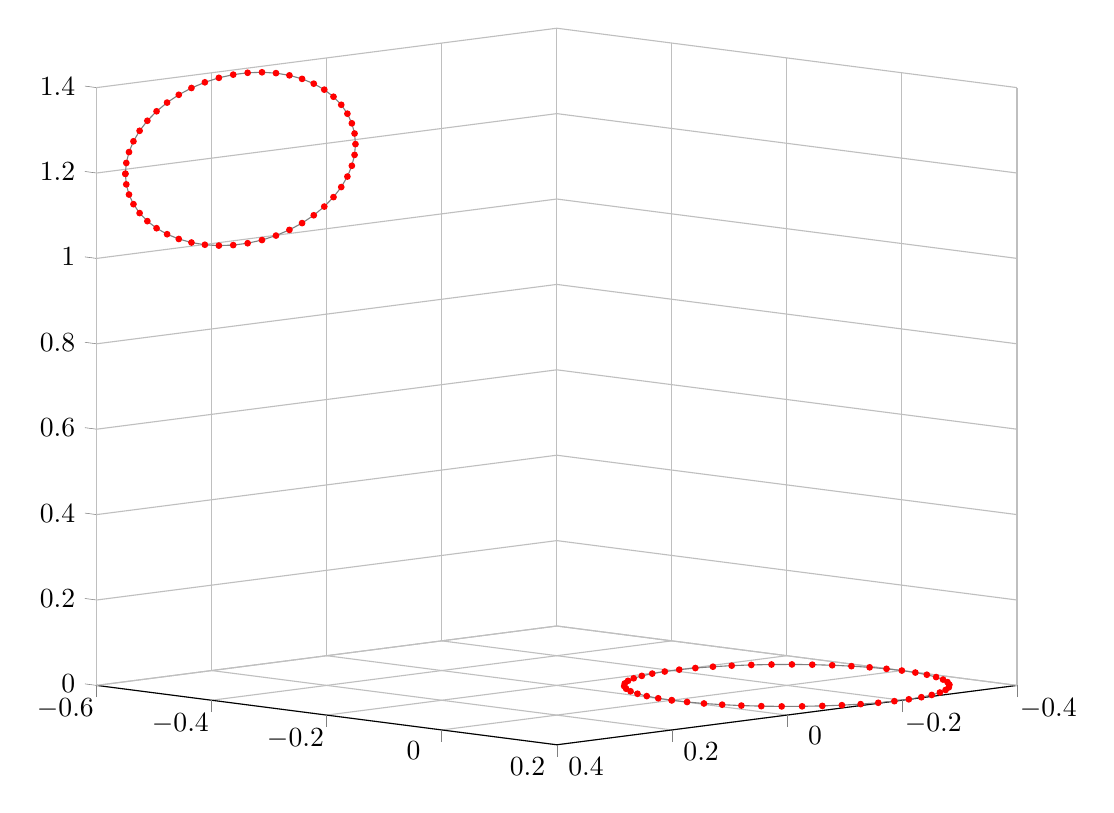
\begin{tikzpicture}

\begin{axis}[%
width=4.602in,
height=3.583in,
at={(0.772in,0.484in)},
scale only axis,
xmin=-0.4,
xmax=0.4,
tick align=outside,
ymin=-0.6,
ymax=0.2,
zmin=0,
zmax=1.4,
view={135}{8},
axis background/.style={fill=white},
%title style={font=\bfseries},
%title={Task priority dual trajectory},
axis x line*=bottom,
axis y line*=left,
axis z line*=left,
xmajorgrids,
ymajorgrids,
zmajorgrids
]
\addplot3 [color=red, draw=none, mark size=1pt, mark=*, mark options={solid, red}]
 table[row sep=crcr] {%
0.000163213509107997	-7.89364955824969e-06	0\\
-0.00141430163671715	0.0250591253559098	0\\
-0.00612089984096784	0.0497309181303326	0\\
-0.0138820472294895	0.073617381605015	0\\
-0.0245766043065936	0.0963445250638259	0\\
-0.0380338466782906	0.117549388773814	0\\
-0.0540438888928045	0.136902620283361	0\\
-0.0723531253970689	0.154096560082622	0\\
-0.0926716206171838	0.168857596054381	0\\
-0.114681550613838	0.180958381195553	0\\
-0.138034493768026	0.190205332969645	0\\
-0.16236100418229	0.1964503682861	0\\
-0.187278720427994	0.199597727900081	0\\
-0.212394988759989	0.199598627990254	0\\
-0.237312582900263	0.196453295669225	0\\
-0.261644163466932	0.190217126260767	0\\
-0.284998883902025	0.180972133480481	0\\
-0.307009025489303	0.168872816593898	0\\
-0.327328460052206	0.154109356940282	0\\
-0.345637149472391	0.13691532262126	0\\
-0.361647521885501	0.117564493187309	0\\
-0.375105156988281	0.0963573416836549	0\\
-0.38580006306724	0.0736335601602206	0\\
-0.393561475508085	0.0497465816613219	0\\
-0.398267197900361	0.0250737170595804	0\\
-0.399845349867462	9.0428717035848e-06	0\\
-0.398268060599071	-0.0250584254059232	0\\
-0.393562686763152	-0.0497283626795179	0\\
-0.385801744994137	-0.073615021740257	0\\
-0.375108285723675	-0.0963404748833795	0\\
-0.361651720056742	-0.117545134659854	0\\
-0.345643472635494	-0.136895996644418	0\\
-0.327335659585	-0.154088348933357	0\\
-0.307018172315592	-0.168849348642083	0\\
-0.285011289969987	-0.180946477096871	0\\
-0.261661298098012	-0.190189925758362	0\\
-0.237336132476052	-0.196434165753729	0\\
-0.212419519759077	-0.199580470572869	0\\
-0.187303089600662	-0.199580739561538	0\\
-0.162345640703185	-0.196480651963879	0\\
-0.138020395981644	-0.190232695780811	0\\
-0.114670499060875	-0.180984236756572	0\\
-0.0926633884269367	-0.168882020254835	0\\
-0.0723458730046985	-0.154117198306188	0\\
-0.0540389732329949	-0.136921732125155	0\\
-0.0380298249629342	-0.117569227317451	0\\
-0.0245729913732747	-0.0963617217624944	0\\
-0.0138800732611017	-0.073634606019589	0\\
-0.00611955983407252	-0.0497465959566359	0\\
-0.00141341020627131	-0.0250753402700977	0\\
0.000162729995430021	-7.19709673684629e-06	0\\
};
 \addplot3 [color=gray]
 table[row sep=crcr] {%
0.000159142246654337	5.27062717694817e-09	0\\
-0.00141791749045009	0.025066651983488	0\\
-0.00612422552761946	0.0497379827035981	0\\
-0.0138855605756954	0.0736249158075628	0\\
-0.024579521744573	0.0963507400909702	0\\
-0.0380374588783562	0.117557055729122	0\\
-0.0540471322690634	0.136909426456365	0\\
-0.0723560598036077	0.154102653825785	0\\
-0.0926754987575464	0.16886559037103	0\\
-0.114684999440331	0.180965415763831	0\\
-0.138037458878356	0.190211308529658	0\\
-0.162364594836201	0.196457455416365	0\\
-0.187282753847483	0.199605350956282	0\\
-0.212398961659208	0.199605350956282	0\\
-0.237317120670491	0.196457455416365	0\\
-0.261644256628335	0.190211308529658	0\\
-0.28499671606636	0.180965415763831	0\\
-0.307006216749145	0.16886559037103	0\\
-0.327325655703084	0.154102653825785	0\\
-0.345634583237628	0.136909426456365	0\\
-0.361644256628335	0.117557055729122	0\\
-0.375102193762118	0.0963507400909703	0\\
-0.385796154930996	0.0736249158075628	0\\
-0.393557489979072	0.0497379827035981	0\\
-0.398263798016241	0.0250666519834881	0\\
-0.399840857753346	5.27062720144111e-09	0\\
-0.398263798016241	-0.0250666414422337	0\\
-0.393557489979072	-0.0497379721623438	0\\
-0.385796154930996	-0.0736249052663085	0\\
-0.375102193762118	-0.0963507295497158	0\\
-0.361644256628335	-0.117557045187867	0\\
-0.345634583237628	-0.136909415915111	0\\
-0.327325655703084	-0.154102643284531	0\\
-0.307006216749145	-0.168865579829776	0\\
-0.28499671606636	-0.180965405222577	0\\
-0.261644256628335	-0.190211297988404	0\\
-0.237317120670491	-0.196457444875111	0\\
-0.212398961659208	-0.199605340415027	0\\
-0.187282753847483	-0.199605340415027	0\\
-0.162364594836201	-0.196457444875111	0\\
-0.138037458878356	-0.190211297988404	0\\
-0.114684999440331	-0.180965405222577	0\\
-0.0926754987575465	-0.168865579829776	0\\
-0.0723560598036078	-0.154102643284531	0\\
-0.0540471322690634	-0.136909415915111	0\\
-0.0380374588783562	-0.117557045187868	0\\
-0.024579521744573	-0.0963507295497159	0\\
-0.0138855605756954	-0.0736249052663086	0\\
-0.00612422552761946	-0.0497379721623439	0\\
-0.00141791749045012	-0.0250666414422338	0\\
0.000159142246654337	5.2706271279623e-09	0\\
};
 \addplot3 [color=gray]
 table[row sep=crcr] {%
0.356441821351327	-0.593546904582346	1.1917332419049\\
0.354864761614223	-0.593546904582346	1.21679988861776\\
0.350158453577053	-0.593546904582346	1.24147121933787\\
0.342397118528978	-0.593546904582346	1.26535815244184\\
0.3317031573601	-0.593546904582346	1.28808397672525\\
0.318245220226317	-0.593546904582346	1.3092902923634\\
0.30223554683561	-0.593546904582346	1.32864266309064\\
0.283926619301065	-0.593546904582346	1.34583589046006\\
0.263607180347127	-0.593546904582346	1.36059882700531\\
0.241597679664342	-0.593546904582346	1.37269865239811\\
0.218245220226317	-0.593546904582346	1.38194454516393\\
0.193918084268472	-0.593546904582346	1.38819069205064\\
0.16899992525719	-0.593546904582346	1.39133858759056\\
0.143883717445465	-0.593546904582346	1.39133858759056\\
0.118965558434182	-0.593546904582346	1.38819069205064\\
0.0946384224763378	-0.593546904582346	1.38194454516393\\
0.0712859630383127	-0.593546904582346	1.37269865239811\\
0.0492764623555279	-0.593546904582346	1.36059882700531\\
0.0289570234015893	-0.593546904582346	1.34583589046006\\
0.010648095867045	-0.593546904582346	1.32864266309064\\
-0.0053615775236622	-0.593546904582346	1.3092902923634\\
-0.0188195146574454	-0.593546904582346	1.28808397672525\\
-0.029513475826323	-0.593546904582346	1.26535815244184\\
-0.0372748108743989	-0.593546904582346	1.24147121933787\\
-0.0419811189115683	-0.593546904582346	1.21679988861776\\
-0.0435581786486727	-0.593546904582346	1.1917332419049\\
-0.0419811189115683	-0.593546904582346	1.16666659519204\\
-0.0372748108743989	-0.593546904582346	1.14199526447193\\
-0.029513475826323	-0.593546904582346	1.11810833136797\\
-0.0188195146574455	-0.593546904582346	1.09538250708456\\
-0.00536157752366223	-0.593546904582346	1.07417619144641\\
0.010648095867045	-0.593546904582346	1.05482382071917\\
0.0289570234015894	-0.593546904582346	1.03763059334975\\
0.049276462355528	-0.593546904582346	1.0228676568045\\
0.0712859630383128	-0.593546904582346	1.0107678314117\\
0.0946384224763378	-0.593546904582346	1.00152193864587\\
0.118965558434182	-0.593546904582346	0.995275791759166\\
0.143883717445465	-0.593546904582346	0.992127896219249\\
0.16899992525719	-0.593546904582346	0.992127896219249\\
0.193918084268472	-0.593546904582346	0.995275791759166\\
0.218245220226317	-0.593546904582346	1.00152193864587\\
0.241597679664342	-0.593546904582346	1.0107678314117\\
0.263607180347126	-0.593546904582346	1.0228676568045\\
0.283926619301065	-0.593546904582346	1.03763059334975\\
0.302235546835609	-0.593546904582346	1.05482382071917\\
0.318245220226317	-0.593546904582346	1.07417619144641\\
0.3317031573601	-0.593546904582346	1.09538250708456\\
0.342397118528978	-0.593546904582346	1.11810833136797\\
0.350158453577053	-0.593546904582346	1.14199526447193\\
0.354864761614223	-0.593546904582346	1.16666659519204\\
0.356441821351327	-0.593546904582346	1.1917332419049\\
};
 \addplot3 [color=red, draw=none, mark size=1pt, mark=*, mark options={solid, red}]
 table[row sep=crcr] {%
0.356441929185326	-0.593546990875446	1.19173577156017\\
0.3548648742698	-0.59354701347743	1.21680221551344\\
0.350158563552343	-0.593547034205783	1.24147330495562\\
0.342397238670973	-0.593547070733509	1.26536026686243\\
0.331703257157446	-0.593547062992473	1.28808562674396\\
0.318245343714857	-0.593547122952637	1.30929221466325\\
0.30223565572239	-0.593547115792351	1.32864427307269\\
0.283926715809694	-0.593547106293137	1.34583725272003\\
0.263607305526987	-0.593547182047314	1.36060052025012\\
0.241597788277453	-0.593547157175194	1.37270007404244\\
0.218245311148103	-0.593547124165707	1.38194570683725\\
0.193918190054799	-0.593547168761079	1.38819202595029\\
0.16900003550172	-0.593547190871473	1.39133998680885\\
0.143883807173566	-0.593547157928393	1.39133979058308\\
0.118965577728566	-0.593547066191176	1.38819134565241\\
0.0946382818880855	-0.593546700606857	1.38194330384538\\
0.0712858387067483	-0.593546667311663	1.3726972308647\\
0.0492763359475016	-0.593546656674274	1.36059724866681\\
0.0289569088790194	-0.593546684890823	1.34583435886088\\
0.0106479965311811	-0.593546723220304	1.3286412458062\\
-0.00536170239098635	-0.593546694708345	1.30928840500148\\
-0.0188196236467813	-0.593546737700587	1.28808221037025\\
-0.0295136164673827	-0.59354671543403	1.2653557141781\\
-0.0372749462058132	-0.593546747692022	1.24146867440369\\
-0.0419812245232457	-0.593546802253534	1.21679770504076\\
-0.0435583061352577	-0.593546809076511	1.19173032989784\\
-0.0419812259718515	-0.593546849255928	1.16666384605265\\
-0.0372749249975354	-0.593546876059159	1.14199193168947\\
-0.0295135804759175	-0.593546910361264	1.11810478769483\\
-0.0188196084940284	-0.59354694367357	1.09537871662216\\
-0.00536166750678505	-0.593546983334811	1.07417166571948\\
0.0106480176261884	-0.59354702423185	1.05481859422536\\
0.0289569655659369	-0.593547057282291	1.03762490486572\\
0.0492764247392141	-0.593547097720481	1.0228610810551\\
0.0712859478929328	-0.593547143073932	1.01076005744429\\
0.0946384300960315	-0.59354717987656	1.00151307902725\\
0.118965583581184	-0.593547204961167	0.99526609012255\\
0.143883752426866	-0.593547224196566	0.992117507865377\\
0.168999959859814	-0.593547220738819	0.992117620232243\\
0.193918059247512	-0.593546605252994	0.99528546214309\\
0.218245212612265	-0.593546629035454	1.00153080789835\\
0.241597694725674	-0.593546667345339	1.01077556503431\\
0.263607218434157	-0.593546708967866	1.0228743168652\\
0.283926678176569	-0.593546749099083	1.03763638524326\\
0.302235618632608	-0.593546794763884	1.05482861736882\\
0.318245312249189	-0.593546824026792	1.07418082017655\\
0.331703257934519	-0.593546862672681	1.09538657001411\\
0.342397221222551	-0.593546898913693	1.11811180935423\\
0.350158555939039	-0.59354693021456	1.14199825513624\\
0.354864875108535	-0.593546963024286	1.16666950637727\\
0.356441922751624	-0.593546980832727	1.19173556175769\\
};
 \end{axis}
\end{tikzpicture}%
%\end{figure}



\chapter{Conclusion}
Conclusion.

\bibliography{literatura}
\bibliographystyle{plainnat}

\appendix
\chapter{DH parameters}
\begin{table}
\caption{Thing's DH parameters}
 \begin{tabular}{@{}ccccc@{}}
  \toprule
 \textbf{Link}& $d_i$& $\theta_i$& $a_i$ & $\alpha_i$\\ \midrule \midrule
 \textbf{1} & $0$ & $\frac{\pi}{2}$ & $0$& $\frac{\pi}{2}$\\ \midrule
 \textbf{2} & $q_x$ & $\frac{\pi}{2}$ & $0$& $\frac{\pi}{2}$\\ \midrule
 \textbf{3} & $q_y$ & $\frac{\pi}{2}$ & $0$& $\frac{\pi}{2}$\\ \midrule
 \textbf{4} & $0$ &$q_{\theta}$ & 0& 0\\ \midrule
 \textbf{5} & $0.653$ & $0$ & 0.27& 0\\ \midrule
 \textbf{6} & $0$ & $\frac{\pi}{2}$ & 0.01& 0\\ \midrule
 \textbf{7} & $0.1273$ & $q_0$ & 0& $\frac{\pi}{2}$\\ \midrule
 \textbf{8} & $0$ & $q_1$ & -0.612& 0\\ \midrule
 \textbf{9} & $0$ & $q_2$ & -0.5723& 0\\ \midrule
 \textbf{10} & $ 0.163941$ & $q_3$ & 0& $\frac{\pi}{2}$\\ \midrule
 \textbf{11} & $0.1157$ & $q_4$ & 0& $-\frac{\pi}{2}$\\ \midrule
 \textbf{12} & $0.0922$ & $q_5$ & 0& 0\\ \bottomrule
 \end{tabular}
\label{DH}
\end{table}

\chapter{Robot operating system}\label{sec:def_ROS}
ROS is an open source software development tool for implementing robotics software. It provides the opportunity of hardware abstraction, low level device control, implementation of commonly used functionalities, messages between different processes and package management. It provide tools and libraries which utilize the the opportunity of communicating between disturbed computers, obtaining, writing and running code.


ROS has three different levels of concepts

\begin{itemize}
\item \textbf{The file system level}

Handles the main unit for a ROS system which is packages. A package may include data sets, ROS dependent libraries, configure files etc. to define a ROS process. In ROS a process is denoted as a node. 
\item \textbf{The computation graph level}

Handles the communication of the peer to peer network of the system in which data is processed. Through the computation graph level, the different nodes can communicate with each other by messages. When a node is sending data it is said to be publishing a topic. The different nodes can then subscribe to this topic to get the information that is published.
\item \textbf{The Community level}

ROS has a huge community which contain distribution of software installations, repositories and documentation of ROS. It also has a question and answer section with ROS related topics.\\
This community makes the process of learning the system considerably easier.
\end{itemize}
\begin{abstract}
Abstract.

\keywords{Keywords.}
\end{abstract}

% TODO: Navedite naslov na hrvatskom jeziku.
\hrtitle{Naslov}
\begin{sazetak}
Sažetak na hrvatskom jeziku.

\kljucnerijeci{Ključne riječi, odvojene zarezima.}
\end{sazetak}

\end{document}
